\documentclass[a4paper, 11pt, oneside, polutonikogreek, german]{article}
\usepackage{gfsbaskerville}
% Load encoding definitions (after font package)
\usepackage[LGR,T1]{fontenc}
\usepackage{wasysym}
\usepackage{textalpha}
\usepackage{longtable}

\usepackage{graphicx}
\graphicspath{ {./} }
\usepackage[figurename=]{caption}

\usepackage{listings}
\lstset{basicstyle=\ttfamily}
% Babel package:
\usepackage{babel}
\usepackage{yfonts}
% With XeTeX$\$LuaTeX, load fontspec after babel to use Unicode
% fonts for Latin script and LGR for Greek:
\ifdefined\luatexversion \usepackage{fontspec}\fi
\ifdefined\XeTeXrevision \usepackage{fontspec}\fi

% "Lipsiakos" italic font `cbleipzig`:
\newcommand*{\lishape}{\fontencoding{LGR}\fontfamily{cmr}%
		       \fontshape{li}\selectfont}
\DeclareTextFontCommand{\textli}{\lishape}

\usepackage{amssymb}
\usepackage{booktabs}
\setlength{\emergencystretch}{15pt}
\usepackage{fancyhdr}
\usepackage{microtype}
\usepackage[titles]{tocloft}
\usepackage{sectsty}

\allsectionsfont{\swabfamily }
\sectionfont{\swabfamily \LARGE}
\subsectionfont{\swabfamily \Large}
\subsubsectionfont{\swabfamily \large}

\paragraphfont{\large}

\usepackage[dvipsnames]{xcolor}
\usepackage{eso-pic,graphicx}
\usepackage[top=50mm, bottom=54mm, outer=47mm, inner=47mm]{geometry}
\setlength{\columnsep}{90pt}

\definecolor{customColor}{RGB}{218, 231, 228}

% change color of text, example replace all \color{Goldenrod} with \color{lightgray}

\makeatletter % change only the display of \thepage, but not \thepage itself:
\patchcmd{\ps@plain}{\thepage}{\swabfamily\color{customColor}{\thepage}}{}{}
\makeatother

\color{customColor}

\usepackage{setspace}
\onehalfspacing
\begin{document}
\swabfamily 
\renewcommand{\contentsname}{
\swabfamily {Inhaltsverzeichnis}
}

\renewcommand{\cftsecfont}{\swabfamily }
\renewcommand{\cftsubsecfont}{\swabfamily }
\renewcommand{\cftsubsubsecfont}{\swabfamily }

% fix toc page numbers
\let\origcftsecfont\cft
\let\origcftsecpagefont\cftsecpagefont
\let\origcftsecafterpnum\cftsecafterpnum
\renewcommand{\cftsecpagefont}{\swabfamily {\origcftsecpagefont}}
\renewcommand{\cftsecafterpnum}{\swabfamily {\origcftsecafterpnum}}
\let\origcftsubsecpagefont\cftsubsecpagefont
\let\origcftsubsecafterpnum\cftsubsecafterpnum
\renewcommand{\cftsubsecpagefont}{\swabfamily {\origcftsubsecpagefont}}
\renewcommand{\cftsubsecafterpnum}{\swabfamily {\origcftsubsecafterpnum}}
\let\origcftsubsubsecpagefont\cftsubsubsecpagefont
\let\origcftsubsubsecafterpnum\cftsubsubsecafterpnum
\renewcommand{\cftsubsubsecpagefont}{\swabfamily {\origcftsubsubsecpagefont}}
\renewcommand{\cftsubsubsecafterpnum}{\swabfamily {\origcftsubsubsecafterpnum}}

\renewcommand\thefootnote{\swabfamily{\arabic{footnote}}}
\AddToShipoutPictureBG{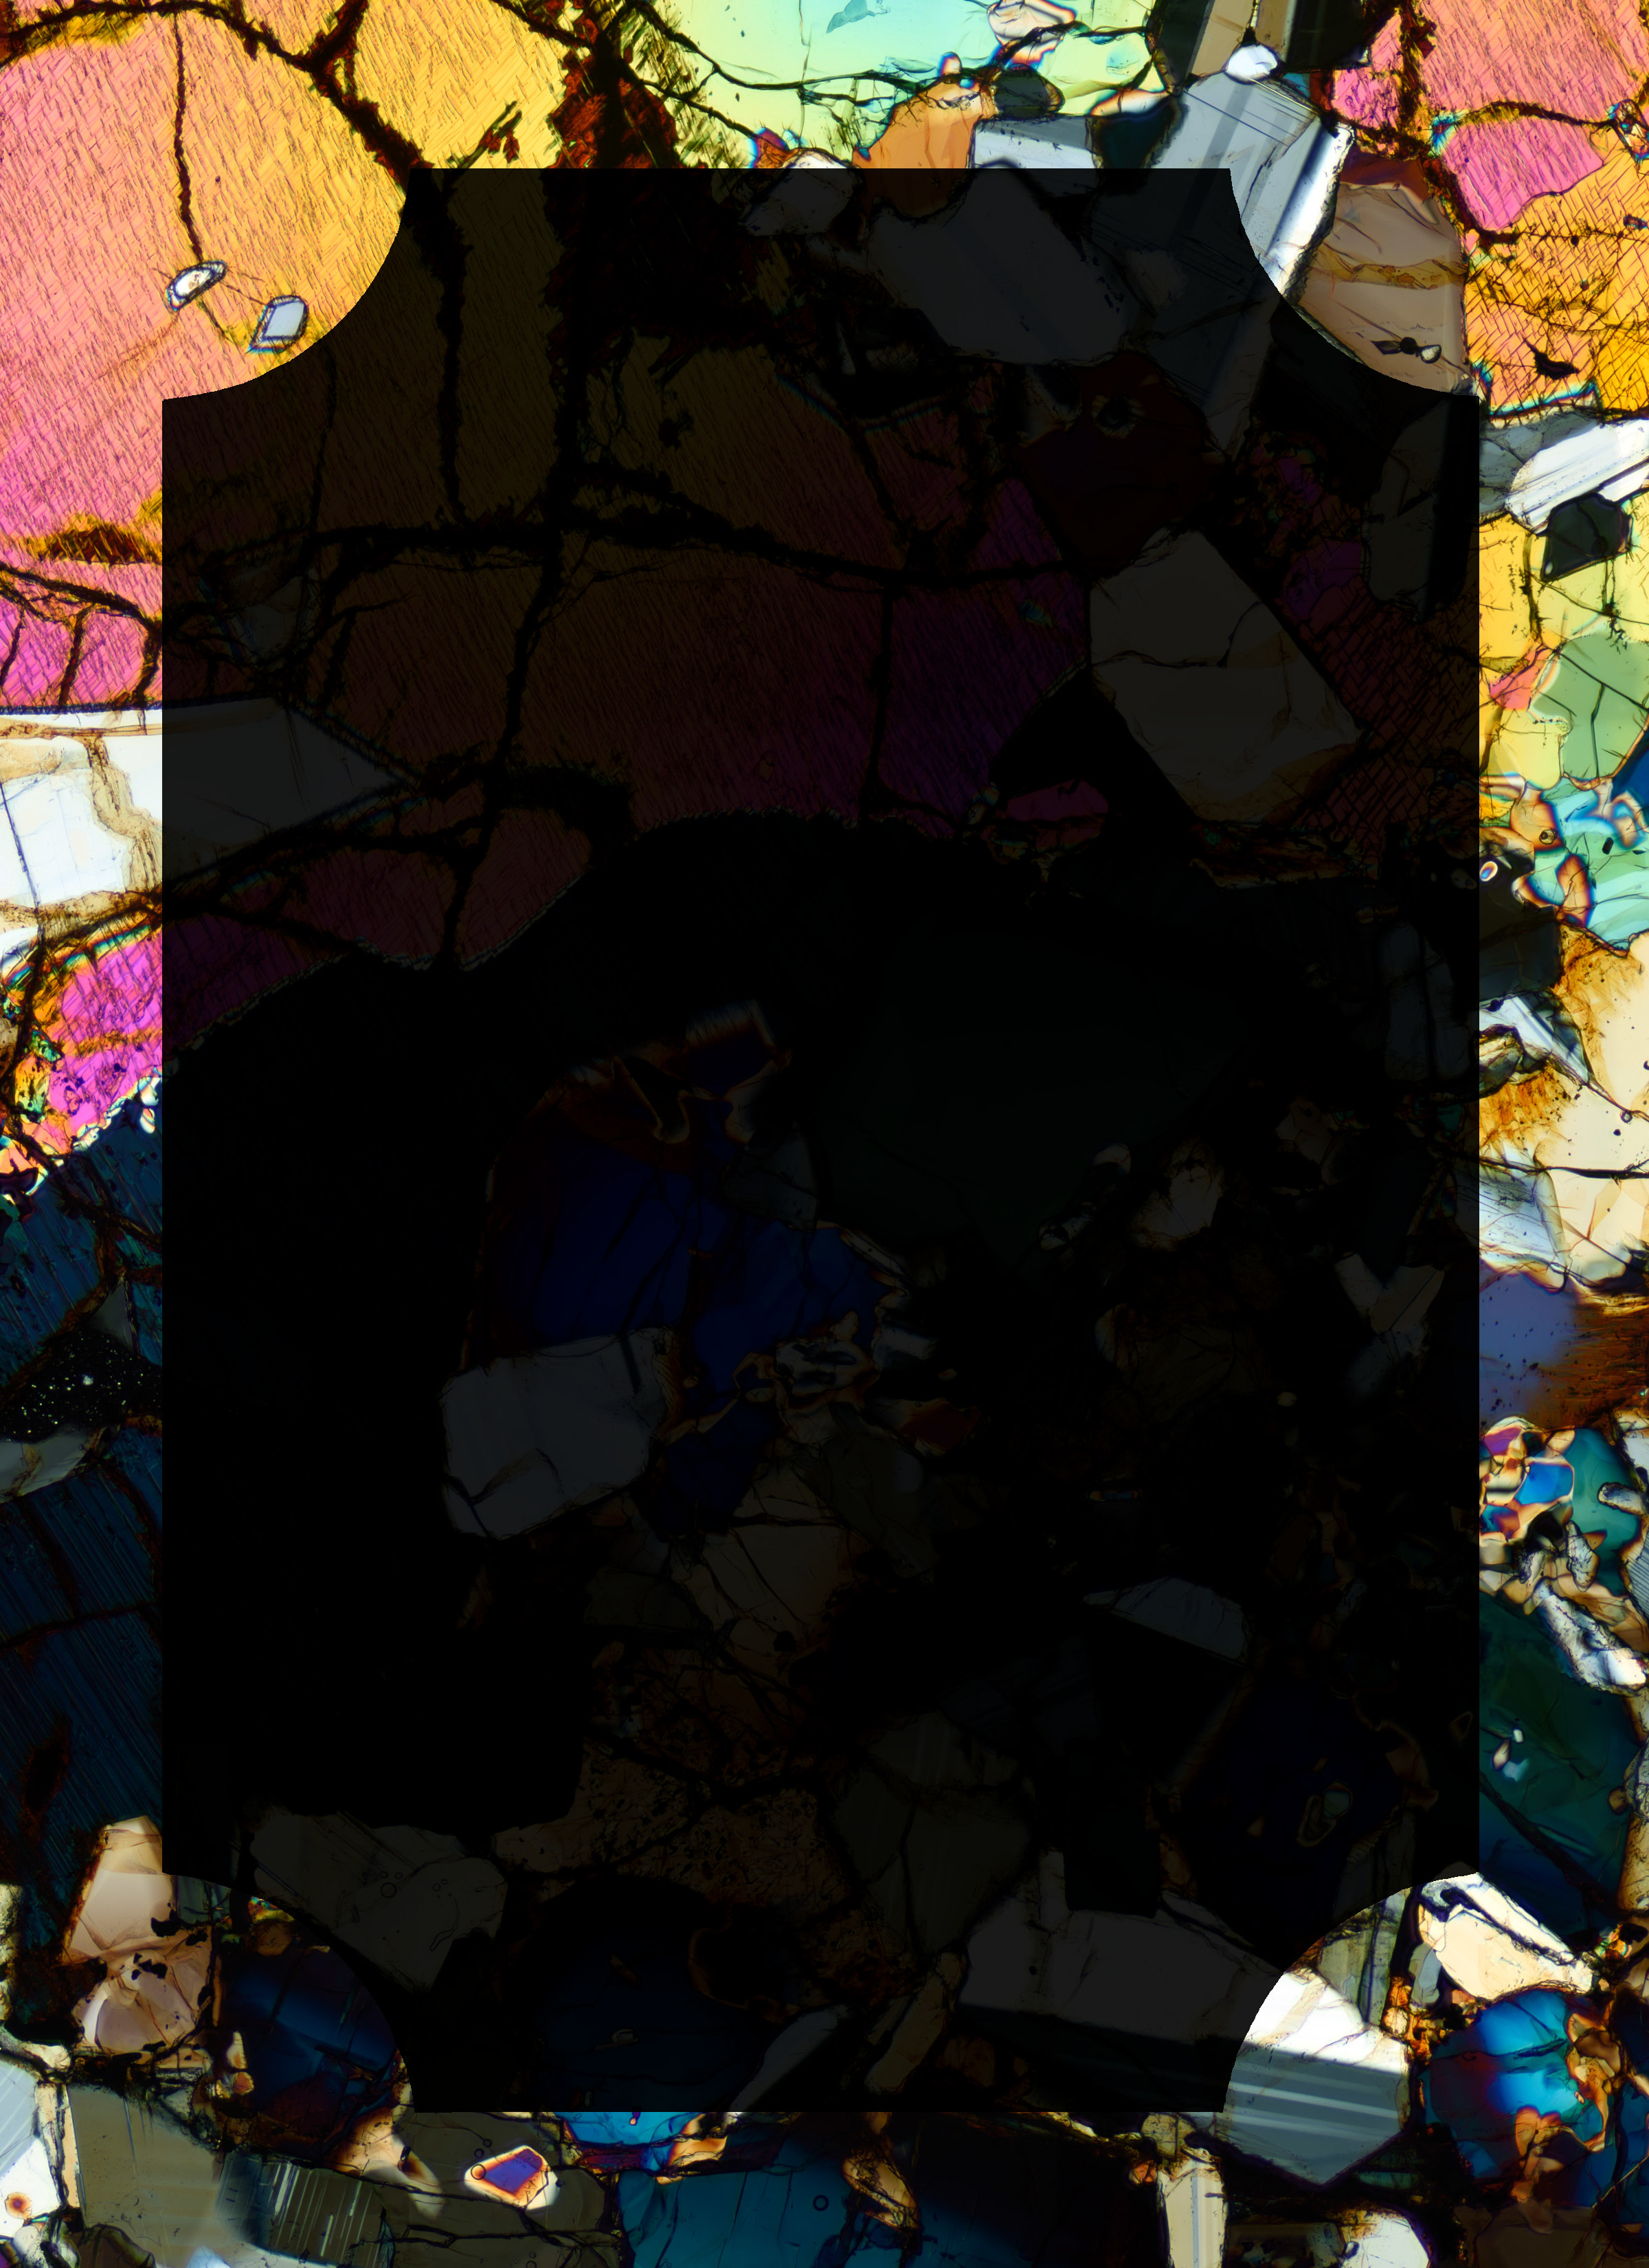
\includegraphics[width=\paperwidth,height=\paperheight]{angrite.jpeg}}
\begin{titlepage} % Suppresses headers and footers on the title page
	\centering % Centre everything on the title page
	%\scshape % Use small caps for all text on the title page

	%------------------------------------------------
	%	Title
	%------------------------------------------------
	
	\rule{\textwidth}{1.6pt}\vspace*{-\baselineskip}\vspace*{2pt} % Thick horizontal rule
	\rule{\textwidth}{0.4pt} % Thin horizontal rule
	
	\vspace{1\baselineskip} % Whitespace above the title
	
	{\scshape\Huge Die Meteoriten oder\\[1.25pt] vom Himmel gefallenen \\[1.25pt] Steine und Eisenmassen\\[1.25pt] im k. k. Hof-Mineralien-Kabinette\\[4pt] zu Wien.}
	
	\vspace{1\baselineskip} % Whitespace above the title

	\rule{\textwidth}{0.4pt}\vspace*{-\baselineskip}\vspace{3.2pt} % Thin horizontal rule
	\rule{\textwidth}{1.6pt} % Thick horizontal rule
	
	\vspace{1\baselineskip} % Whitespace after the title block
	
	%------------------------------------------------
	%	Subtitle
	%------------------------------------------------
	
	{\Large Beschrieben,\\ und durch wissenschaftliche und geschichtliche \\ Zus"atze erl"autert \\ von \\ Paul Partsch,} % Subtitle or further description
	
	\vspace*{1\baselineskip} % Whitespace under the subtitle
	
        {Kustos an dem genannten Kabinette. \\ Mit einer Abbildung.} % Subtitle or further description
    
	%------------------------------------------------
	%	Editor(s)
	%------------------------------------------------
        \vspace*{\fill}

	\vspace{1\baselineskip}

	{\scshape Wien 1843.}
	
	{\scshape{Verlag von Kaulfuss Witwe, Prandel \& Komp.}}
	
	\vspace{0.5\baselineskip} % Whitespace after the title block

    \scshape Internet Archive Online Edition  % Publication year
	
	{\scshape Namensnennung Nicht-kommerziell Weitergabe unter gleichen Bedingungen 4.0 International} % Publisher
\end{titlepage}
\setlength{\parskip}{1mm plus1mm minus1mm}
\clearpage
\pagestyle{fancy}
\fancyhf{}
\cfoot{\swabfamily {\thepage}}
\tableofcontents
\clearpage
\Large
\vspace*{\fill}
\begin{quote}
   Es l"asst sich als ausgemacht ansehen, dass sie nicht von der Erde, sondern von einem anderen Weltk"orper herstammen, und folglich die Beschaffenheit der au"serhalb der Erde vorkommenden w"agbaren Stoffe verk"unden. In dieser Beziehung haben die Meteorsteine ein au"serordentliches Interesse. --- Berzelius
\end{quote}
\vspace*{\fill}
\clearpage
\section*{\swabfamily {Vorwort.}}
\paragraph{}
In dem k. k. Hof-Mineralien-Kabinette zu Wien befinden sich acht Sammlungen in Glasschr"anken zur Schau gestellt, die jede Woche zweimal, Mittwoche und Sonnabend, von Jedermann besehen und ben"utzt werden k"onnen. Nachdem der Herausgeber vorliegender Schrift eine kurze allgemeine "Ubersicht dieser Sammlungen des k. k. Mineralien-Kabinettes k"urzlich in Druck gelegt hat, beginnt er das darin gegebene Versprechen, von jeder derselben, je nach Bed"urfnis und Zweckm"a"sigkeit, entweder spezielle Verzeichnisse oder doch ausgedehntere "Ubersichten nachfolgen zu lassen, dadurch in Ausf"uhrung zu bringen, dass er zuerst das vorliegende beschreibende Verzeichnis erscheinen l"asst. Die Meteoriten-Sammlung des k. k. Mineralien-Kabinettes ist zwar von allen daselbst befindlichen der Anzahl der St"ucke nach die kleinste, aber doch die reichste und vollst"andigste in der Anzahl von Lokalit"aten und Exemplaren unter allen bestehenden Sammlungen ihrer Art, und "uberhaupt eine der merkw"urdigsten Zusammenstellungen von unorganischen K"orpern.\footnote{\swabfamily {Die Meteoriten-Sammlung des k. k. Mineralien-Kabinettes enthielt im Monate Februar 1843, mit Ausschluss aller Pseudometeoriten, die wir sp"ater anf"uhren werden, 94 verschiedene Lokalit"aten von Meteoriten, und zwar 69 von Meteorsteinen, und 25 von Meteoreisen in 258 St"ucken oder eigentlich Nummern, da zuweilen mehrere kleine St"ucke unter Einem Nummer vereinigt sind. (Im Jahre 1806 z"ahlte sie 7, im Jahre 1819. 36, im Jahre 1836. 58 Lokalit"aten.) --- Von Meteoriten, mit Ausschluss aller Pseudometeoriten, besa"sen zwischen den Jahren 1840 und 1842: das k. Mineralien-Kabinett der Universit"at zu Berlin, mit welcher die Sammlung Chladnis vereinigt ist, 78 Lokalit"aten; Baron Reichenbach in Wien 68 (wovon jedoch 19 nur in kleinen Splittern); die Galerie der Mineralogie im k. Museum der Naturgeschichte zu Paris 42; Gubernialrat Neumann in Prag 40 (meistens in ganz kleinen Fragmenten); die Mineralien-Sammlung im britischen Museum zu London und die Mineralien-Sammlung der Universit"at zu G"ottingen jede 35; Professor John in Berlin 28 (ebenfalls meist in ganz kleinen St"uckchen); die Mineralien-Sammlung der Akademie der Wissenschaften zu St. Petersburg und Baron Berzelius in Stockholm 18; Stra"senbaudirektor Braum"uller zu Br"unn 17; die Mineralien-Sammlung des Herrn Turner in England, ehemals Eigentum des H. Heuland in London 15; die Mineralien-Sammlung des Marquis de Drée zu Paris 14. Diess sind die an Meteoriten reichsten Sammlungen; andere "offentliche und Privat-Sammlungen besitzen selten mehr als 12 Lokalit"aten; so die Ecole des Mines zu Paris und die Mineralien-Sammlung des Grafen Beroldingen in Wien 12; die Privat-Mineralien-Sammlung des K"onigs von D"anemark zu Kopenhagen 11; das herzogliche Naturalien-Kabinett zu Gotha 10; die Mineralien-Sammlung der Universit"at zu Uppsala, die Mineralien-Sammlung der Akademie der Wissenschaften zu M"unchen, Professor Pfaff zu Kiel und die Universit"ats-Sammlung in Parma 9; das Joanneum zu Gr"atz und die Sammlungen der Bergakademie zu Freiberg 8; die Mineralien-Sammlung der Universit"at zu Wilna, jetzt in Kiew 7; die Mineralien-Sammlung der vaterl"andischen Museen zu Prag und Pesth, dann die der Prager Universit"at jede 6; u. s. w. Die Meteoriten-Sammlung, die von Herrn Heinrich Heuland in London zusammengebracht sp"ater Eigentum des Herrn Heath zu Madras in Ostindien wurde, z"ahlte 43 Lokalit"aten von echten Meteoriten. Nach Europa zur"uckgebracht, wurden sie im Jahre 1837 von Herrn Carl P"otschke in Wien angekauft und daselbst vereinzelt.}} Wer w"urde denn nicht mit ungew"ohnlichem Interesse eine so gro"se Anzahl jener r"atselhaften Ank"ommlinge von Au"sen hier vereiniget betrachten ? diese aus dem gro"sen Weltraume oberhalb unserer Atmosph"are stammenden Massen (entweder fest gewordene kosmische Materie, oder St"ucke eines zersprungenen Planeten), daher vom Himmel gefallene Steine und Eisenmassen genannt, Aerolithen oder Luftsteine von denjenigen, die ihre Entstehung in unserer Atmosph"are suchen, Mondsteine von denen, die sie durch Vulkane oder elektrische Entladungen aus diesem Erdtrabanten ausschleudern lassen, gew"ohnlich aber Meteorsteine und Meteoreisen, oder mit einem gemeinschaftlichen Nahmen Meteoriten genannt, weil sie am Himmel als Meteore oder Feuerkugeln erscheinen, aus welchen, unter heftigem Schall und Geprassel, jene Massen, meist Steine, seltener wunderbare Eisenbl"ocke, noch hei"s und nach Schwefel riechend, auf die Erde niederst"urzen. Das schon seit den "altesten Zeiten beobachtete Niederfallen dieser Massen auf unseren Planeten hat von jeher den gr"o"sten Eindruck auf das menschliche Gem"ut gemacht, daher mehrere V"olker des Altertums, Ph"onizier, Griechen, R"omer u. a. m., die sie heilige Steine oder B"atylien nannten, ihnen, zumal als Symbol der Mutter der G"otter, abergl"aubische Verehrung bezeigten, und dieselben, wie uns alte Geschichtsschreiber und antike M"unzen lehren, in Tempeln aufbewahrten und in Triumphz"ugen herumf"uhrten.\footnote{\swabfamily {M"unter: "Uber die vom Himmel gefallenen Steine, B"atylien genannt, Kopenhagen und Leipzig 1805. 8, (auch in Gilberts Annalen der Physik, B. 21, S. 51-84, unter dem Titel: Vergleichung der B"atylien der Alten mit den Steinen, welche in neueren Zeiten vom Himmel gefallen sind.) --- Von Dalberg: "Uber Meteor-Cultus der Alten, vorz"uglich in Bezug auf Steine, die vom Himmel gefallen. Heidelberg 1811. 8.}} Obwohl das Ereignis des Niederfallens durch mehrere Dezennien des vorigen Jahrhunderts bezweifelt, ja hartn"ackig geleugnet, die daran Glaubenden verspoltet und verlacht wurden, so hat dieser Gegenstand seit dem ber"uhmten Steinregen von L’Aigle in der Normandie am 26. April 1803, den das franz"osische National-Institut durch sein Mitglied, den bekannten Physiker, Herrn Biot, untersuchen lie"s, in neuerer Zeit doch so viel allgemeine Aufmerksamkeit erregt, und so verschiedene Untersuchungen und Beleuchtungen von Seite der Gelehrten zur Folge gehabt, dass jeder Gebildete, namentlich seit dem Erscheinen der verdienstvollen Schriften von Izarn\footnote{\swabfamily {Des pierres tombées du ciel ou Lithologie atmosphérique. Paris 1803. 8.}} und Bigot de Morogues,\footnote{\swabfamily {Mémoire historique et physique sur les chutes des pierres tombées sur la surface de la terre a diverses époques. Orléans 1812. 8.}} vorz"uglich aber durch die klassischen Arbeiten von Howard,\footnote{\swabfamily {Experiments and Observations on certain stony and metalline Substances, wich at different Times are said to have fallen on the Earth, also on various Kinds of native Iron, in den Philos. Transact. of the Roy. Soc. of London for 1802. Part 1. S. 168; deutsch in Gilberts Annalen der Physik, B. 13, S. 291, unter dem Titel: Versuche und Bemerkungen "uber Stein- und Metallmassen, die zu verschiedenen Zeiten auf die Erde gefallen sein sollen, und "uber die gediegenen Eisenmassen.}} Chladni\footnote{\swabfamily {"Uber Feuer-Meteore und "uber die mit denselben herabgefallenen Massen. Wien 1819, im Verlage bei J. G. Heubner. 8. Nebst vielen Aufs"atzen in Gilberts Annalen.}} und Karl von Schreibers\footnote{\swabfamily {Nachrichten von dem Steinregen zu Stannern in M"ahren, in Gilberts Annalen der Physik. B. 29. 1808. S. 225. --- Beitr"age zur Geschichte und Kenntnis meteorischer Stein- und Metallmassen und der Erscheinungen, welche deren Niederfallen zu begleiten pflegen, Wien 1820, im Verlage von J. G. Heubner, Folio. Mit Abbildungen. --- "Uber den Meteorstein-Niederfall auf der Herrschaft Wessely in M"ahren, in Baumgartners Zeitschrift f"ur Physik und verwandte Wissenschaften. B. 1. 1832. S. 193-256.}} wenigstens mit den Tatsachen des Ph"anomens, wenn auch nicht "uber die Herkunft dieser merkw"urdigen Massen, die uns nie v"ollig klar werden, und immer Gegenstand mehr oder weniger gewagter Theorien bleiben wird, im Reinen ist. Die erw"ahnten wissenschaftlichen Untersuchungen haben jedoch in der naturhistorischen Betrachtung der Meteorsteine und Meteoreisenmassen, zu denen die Arbeiten des Herrn von Schreibers, des verdienstvollen Gr"unders unserer Meteoriten-Sammlung, und die technischen Untersuchungen einiger Meteoreisenmassen durch Herrn von Widmannst"atten den Grund legten, ungeachtet der sch"onen Beitr"age, welche die Herren Gustav Rose\footnote{\swabfamily {Poggendorffs Annalen der Physik und Chemie. B. 4. S. 173.}} und Cordier,\footnote{\swabfamily {Annales de Chemie et de Physique. T. 34. pag. 132.}} vorz"uglich aber Berzelius\footnote{\swabfamily {Poggendorffs Annalen. Bd. 33. S. 1 und 113 auch Jahresbericht "uber die Fortschritte der physischen Wissenschaften 15. Jahrgang S. 227.}} dazu in neuerer Zeit lieferten, noch gro"se L"ucken in der genauen naturhistorischen Kenntnis dieser r"atselhaften K"orper gelassen. Die Ursache mag darin liegen, dass nur wenige bedeutende Sammlungen von Meteoriten bestehen, und in diesen wenigen diese kostbaren Produkte nicht in jenem Zustande vorhanden sind, der zu einer genauen Untersuchung und Kenntnis dieser, gleich den Gebirgsarten gemengten Massen unumg"anglich notwendig ist; n"amlich in einem durch k"unstliche Zubereitung entstehenden Zustand, der ihr Inneres aufschlie"st, und ihre wahre Beschaffenheit erst kennen lehrt. Wir meinen die Anfertigung von gut polierten Schnittfl"achen bei Meteorsteinen; von fein polierten Schnittfl"achen, die sonst keine andere Ver"anderung zu erleiden brauchen, dann von polierten Fl"achen, die weiter entweder durch Hitze-Einwirkung blau, violett oder rot anlaufen gemacht, oder durch Anwendung von metallischen S"auren (Salz- oder Salpeters"aure) mehr oder weniger stark ge"atzt worden sind, bei Meteoreisenmassen. Da dieses mit vieler M"uhe und gro"sem Zeitaufwande, mit nicht unbedeutenden Kosten und nicht geringer Verminderung des Volums und Gewichts der so wertvollen Meteoriten in der Sammlung des k. k. Mineralien-Kabinettes ausgef"uhrt worden ist (die "Atzung der Eisenmassen meist von Herrn von Widmannst"atten, dem Entdecker der nach ihm benannten merkw"urdigen Figuren), so bietet sie ganz allein unter allen bestehenden Meteoriten-Sammlungen Gelegenheit dar, die Eigenschaften, den Charakter und die Verwandtschaften der Meteoriten vollst"andig ins Klare zu bringen. Dieser Umstand hat uns bestimmt, dieselben nach den einzelnen Lokalit"aten mit kurzen Beschreibungen oder Diagnosen zu versehen, durch die Darstellung ihrer Anordnung und ihrer Reihenfolge und eine angeh"angte Verwandtschaftstabelle die "Ahnlichkeiten und Verschiedenheiten, die sie darbieten (wovon die ersteren im Allgemeinen geringer, die anderen viel gr"osser sind, als sich mancher Mineraloge vorstellt), zu zeigen, ohne dabei jedoch in eine mikroskopische Untersuchung der Meteorsteine einzugehen, die besseren Augen vorbehalten bleibt und wozu einer der ausgezeichnetsten hiesigen Gelehrten, selbst im Besitze einer der bedeutendsten Meteoriten-Sammlungen und, was bei derlei Untersuchungen fast unumg"anglich notwendig ist, zugleich Chemiker, bereits zahlreiche Materialien gesammelt hat, deren baldige Bekanntmachung zu w"unschen ist. Wir haben somit, soweit es der Hauptzweck dieses beschreibenden Verzeichnisses gestattete (das "ubrigens mit Ausschluss der Tabellen, Anmerkungen, Zus"atze u. s. w. gr"o"stenteils ein Abdruck des von uns verfassten amtlichen Kabinetts-Kataloges ist) bei der Herausgabe desselben gestrebt, zugleich einen wissenschaftlichen Beitrag zur Kenntnis der Meteoriten zu geben, In dieser Absicht haben wir auch am Schlusse eine Tabelle "uber die spezifischen Gewichte s"amtlicher im k. k. Mineralien-Kabinette aufbewahrter Meteoriten beigef"ugt. Die Wiegungen hat der Kustos-Adjunkt an diesem Kabinette Herr Karl Rumler mit aller Sorgfalt bei einer Temperatur von 140 R. ausgef"uhrt, und es wurden dieser Tabelle auch alle anderen in verschiedenen Werken und Abhandlungen zerstreuten Angaben der spezifischen Gewichte von Meteoriten und auch einige noch nicht ver"offentlichte beigef"ugt. Die historischen Beigaben und erl"auternden wissenschaftlichen Anmerkungen werden Wissenschaftsfreunden in diesen Bl"attern vielleicht ebenfalls nicht unwillkommen sein. Noch manches Material (worunter sch"on ausgef"uhrte Zeichnungen von s"amtlichen durch "Atzen bei den verschiedenen Meteoreisenmassen zum Vorschein kommenden Figuren), liegt zur Bekanntmachung bereit, und wird, falls die Annalen des Wiener Museums der Naturgeschichte wieder aufleben sollten, dem Publikum vorgelegt werden. M"oge dasjenige, was wir hier bieten, ein freundliches Andenken denjenigen sein, die Gelegenheit haben, die Meteoriten-Sammlung des k. k. Mineralien-Kabinettes zu sehen und Anderen, namentlich Eigent"umern oder Vorstehern von Mineralien-Sammlungen, Besitzern von einzelnen Meteoriten u. s. w. Veranlassung werden, der Sammlung des k. k. Mineralien-Kabinettes im Interesse der Wissenschaft Bereicherungen an Meteoriten zukommen zu lassen. F"ur eine bereits so reiche Sammlung ist jede neue Lokalit"at ein hochanzuschlagender Gewinn, und daher dem Geber (nebst der Gegengabe von anderen Meteoriten oder Mineralien, wenn es gew"unscht wird), der vollste Dank gesichert.

Wien, den 23. Februar 1843.
\clearpage
\section{\swabfamily {"Ubersicht der Meteoriten im k. k. Mineralien-Kabinette nach der Reihenfolge ihrer Aufstellung.}}
\begin{center}
(Die Nummern dienen zur Erleichterung des Aufsuchens im vorliegenden Kataloge.)
\end{center}
\subsection{\swabfamily {Meteorsteine.}}
\begin{enumerate}
    \item Alais (St. Etienne de Lolm und Valence).
    \item Simonod
    \item Kapland (Bokkeveld).
    \item Chassigny (Langres).
    \item Juvenas.
    \item Stannern.
    \item Konstantinopel.
    \item Jonzac.
    \item Bialistock.
    \item Lontalax.
    \item Nobleborough (Nobleboro, Maine).
    \item M"assing (Eggenfelden).
    \item Parma (Casignano).
    \item Siena.
    \item Ensisheim.
    \item L'Aigle.
    \item Liponas.
    \item Chantonnay.
    \item Renazzo (Ferrara).
    \item Richmond (Virginien).
    \item Weston (Connecticut).
    \item La Baffe (Épinal).
    \item Benares (Krakhut).
    \item Gouv. Poltawa.
    \item Krasno-Ugol.
    \item Erxleben.
    \item Gouv. Simbirsk.
    \item Mauerkirchen.
    \item Nashville (Tennessee).
    \item Lucé.
    \item Lissa.
    \item Owahu (Hanaruru).
    \item Charkow (Ukraine).
    \item Zaborzika.
    \item Bachmut.
    \item Politz (K"ostriz).
    \item Kuleschofka.
    \item Slobodka.
    \item Milena.
    \item Forsyth (Georgien).
    \item Yorkshire (Wold-Cottage).
    \item Glasgow (High Possil).
    \item Berlanguillas (Burgos).
    \item Apt (Saurette).
    \item Vouillé (Poitiers).
    \item Château-Renard (Triguères).
    \item Salés (Villefranche).
    \item Agen.
    \item Nanjemoy (Maryland).
    \item Asco.
    \item Toulouse.
    \item Blansko.
    \item Wessely.
    \item Limerick (Adair).
    \item Gr"uneberg (Heinrichau).
    \item Tipperary (Mooresfort).
    \item Gouv. Kursk.
    \item Lixna (D"unaburg).
    \item Tabor (Plan).
    \item Charsonville (Orléans).
    \item Doroninsk.
    \item Seres (Makedonien).
    \item Sigena (Sena).
    \item Barbotan (Roquefort, Créon Juillac).
    \item Eichst"adt (Wittens).
    \item Gro"s-Divina (Budetin).
    \item Zebrak (Horzowitz).
    \item Timochin (Smolensk).
    \item Macao (Rio Assu).
\end{enumerate}
\subsection{\swabfamily {Meteoreisen.}}
\begin{enumerate}
    \item Atacama.
    \item Krasnojarsk (Sibirien, Pallas).
    \item Brahin.
    \item Sachsen (Steinbach oder Grimma ? mit dem Eisen, angeblich aus Norwegen).
    \item Bitburg.
    \item Toluca (Xiquipilco).
    \item Elbogen.
    \item Agram (Hraschina).
    \item Lenarto.
    \item Red-River (Louisiana oder Texas).
    \item Durango.
    \item Guilford.
    \item Caille (Grasse).
    \item Ashville (Buncombe).
    \item Tennessee.
    \item Bohumilitz.
    \item Bahia (Bemdegò).
    \item Zacatecas.
    \item Rasgatà.
    \item Tucuman (Otumpa).
    \item Senegal.
    \item Kap der guten Hoffnung.
    \item Clairborne (Alabama).
\end{enumerate}
\subsection{\swabfamily {Anhang.}}
\begin{enumerate}
    
    \item Oaxaca.
    \item Gr"onland (Baffingsbay).
\end{enumerate}
\clearpage
\section{\swabfamily {"Ubersicht der Meteoriten im k. k. Mineralien-Kabinette, nach den Fall- oder Fundorten.}}
\begin{center}

(Die Nummern beziehen sich auf die Reihenfolge in der "Ubersicht Nr. 1., und dienen zur Erleichterung des Aufsuchens im vorliegenden Kataloge.)
\end{center}
\subsection{\swabfamily {Meteorsteine.}}
\subsubsection{\swabfamily {Europa}}
\begin{center}
Frankreich.
\end{center}
\begin{itemize}
    
    \item[48.] Agen, Dépt. Lot et Garonne.
    \item[1.] Alais, Dépt. du Gard.
    \item[44.] Apt, Dépt. de Vaucluse.
    \item[50.] Asco, Insel Korsika.
    \item[64.] Barbotan (und Roquefort) ehemals Gascogne, Dépt. du Gers (und Dépt. des Landes).
    \item[18.] Chantonnay, Dépt. de la Vendée.
    \item[60.] Charsonville, Dépt. du Loiret.
    \item[4.] Chassigny, Dépt. de la haute Marne.
    \item[46.] Château-Renard, Dépt. du Loiret.
    \item[15.] Ensisheim, ehemals Elsass, jetzt Dépt. du Haut-Rhin.
    \item[8.] Jonzac, Dépt. de la Charente inferieure.
    \item[5.] Juvenas, Dépt. de l'Ardeche.
    \item[22.] La Baffe, Dépt. des Vosges.
    \item[16.] L'Aigle, ehemals Normandie, Dépt. de l'Orne.
    \item[17.] Liponas, Dépt. de l'Ain.
    \item[30.] Lucé, Dépt. de la Sarthe.
    \item[47.] Salés, Dépt. du Rhone.
    \item[2.] Simonod, Dépt. de l'Ain.
    \item[51] Toulouse, Dépt. de la Haute-Garonne.
    \item[45] Vouillé, Dépt. de la Vienne.
\end{itemize}
\begin{center}
England.
\end{center}
\begin{itemize}
    
    \item[41.] Wold-Cottage, Yorkshire.
\end{itemize}
\begin{center}
Schottland.
\end{center}
\begin{itemize}
    
    \item[42.] High-Possil, Glasgow.
\end{itemize}
\begin{center}
Irland.
\end{center}
\begin{itemize}
    
    \item[56.] Mooresfort, Grafschaft Tipperary.
    \item[54.] Adair, Grafschaft Limerick.
\end{itemize}
\begin{center}
Spanien.
\end{center}
\begin{itemize}
    
    \item[43.] Berlanguillas, Alt-Kastilien.
    \item[63.] Sigena, Aragonien.
\end{itemize}
\begin{center}
Italien.
\end{center}
\begin{itemize}
    
    \item[13.] Casignano, Herzogtum Parma.
    \item[19.] Renazzo, Provinz Ferrara, Kirchenstaat.
    \item[14.] Siena, Toskana.
\end{itemize}
\begin{center}
Deutschland.
\end{center}
\begin{itemize}
    
    \item[59.] Tabor, ehemals Bechiner, jetzt Taborer Kreis, B"ohmen.
    \item[67.] Zebrak, Berauner Kreis, B"ohmen.
    \item[31.] Lissa, Bunzlauer Kreis, B"ohmen.
    \item[6.] Stannern, Iglauer Kreis, M"ahren.
    \item[52.] Blansko, Br"unner Kreis, M"ahren.
    \item[53.] Wessely, Hradischer Kreis, M"ahren.
    \item[28.] Mauerkirchen, ehemals Bayern, jetzt Inn-Kreis, Ober-"Osterreich.
    \item[12.] M"assing, Unter-Donau-Kreis, Niederbaiern.
    \item[65.] Eichst"adt, Regenkreis, Franken, Baiern.
    \item[36.] Politz bei Gera, F"urstentum Reu"s.
    \item[26.] Erxleben, Regierungsbezirk Magdeburg, preu"sische Provinz Sachsen.
    \item[55.] Gr"uneberg, Regierungsbezirk Liegnitz, Provinz Schlesien.
\end{itemize}
\begin{center}
Ungarn.
\end{center}
\begin{itemize}
    
    \item[66.] Gro"s-Divina, Trentschiner-Komitat.
\end{itemize}
\begin{center}
Kroatien.
\end{center}
\begin{itemize}
    
    \item[39.] Milena, Warasdiner-Komitat.
\end{itemize}
\begin{center}
Russland.
\end{center}
\begin{itemize}
    
    \item[35.] Bachmut, Gouv. Ekaterinoslaw.
    \item[9.] Bialistock, gleichnamige Provinz.
    \item[33.] Charkow, gleichnamiges Gouvernement.
    \item[25.] Krasno-Ugol, Gouv. R"asan.
    \item[37.] Kuleschofka, Gouv. Poltawa.
    \item[57.] Kursk (Gouv.)
    \item[58.] Lixna, D"unaburger Kreis, Gouv. Witepsk.
    \item[10.] Lontalax, Finnland.
    \item[24.] Poltawa (Gouv.)
    \item[27.] Simbirsk (Gouv.)
    \item[38.] Slobodka, Gouv. Smolensk.
    \item[68.] Timochin, Gouv. Smolensk.
    \item[34.] Zaborzika, Gouv. Wolhynien.
\end{itemize}
\begin{center}
T"urkei.
\end{center}
\begin{itemize}
    
    \item[7.] Konstantinopel.
    \item[62.] Seres, Makedonien.
\end{itemize}
\subsubsection{\swabfamily {Asien.}}
\begin{itemize}
    
    \item[61.] Doroninsk, Gouv. Irkutsk, Sibirien.
    \item[23.] Benares, Bengalen, Ostindien.
\end{itemize}
\subsubsection{\swabfamily {Afrika.}}
\begin{itemize}
    
    \item[3.] Kapland (Bokkeveld bei Tulpagh).
\end{itemize}
\subsubsection{\swabfamily {Amerika.}}
\begin{itemize}
    
    \item[11.] Nobleborough, Maine, Vereinigte Staaten von Nord-Amerika.
    \item[21.] Weston, Connecticut, Vereinigte Staaten von Nord-Amerika.
    \item[49.] Nanjemoy, Maryland, Vereinigte Staaten von Nord-Amerika.
    \item[20.] Richmond, Virginien, Vereinigte Staaten von Nord-Amerika.
    \item[29.] Nashville, Tennessee, Vereinigte Staaten von Nord-Amerika.
    \item[40.] Forsyth, Georgien, Vereinigte Staaten von Nord-Amerika.
    \item[69.] Macao, Provinz Rio grande do Norte, Brasilien.
\end{itemize}
\subsubsection{\swabfamily {Australien.}}
\begin{itemize}
    
    \item[32.] Owahu, eine der Sandwich-Inseln.
\end{itemize}
\subsection{\swabfamily {Meteoreisen.}}
\subsubsection{\swabfamily {Europa}}
\begin{center}
Frankreich.
\end{center}
\begin{itemize}
    
    \item[82.] Caille, Dépt. du Var.
\end{itemize}
\begin{center}
Deutschland.
\end{center}
\begin{itemize}
    
    \item[76.] Elbogen, Elbogner Kreis, B"ohmen.
    \item[85.] Bohumilitz, Prachiner Kreis, B"ohmen.
    \item[73.] Sachsen (Steinbach bei Eibenstock im Erzgebirgischen Kreise oder Grimma ? im Leipziger Kreise).
    \item[74.] Bitburg, Regierungsbezirk Trier, Rheinpreu"sen.
\end{itemize}
\begin{center}
Ungarn.
\end{center}
\begin{itemize}
    
    \item[78.] Lenarto, Saroscher Komitat.
\end{itemize}
\begin{center}
Kroatien.
\end{center}
\begin{itemize}
    
    \item[77.] Agram, Agramer Komitat.
\end{itemize}
\begin{center}
Russland.
\end{center}
\begin{itemize}
    
    \item[72.] Brahin, Gouv. Minsk, ehemals Litauen.
\end{itemize}
\subsubsection{\swabfamily {Asien.}}
\begin{center}
Sibirien.
\end{center}
\begin{itemize}
    
    \item[71.] Krasnojarsk, Gouv. Jeniseisk.
\end{itemize}
\subsubsection{\swabfamily {Afrika.}}
\begin{itemize}
    
    \item[90.] Senegambien (am oberen Teil des Senegalstromes).
    \item[91.] Kap der guten Hoffnung (zwischen dem Sonntags- und Boschesmannsfl"usse).
\end{itemize}
\subsubsection{\swabfamily {Amerika.}}
\begin{itemize}
    
    \item[94.] Gr"onland (Baffingsbay)
\end{itemize}
\begin{center}
Vereinigte Staaten von Nord-Amerika.
\end{center}
\begin{itemize}
    
    \item[84.] Tennessee. (Cocke-County in Staate Tennessee).
    \item[83.] Ashville, Nord-Carolina.
    \item[81.] Guilford, Nord-Carolina.
    \item[92.] Clairborne, Staat Alabama.
    \item[79.] Louisiana oder Texas ? (am Red-River oder roten Fl"usse). 
\end{itemize}
\begin{center}
Vereinigte Mexikanische Bundesstaaten.
\end{center}
\begin{itemize}
    
    \item[80.] Durango, im gleichnamigen Staate.
    \item[87.] Zacatecas, im gleichnamigen Staate.
    \item[75.] Toluca, (Xiquipilio, im Staate Mexiko).
    \item[93.] Oaxaca, (in der Misteca, im Staate Oaxaca).
\end{itemize}
\begin{center}
Columbien. (Neu-Granada.)
\end{center}
\begin{itemize}
    
    \item[88.] Rasgatà, nord"ostlich von Santa Fe de Bogotá.
\end{itemize}
\begin{center}
Bolivia. (ehemals Peru.)
\end{center}
\begin{itemize}
    
    \item[70.] Atacama. (W"uste Atacama, an der Grenze von Chili).
\end{itemize}
\begin{center}
Brasilien.
\end{center}
\begin{itemize}
    
    \item[86.] Bahia, am Bache Bemdegò bei Monte Santo, Capitanie Bahia.
\end{itemize}
\begin{center}
Vereinigte Staaten am Rio de la Plata.
\end{center}
\begin{itemize}
    
    \item[89.] Tucuman. (Otumpa, im Staate Tucuman.)
\end{itemize}
\clearpage
\section{\swabfamily {"Ubersicht der Meteoriten im k. k. Mineralien-Kabinette, nach der Zeitfolge ihres Niederfallens.}}
\begin{center}

(Die Nummern beziehen sich auf die Reihenfolge in der "Ubersicht Nr. 1, und dienen zur Erleichterung des Aufsuchens im vorliegenden Kataloge.)
\end{center}
\begin{center}
    \footnotesize
    \begin{longtable}{|p{6mm}|p{9mm}|p{60mm}|p{27mm}|}
    \hline
        Nr. & Jahr & Monat und Tag &   \\ \hline
        ~ & ~ & ~ & \textbf{1. Meteorsteine.} \\ \hline
        15 & 1492 & 7. November & Ensisheim. \\ \hline
        59 & 1753 & 3. Juli & Tabor. \\ \hline
        17 & 1753 & September & Liponas. \\ \hline
        30 & 1768 & 13. September & Lucé. \\ \hline
        28 & 1768 & 20. November & Mauerkirchen. \\ \hline
        63 & 1773 & 17. November & Sigena. \\ \hline
        65 & 1785 & 19. Februar & Eichst"adt. \\ \hline
        33 & 1787 & 1. Oktober & Charkow. \\ \hline
        64 & 1790 & 24. Juli & Barbotan. \\ \hline
        14 & 1794 & 16. Juni & Siena. \\ \hline
        41 & 1795 & 13. Dezember & Yorkshire. \\ \hline
        47 & 1798 & 8. oder 12. Marz & Salés. \\ \hline
        23 & 1798 & 13. Dezember & Benares. \\ \hline
        16 & 1803 & 6. April & L’Aigle \\ \hline
        44 & 1803 & 8. Oktober & Apt. \\ \hline
        12 & 1803 & 13. Dezember & Massing \\ \hline
        42 & 1804 & 5. April & Glasgow \\ \hline
        61 & 1805 & 25. Marz & Doroninsk \\ \hline
        7 & 1805 & Juni & Konstantinopel \\ \hline
        50 & 1805 & November & Asco. \\ \hline
        1 & 1806 & 15. Marz & Alais. \\ \hline
        68 & 1807 & 13. Marz & Timochin. \\ \hline
        21 & 1807 & 14. Dezember & Weston. \\ \hline
        13 & 1808 & 19. April & Parma. \\ \hline
        6 & 1808 & 22. Mai & Stannern. \\ \hline
        31 & 1808 & 3. September & Lissa. \\ \hline
        56 & 1810 & August & Tipperary. \\ \hline
        60 & 1810 & 23. November & Charsonville. \\ \hline
        37 & 1811 & zwischen d. 12. u. 13. Marz um Mitternacht & Kuleschofka. \\ \hline
        43 & 1811 & 8. Juli & Berlanguillas. \\ \hline
        51 & 1812 & 12. April & Toulouse. \\ \hline
        26 & 1812 & 15. April & Erxleben. \\ \hline
        18 & 1812 & 5. August & Chantonnay. \\ \hline
        54 & 1813 & 10. September & Limerick. \\ \hline
        10 & 1813 & 13. Dezember & Lontalax. \\ \hline
        35 & 1814 & 3. Februar & Bachmut. \\ \hline
        48 & 1814 & 5. September & Agen. \\ \hline
        4 & 1815 & 3. Oktober & Chassigny. \\ \hline
        34 & 1818 & 30. Marz & Zaborzika. \\ \hline
        62 & 1818 & Juni & Seres. \\ \hline
        38 & 1818 & 10. August & Slobodka. \\ \hline
        8 & 1819 & 13. Juni & Jonzac. \\ \hline
        36 & 1819 & 13. Oktober & Poliz. \\ \hline
        58 & 1820 & 12. Juli & Lixna. \\ \hline
        5 & 1821 & 15. Juni & Juvenas. \\ \hline
        22 & 1822 & 13. September & La Baffe. \\ \hline
        11 & 1823 & 7. August & Nobleborough. \\ \hline
        19 & 1824 & 15. Januar & Renazzo. \\ \hline
        67 & 1824 & 14. Oktober & Zebrak. \\ \hline
        49 & 1825 & 10. Februar & Nanjemoy. \\ \hline
        32 & 1825 & 14. September & Owahu. \\ \hline
        29 & 1827 & 9. Mai & Nashville. \\ \hline
        9 & 1827 & 5. oder 6. Oktober & Bialistock. \\ \hline
        20 & 1828 & 4. Juni & Richmond. \\ \hline
        40 & 1829 & 8. Mai & Forsyth. \\ \hline
        25 & 1829 & 9. September & Krasno-Ugol. \\ \hline
        45 & 1831 & 18. Juli (nach anderen Angaben 13. Mai) & Vouillé. \\ \hline
        53 & 1831 & 9. September & Wessely. \\ \hline
        52 & 1833 & 25. November & Blansko. \\ \hline
        2 & 1835 & 13. November & Simonod. \\ \hline
        69 & 1836 & 11. November (nach anderen Angaben 11. Dezember & Macao. \\ \hline
        66 & 1837 & 24. Juli & Gro"s-Divina. \\ \hline
        3 & 1838 & 13. Oktober & Kapland. \\ \hline
        55 & 1841 & 22. Marz & Gr"uneberg. \\ \hline
        46 & 1841 & 12. Juni & Château-Renard. \\ \hline
        39 & 1842 & 26. April & Milena. \\ \hline
        24 & ~ & Die Fallzeit unbekannt. & Gouv. Poltawa. \\ \hline
        57 & ~ & Die Fallzeit unbekannt. & Gouv. Kursk. \\ \hline
        27 & ~ & Die Fallzeit unbekannt. & Gouv. Simbirsk. \\ \hline
        ~ & ~ & ~ & \textbf{2. Meteoreisen.} \\ \hline
        77 & 1751 & 26. Mai & Agram. \\ \hline
        70 bis 76 & ~ & Die Fallzeit unbekannt. & Alle andern Eisenmassen. \\ \hline
        76 & ~ & Die Fallzeit unbekannt. & Alle andern Eisenmassen. \\ \hline
        78 bis 94 & ~ & Die Fallzeit unbekannt. & Alle andern Eisenmassen. \\ \hline
        94 & ~ & Die Fallzeit unbekannt. & Alle andern Eisenmassen. \\ \hline
    \end{longtable}
\end{center}
\clearpage
\section{\swabfamily {Wegweiser.}}
\paragraph{}
Die Meteoriten-Sammlung des k. k. Mineralien-Kabinettes ist in einem langen pultf"ormigen Glasschrank, mit nach zwei Seiten abfallenden Glasw"anden, in der Mitte des vierten Saales aufgestellt. Auf der waagerechten Ebene des Glasschrankes erheben sich, nach der L"ange desselben ziehend, jedoch beiderseits noch Raum lassend, drei breite niedere Stufen, wodurch im Ganzen f"unf Abteilungen entstehen. Die obere oder zweite, beiden Seiten des Pult-Schrankes gemeinschaftliche Stufe, (mit Abteilung Nr. 1 bezeichnet) enth"alt die gr"o"sten St"ucke, deren Volum eine systematische Einreihung unter die anderen nicht erlaubte, n"amlich die zwei ber"uhmten gro"sen Eisenmassen von Elbogen und Agram, gro"se St"ucke der Eisenmassen von Atacama, Lenarto, Bohumilitz, Bahia und Krasnojarsk, einen gro"sen ganzen Meteorstein von Tabor, einen solchen von Wessely, und einen von Lissa, drei gro"se ganze Steine von Stannern, ein gro"ses Fragment des Steines von Chantonnay und zwei gro"se ganze Steine von L’Aigle (letztere zwei auf der R"uckseite des Schrankes). Die Reihenfolge der nach ihren Verwandtschaften zusammengestellten Meteoriten kleineren Formates beginnt in der vorderen, gegen den dritten Saal des Mineralien-Kabinettes gekehrten H"alfte des Schrankes; hier sind auf der untersten, mit Nr. 2 bezeichneten Abteilung, auf der Ebene des Schrankes, unterhalb der ersten Stufe die Meteorsteine, welche kein gediegenes Eisen enthalten (Nr. 1 bis 12 der Tabelle Nr. 1.) aufgestellt; von da wendet sich die Reihe auf die R"uckseite des Glasschrankes, der auf der ersten Stufe (Abteilung Nr. 3) und in der Abteilung unterhalb derselben (Abteilung Nr. 4) auf einem ausgedehnten Raume die anderen, weit zahlreicheren Meteorsteine, welche gediegenes Eisen einschlie"sen (von Nr. 13 bis 69 der Tabelle Nr. 1.) enth"alt. Die Reihe springt von der Abteilung Nr. 4 nun wieder auf die Vorderseite des Glasschrankes, wo die erste Stufe, mit Abteilung Nr. 5 bezeichnet, die kleineren St"ucke von Meteoreisen tr"agt; Anfangs die "astigen mit Olivin (von Nr. 70 bis 73), darauf die derben oder formlosen (von Nr. 74 bis 94), womit die Sammlung endet. --- Alle St"ucke liegen auf ovalen, wei"s lackierten, mit goldenen Leisten gezierten Unters"atzen von verschiedener Gr"o"se und H"ohe, auf welchen eine Etiquette den Namen der Lokalit"at, das Falljahr, und wenn (wie bei allen Eisenmassen, mit alleiniger Ausnahme der Agramer) die Fallzeit nicht bekannt ist, die Zeit ihrer Auffindung oder Bekanntwerdung angibt. Die bei jeder Lokalit"at mit Nr. 1 beginnenden Nummern auf den Unters"atzen beziehen sich auf die Beschreibung der Lokalit"at, sowohl in dem Kabinetts- als dem vorliegenden gedruckten Kataloge.
\clearpage
\section{\swabfamily {Meteorsteine und Meteoreisen.}}
\begin{center}
{\LARGE Meteorsteine.}

Nr. 1 bis 69.
\end{center}
\subsection{\swabfamily {Alais.}}
\begin{center}
St. Etienne de Lolm und Valence, Dépt. du Gard, Frankreich.

15. Mai 1806, 5 Uhr Abends.
\end{center}
\paragraph{}
Br"aunlich schwarze, teils br"ockliche und zerreibliche, teils (durch Zerreibung entstandene) pulverige Substanz, hie und da mit wei"sen Salz-Effloreszierungen (nach Berzelius: Bittersalz mit Nickelvitriol), in welcher selbst mittelst der Lupe weder kugelige Ausscheidungen, noch gediegenes Eisen und Magnetkies (die jedoch den Analysen zufolge in sehr kleiner Menge vorhanden sind), unterschieden werden k"onnen.

1. Gr"o"sere und kleinere Br"ockchen, mit Pulver vermischt und, bis auf zwei, ohne Rindensubstanz; von einem der zwei allda gefallenen, und alsbald zerbr"ockelten Steine, die zusammen 12 Pfund wogen. --- Etwas "uber $\mathfrak{\frac{3}{32}}$ Loth oder $\mathfrak{25\frac{1}{2}}$ Gran --- 1816. 35. 44, und 1838. 27. 2.\footnote{\swabfamily {Die hier und bei allen anderen Lokalit"aten von Meteoriten befindlichen Zahlen bedeuten das Jahr und die Nummer des Acquisitions-Postens, dann die Nummer des St"uckes in dem respektiven Acquisitions-Posten der Kabinetts-Kataloge.}} --- Teils aus der Mineralien-Sammlung des Marquis de Drée in Paris durch den Direktor der vereinigten k. k. Hof-Naturalien-Kabinette, Karl von Schreibers, in Tausch erhalten, teils von Herrn Gubernialrat Neumann in Prag eingetauscht.
\subsection{\swabfamily {Simonod.}}
\begin{center}
Gemeinde Belmont, Arrondissement Belley, Dép. de l’Ain, Frankreich.

13. November 1835, 9 Uhr Abends.
\end{center}
\paragraph{}
1. Kleine, eckige und scharfkantige Fragmentchen, samtschwarz, schwach gl"anzend, von Fettglanz, spr"ode, schwer zerreiblich, vollkommen homogen aussehend; von einem der zwei allda gefallenen etwa eigro"sen Steine, die wohl bald in kleine Fragmente zerfallen sind. --- $\mathfrak{\frac{3}{32}}$ Loth und 4 Gran. --- 1840. 28. 1. --- Von Herrn Marquis de Drée in Paris in Tausch erhalten. Marquis de Drée erhielt die Substanz durch einen Gendarmerie-Beamten des Dép. de l'Ain.

\setlength{\leftskip}{10mm}
\setlength{\parindent}{0pt}

{\footnotesize Ob die Fragmentchen von Simonod oder Belley wirklich einer mit Detonation zersprungenen Feuerkugel, die einen wahren, "uberrindeten Meteorstein gab, angeh"oren, oder Produkt einer Sternschnuppe sind, ist noch zweifelhaft. Die Nacht des Falles war eine der Sternschnuppen-N"achte. Herr Millet d’Aubenton berichtete Herrn Arago, dass er zu der oben angegebenen Zeit ein Feuermeteor beobachtete, welches in der Gemeinde Belmont zersprang, und zwar "uber H"ausern und Strohd"achern, die es entz"undete. Derselbe will auch zwei eigro"se St"ucke gefunden haben, die ganz die Beschaffenheit eines Aerolithen besa"sen. --- Sp"ater hat Herr Millet St"ucke davon der Pariser Akademie "ubersendet. Er schrieb dabei, dass sie im Allgemeinen das Ansehen von Obsidian haben (was ganz richtig ist), dass der Magnet kleine Metallk"ugelchen davon ausziehe, bestehend aus Eisen, Schwefel, Kupfer, Arsenik und vielleicht Silber?! (was wir in unseren Fragmentchen nicht finden konnten). Er glaubte auch Spuren von Nickel und Chrom darin gefunden zu haben, Die eingesendeten St"ucke sind von der Pariser Akademie Hrn. Dumas zur Analyse "ubergeben worden. (Siehe Poggendorffs Annalen B. 36. S. 562 und Bd. 37. S. 460.) --- Nach einer Mittheilung, die wir Herrn Marquis de Drée verdanken, fand Herr Damour darin Kieselerde, Eisenoxyd, Kupferoxyd, Schwefel, Kohle und Kalk. --- Merkw"urdig ist das spezifische Gewicht dieser Fragmente‚ n"amlich 1,35. (nach einer Wiegung von Herren Rumler) das geringste von allen bekannten Meteorsteinen.}

\setlength{\leftskip}{0pt}
\setlength{\parindent}{20pt}
\subsection{\swabfamily {Kapland.}}
\begin{center}
Bokkeveld bei Tulpagh, 70 englische Meilen von der Kapstadt, am Vorgebirge der guten Hoffnung in Afrika.

13. Oktober 1838, 9 Uhr Morgens.
\end{center}
\paragraph{}
In die schwarze, matte, durch den Strich Glanz erlangende, weiche und milde Grundmasse sind wei"sliche und gr"unliche, undeutliche K"orner (die wie Flecken aussehen und wenig K"orper zu haben scheinen) eingemengt; gediegen Eisen und Schwefelkies sind nicht sichtbar. --- Ein h"ochst eigent"umlicher Meteorstein.

Fragment mit etwas Rinde; von einem gro"sen, einzeln gefallenen Steine von einigen Zentnern an Gewicht, der in viele Tr"ummer zersprang. --- $\mathfrak{\frac{3}{8}}$ Loth. --- 1842. 36. 1. --- Von dem kaiserl. russischen Minister in Hamburg, geheimen Rath von Struve, in Tausch erhalten. Dieser bekam das Fragment von Professor Mayer, der es vom Kap mitbrachte.
\subsection[\swabfamily {Chassigny.}]{\swabfamily {Chassigny,}}
\begin{center}
unweit Langres, Dép. de la Haute-Marne, Frankreich.

3. Oktober 1815, 8 Uhr Vormittags.
\end{center}
\paragraph{}
Lichte, blass gelblichgr"une, ins Graue ziehende Grundmasse, von kleinen, eckig-k"ornigen Zusammensetzungsst"ucken, welche Teilbarkeit besitzen und hie und da gl"anzende Sch"uppchen zeigen, die man leicht f"ur fein eingemengten Magnetkies ansehen k"onnte, der jedoch, ebenso wie das metallische Eisen ganz fehlt; in die Grundmasse sind nur schwarze, sehr feine P"unktchen von Chromeisen, oder Magneteisenstein eingestreut; die Rinde ist dick, matt, glatt und rissig. --- Ein durch seine Beschaffenheit ganz isoliert stehender, h"ochst merkw"urdiger Meteorstein.

Zwei Bruchst"ucke von einem einzeln (?) gefallenen Steine, dessen Bruchst"ucke zusammen 8 Pfund wogen.

1. Bruchst"uck mit etwas Rinde, --- $\mathfrak{3\frac{3}{8}}$ Loth. --- 1840. 4. 2. --- Aus der Heuland’schen, sp"ater Heath’schen Meteoriten-Sammlung durch Herrn P"otschke gekauft. Stammt aus der von Herrn Heuland angekauften Mineralien-Sammlung des Marquis de Drée in Paris.

2. Bruchst"uck mit Rinde und einer anpolierten Fl"ache. --- $\mathfrak{2\frac{5}{16}}$ Loth. --- 1816. 77. 1. --- Ein Geschenk des verstorbenen Lucas Sohn, Garde adjoint am naturhistorischen Museum zu Paris.
\subsection{\swabfamily {Juvenas (Juvinas).}}
\begin{center}
(Libonez), Dép. de l'Ardeche, Languadoc, Frankreich.

15. Juni 1821, zwischen 3 und 4 Uhr Nachmittags.
\end{center}
\paragraph{}
Aschgraue, deutlich aus zwei Gemengteilen, einem wei"sen, zuweilen gelblichen, und einem schmutzig dunkelgr"unen, welche in kristallinischen, eckigen K"ornern und Bl"attchen erscheinen, zusammengesetzte Grundmasse; hie und da mit kleinen H"ohlungen, in welchen diese zwei Gemengteile (Labrador ? und Augit) in kleinen, undeutlichen Krystallen erscheinen; an einigen Stellen sind die Gemengteile von etwas gr"oberem Korne und in runden oder l"anglichen Partien ausgeschieden, was Jedoch nur auf polierten Fl"achen ganz deutlich ist. Wenig und h"ochst fein eingesprengter Magnetkies. Gl"anzende, aderige Rinde, hie und da mit braunen Tr"opfchen.

Ein gro"ses und drei kleine Bruchst"ucke, von einem gro"sen Steine von 220 Pfund, wovon das Pariser Museum noch ein St"uck von 84 Pfund verwahrt. (Es fielen nebstdem noch einige kleinere Steine, deren Gewicht nicht bekannt ist.)

1. Ein gro"ses Bruchst"uck mit einem kleinen Flecken Rinde --- $\mathfrak{28\frac{1}{2}}$ Loth. --- 1822. 55. 1. --- Von Herrn Leman in Paris gekauft.

2. Bruchst"uck mit anpolierter Fl"ache, ohne Rinde --- 495 Loth. --- 1822. 56. 1. --- Ebenfalls von Herrn Leman gekauft.

3. Bruchst"uck mit Rinde, woran kleine Tr"opfchen sich zeigen. --- $\mathfrak{2\frac{25}{32}}$ Loth. --- 1822. 55. 2. --- Von Herrn Leman gekauft.

4. Bruchst"uck mit einer anpolierten Fl"ache (worauf die erw"ahnten kugeligen und l"anglichen, grobk"ornigen Ausscheidungen zu sehen sind) und ziemlich viel Rinde. --- $\mathfrak{2\frac{3}{32}}$ Loth. --- 1823. 59. 1. --- Von Herrn Leman gekauft.
\subsection{\swabfamily {Stannern.}}
\begin{center}
Iglauer Kreis, M"ahren.

22. Mai 1808, gegen 6 Uhr Morgens.
\end{center}
\paragraph{}
Die lockere, etwas por"ose Grundmasse ist von zweierlei Beschaffenheit; entweder (und dies ist meist der Fall) deutlich aus zwei Substanzen, einer wei"sen und einer gr"unlich schwarzen, bald ziemlich grob-, bald fein- und sehr feink"ornig gemengt; oder, wenn das Gemenge ganz innig ist, ganz einfach erscheinende Grundmasse; letztere "uberhaupt seltener, und ganze, wenn auch meist kleine Steine konstituierend. Die verschiedenen Grade des grob- oder feink"ornigen, aber doch noch unterscheidbaren Gemengtseins sind meist in einem und demselben Steine vorhanden, und verursachen ein fleckiges Aussehen. Einzelne schw"arzliche, meist l"angliche K"orner, zuweilen auch unvollkommen kugelige schwarze Ausscheidungen, von einer anderen Art des Gemengtseins herr"uhrend, geben dem Steine zuweilen ein porphyr- oder breccienartiges Ansehen. Schwarze, die Masse durchziehende G"ange oder Adern sind h"ochst selten. Schwefelkies ist ziemlich sparsam, meist fein, zuweilen aber auch in einzelnen bohnengro"sen K"ornern eingemengt; metallisches Eisen fehlt. Die Rinde ist aderig, oft rissig; mehr oder weniger, aber stets gl"anzend (wenn nicht durch l"angeres Liegen in der Erde Verwitterung eintrat), zuweilen wie gefirnisst; auch sind verschiedenartige und unvollkommene "Uberrundungen nicht selten.

Vier und drei"sig St"ucke, teils ganze Steine, teils gr"o"sere oder kleinere Fragmeute, in einem Gesamtgewichte von 27 Pfund, $\mathfrak{22\frac{5}{32}}$, Loth, von den vielen (etwa 200 bis 300) der allda gefallenen Steine.

\setlength{\leftskip}{10mm}
\setlength{\parindent}{0pt}

{\footnotesize Die folgende Reihe von ganzen Steinen und Bruchst"ucken der Meteorsteine von Stannern ist die gr"o"ste und vollst"andigste, die je von einem Steinfall zusammengebracht worden ist, und stellt die interessantesten Verh"altnisse dieser Steine hinsichtlich ihrer Gestalt, ihrer "Uberrundung, der Mengung der Grundmasse u. s. w. dar. Sie ist, mit Ausnahme einiger St"ucke, das Resultat der Bem"uhungen der Herren von Schreibers und von Widmanst"atten, die unmittelbar nach dem Ereignis als kaiserl. Kommiss"are zur Untersuchung desselben nach Stannern abgeordnet wurden, Der von dem ersteren dar"uber in Gilberts Annalen der Physik, B. 29, vom Jahre 1808, erstattete Bericht ist das Vollst"andigste, das Je "uber einen Meteorstein-Niederfall bekannt gemacht worden ist, und hat, nebst Biots Bericht "uber den Steinregen von L’Aigle am meisten zur Beobachtung und Bekanntwerdung sp"aterhin vorgefallener Niederf"alle, auf die nun mehr Aufmerksamkeit gerichtet wurde, beigetragen.}

\setlength{\leftskip}{0pt}
\setlength{\parindent}{20pt}

\begin{center}
A. Ganze und fast ganze Steine,
\end{center}
oder doch in dem Zustande, wie sie auf die Erde kamen.
\paragraph{}
1. Der gr"o"ste bekannte von den bei Stannern gefallenen und nicht zertr"ummerten Steinen, wahrscheinlich "uberhaupt der gr"o"ste aller da gefallenen. --- Beschrieben und abgebildet in des Direktors v. Schreibers Beitr"agen zur Geschichte und Kenntnis meteorischer Stein- und Metallmassen, Seite 20, Taf. 4. --- 11 Pfund $\mathfrak{10\frac{3}{4}}$ Loth. --- 1809. 8. 1. --- Von Herrn Professor Mikan in Prag gekauft. Wurde von Herrn Apotheker Heller in Iglau in einem deshalb abgelassenen Teiche aufgefunden.

2. Einer der gr"o"sten von den bei Stannern gefallenen Steinen; besonders frisch, sch"on "uberrindet, auch merkw"urdig wegen verschiedenartiger Beschaffenheit der Rinde. --- Beschrieben und abgebildet in v. Schreibers Beitr"agen, S. 27, Taf. 5. Fig. 5. --- 3 Pfund 21 Loth. --- 1808. 24. 1. --- Wurde w"ahrend des Aufenthaltes der Untersuchungs-Kommission zu Stannern, im Monate Mai 1808, bei angeordneter Aufsuchung der gefallenen Steine aufgefunden.

3. Einer von den gro"sen Steinen von Stannern; h"ochst ausgezeichnet und vortrefflich erhalten; merkw"urdig wegen seiner keilf"ormigen Gestalt und der Beschaffenheit der Rinde. --- Beschrieben und abgebildet in v. Schreibers Beitr"agen, Seite 30, Taf. 6. Fig. 1. --- 2 Pfund $\mathfrak{12\frac{1}{2}}$ Loth. --- 1808. 24, 2. --- Wie bei 2) erw"ahnt, w"ahrend des Aufenthaltes der Kommission aufgefunden.

4. Ebenfalls einer von den gr"o"seren Steinen; wegen der strahlenf"ormigen "Uberrundung der Grundfl"ache merkw"urdig. --- Beschrieben und abgebildet im angef"uhrten Werke, Seite 32, Taf. 6. Fig. 2. --- 1 Pfund $\mathfrak{11\frac{3}{4}}$ Loth: --- 1808. 24. 3. --- Ebenfalls in Folge der gemachten Aufforderung w"ahrend der Anwesenheit der Kommission zu Stannern aufgefunden.

5. Noch einer der gr"o"seren Steine; sehr lehrreich wegen einer unvollkommen "uberrindeten Fl"ache, aus welcher die Grundmasse durchblickt. --- Beschrieben und abgebildet im angef"uhrten Werke, Seite 33, Taf. 6. Fig. 3. --- 1 Pfund $\mathfrak{6\frac{7}{8}}$ Loth. --- 1808. 24. 4. --- Aufgefunden wie Nr. 2-4.

6. Ein mittelgro"ser Stein, anscheinend ein Bruchst"uck, oder die H"alfte eines Steines, aber im Herabfallen zerbrochen; die nat"urliche Bruchfl"ache teilweise ver"andert (etwas braun gef"arbt und mit einzelnen kleinen Rindetr"opfchen besetzt), also in dem Zustande wie er auf die Erde kam. Ein sehr belehrendes St"uck. --- Beschrieben und abgebildet im angef"uhrten Werke, S. 36, Taf. 6. Fig. 4. --- 1 Pfund $\mathfrak{\frac{7}{8}}$ Loth. --- 1808. 24. 5. --- Wurde am Tage des Ereignisses aufgefunden und sp"ater der Kommission "ubergeben.

7. Ganzer, mittelgro"ser Stein, mit stark gl"anzender Rinde, an einigen Stellen etwas entbl"o"st. --- 1 Pfd. $\mathfrak{\frac{1}{4}}$ Loth. --- 1808. 24. 6. --- Durch die Kommission "uberbracht.

8. Ein mittelgro"ser ganzer Stein, wenig verletzt, einige Kanten mit hervorragenden, scharfen Linien von Rindensubstanz. --- $\mathfrak{23\frac{3}{16}}$ Loth. --- 1809. 4. 2. --- Von Herrn von Well gekauft.

9. Mittelgro"ser ganzer Stein. An einer Stelle ist ein St"uckchen weggeschnitten und die Fl"ache anpoliert. --- $\mathfrak{19\frac{7}{8}}$ Loth. --- 1827. 27. 4048. --- Aus der im Jahre 1827 angekauften von der N"ull’schen Mineralien-Sammlung.

10. Mittelgro"ser ganzer Stein (oder doch in dem Zustande, wie er herabkam), nur mit einer kleinen frischen Bruchfl"ache, dann einer gr"o"seren Fl"ache, die w"ahrend des Herabfallens entstand, braun gef"arbt und mit hervorgequollenen Tr"opfchen von Rindensubstanz "ubers"aet ist. Lehrreiches, sehr interessantes St"uck. --- 15 Loth. --- 1809. 4. 4. --- Von Herrn von Well gekauft.

11. Ein kleiner Stein, fast ganz, nur an dem einen Ende, wahrscheinlich beim Fallen abgebrochen, von zungenf"ormiger Gestalt; von der Rinde gl"anzt, wahrscheinlich in Folge von Verwitterung w"ahrend derselbe in der Erde lag, nur das hervorragende Adergeflechte. --- $\mathfrak{10\frac{7}{8}}$ Loth. --- 1809. 7. 1. --- Von Herrn Sonsluk gekauft.

12. Ein kleiner Stein, wenig verletzt, unvollkommen prismatisch. --- $\mathfrak{10\frac{1}{2}}$ Loth. --- 1809. 4. 1. --- Von Herrn von Well gekauft.

13. Ein kleiner, vollkommen ganzer, nicht im geringsten verletzter Stein; verschoben viereckig, --- $\mathfrak{6\frac{1}{2}}$ Loth. --- 1827. 27. 4045. --- Aus der von der N"ull’schen Mineralien-Sammlung.

14. Ein kleiner, ganzer, fast prismatischer Stein, mit einer im Falle entstandenen, mehr oder weniger, meist jedoch sehr unvollkommen "uberrindeten Bruchfl"ache; ausgezeichnet starke "Uberrundung der Bruchkanten. --- $\mathfrak{6\frac{1}{2}}$ Loth. --- 1827. 27. 4046. --- Aus der von der N"ull’schen Mineralien-Sammlung.

15. Kleiner Stein, vollkommen ganz (nur eine etwas gekr"ummte Ecke ist abgebrochen und schwach angeklebt), die Form dreiseitigpyramidal; die Rinde schwach gl"anzend. --- Beschrieben und abgebildet im angef"uhrten Werke, Seite 23, Tafel 5. Fig. 1. --- $\mathfrak{5\frac{7}{10}}$ Loth. --- 1808. 24. 7. --- Wie bei Nr. 2. bemerkt aufgefunden, und durch die Kommission "uberbracht.

16a. Ganzer, sehr merkw"urdiger Stein, von einer Seite zugerundet, von der anderen kantig; auch von verschiedener Beschaffenheit der Rinde, welche, wo sie dicker ist, an den Kanten Hervorragenden bildet, die beim Festwerden der Rinde durch den Widerstand der Luft beim Herabfallen, und durch Verschiebungen an der damals z"ahfl"ussigen Oberfl"ache entstanden sein m"ussen. --- $\mathfrak{4\frac{13}{16}}$ Lth. --- 1840. 4. 5. --- Von Herrn P"otschke gekauft. 

16b. Kleiner, ganzer Stein, nur eine Ecke etwas abgesto"sen, und die Spitze teilweise abgeschlagen; von vierseitig pyramidaler Form mit schiefer Grundfl"ache; zwei Seiten dick "uberrindet, stark gl"anzend, ziemlich glatt, die anderen matter und aderiger. --- Beschrieben und abgebildet im angef"uhrten Werke, S. 24, Taf. 5. Fig. 2 a et b. --- $\mathfrak{4\frac{1}{2}}$ Loth. --- 1808. 24. 8. --- Durch die bei Nr. 2 erw"ahnte Kommission "uberbracht.

17. Kleiner, ganzer, an einer Kante der L"ange nach entbl"o"ster Stein, von ungew"ohnlicher Form, wie ein flaches Geschiebe. --- $\mathfrak{4\frac{7}{16}}$ Loth. --- 1832. 17. 1. --- Von dem k. k. K"ammerer, Grafen Eugen von Czernin, eingetauscht.

18. Kleiner, unregelm"a"siger Stein, an einer Kante der L"ange nach angebrochen, wodurch eine feink"ornige, fast homogen erscheinende, bl"aulichgraue Grundmasse, mit ein Paar sehr feinen schwarzen Adern zum Vorschein kam; ziemlich stark gl"anzende Rinde, mit scharfen Erh"ohungen. Der ungew"ohnlichen Grundmasse wegen merkw"urdig. --- $\mathfrak{4\frac{3}{16}}$ Loth. --- 1808. 24. 9. --- Durch die bei Nr. 2 erw"ahnte Kommission "uberbracht.

19. Sehr kleiner, ganzer, nur an einer Kante etwas angebrochener Stein, einer der kleinsten von diesem Steinfalle. --- Beschrieben und abgebildet im angef"uhrten Werke, S. 25, Taf. 5. Fig. 3. --- Kaum $\mathfrak{\frac{5}{8}}$ Loth. --- 1808. 25. 1. --- Durch das Kreisamt zu Iglau eingesendet.

20. Ein sehr kleiner, und, so viel bekannt, der kleinste, der bei Stannern gefallenen. Steine, vollkommen ganz, flach, fast linsenf"ormig. --- Beschrieben und abgebildet im angef"uhrten Werke, S. 27, Taf. 5. Fig. 4. --- $\mathfrak{\frac{7}{32}}$ Loth. --- 1808. 25. 2. --- Durch das Kreisamt zu Iglau eingesendet.

\begin{center}
B. Bruchst"ucke.
\end{center}
\paragraph{}
21. Gr"o"seres Bruchst"uck mit Rinde, merkw"urdig wegen der deutlichen Ausscheidungen von Magnetkies, wovon eine erbsengro"s ist. --- Beschrieben und teilweise abgebildet in dem angef"uhrten Werke, Seite 69, Taf. 7., untere Reihe, Mittel-Figur. --- $\mathfrak{13\frac{7}{16}}$ Loth. --- 1808. 24. 10. --- Durch die bei Nr. 2 erw"ahnte Kommission "uberbracht.

22. Gr"o"seres Bruchst"uck mit Rinde und einer unvollkommen "uberrindeten Bruchfl"ache; die Grundmasse teils grob-, teils feink"ornig, grau. --- $\mathfrak{11\frac{1}{16}}$ Lth. --- 1809. 4. 3. --- Von Herrn von Well gekauft.

23. Fast rundes Bruchst"uck, mit ganz frischen Bruchfl"achen und etwas Rinde; die Gemengteile von dem gew"ohnlichen mittelfeinen Korne, und vorz"uglich auf einer der Fl"achen sehr deutlich erkennbar; auch Magnetkies ist deutlich, aber sparsam eingesprengt. --- $\mathfrak{7\frac{9}{16}}$ Loth. --- 1827. 27. 4049. --- Aus der von der N"ull’schen Mineralien-Sammlung.

24. L"angliches Bruchst"uck, mit etwas Rinde und einer anpolierten Fl"ache; merkw"urdig wegen der Rinde, die teils gl"anzend, teils durch Verwitterung matt, und mit Tropfen und Perlen von Rindensubstanz besetzt ist. Ein Teil der Rinde ist auch, was h"ochst selten vorkommt, buntf"arbig angelaufen. Die polierte Fl"ache zeigt Ausscheidungen des schw"arzlichen Bestandteiles, daher eine unvollkommen porphyrartige Struktur. --- $\mathfrak{6\frac{1}{2}}$ Lth. --- 1808. 24. 11. --- Durch die bei Nr. 2 erw"ahnte Kommission "uberbracht.

25. Bruchst"uck, allerseits mit sehr frischen Bruchfl"achen, ohne Rinde; das Gemenge ist ziemlich feink"ornig und an einigen Stellen von dunklerem Grau; der Magnetkies ist darin nicht zu unterscheiden. --- $\mathfrak{6\frac{5}{16}}$ Lth. --- 1809. 24. 12. --- Durch die bei Nr. 2 erw"ahnte Kommission "uberbracht.

26. L"angliches Bruchst"uck, mit ziemlich viel Rinde. Man sieht beinahe noch die ganze Kontur des urspr"unglichen Steines. Das St"uck ist deshalb merkw"urdig, weil an den oberen Bruchfl"achen Spuren von neuer Rindenbildung sichtbar sind, und der Magnetkies daselbst bunt angelaufen ist. --- $\mathfrak{4\frac{5}{16}}$ Loth. --- 1808. 24. 13. --- Durch die bei Nr. 2 erw"ahnte Kommission "uberbracht.

27. Viereckiges Bruchst"uck, mit abgen"utzter Bruchfl"ache und mit Rinde; in der Grundmasse sind dunkelgraue, dichte Ausscheidungen vorhanden. --- Beschrieben und (nicht gut) abgebildet in dem angef"uhrten Werke. S. 59, Taf. 7. 1 Fig, der oberen Reihe. --- $\mathfrak{3\frac{11}{16}}$ Loth. --- 1808. 24. 14. --- Durch die bei Nr. 2 erw"ahnte Kommission "uberbracht.

28. Kleines Bruchst"uck mit por"oser Rinde, von welcher ein Teil schuppig abgesprungen ist, und eine zweite matte und raue Rindenlage zum Vorscheine brachte, Merkw"urdig ist dieses Fragment noch durch die Erscheinung, dass, wahrscheinlich auf einer w"ahrend des Falles entstandenen Kluft, Rindensubstanz in das Innere des Steines einzudringen begann, und nun, innerhalb des Randes, der Bruchfl"ache aufsitzt. --- Beschrieben und abgebildet im angef"uhrten Werke, S. 38, Taf. 6. Fig. 5. --- $\mathfrak{3\frac{1}{4}}$ Loth. --- 1808. 24. 15. --- Durch die bei Nr. 2 erw"ahnte Kommission "uberbracht.

29. Kleines Bruchst"uck mit Rinde und einer anpolierten Fl"ache von marmoriertem Ansehen, welche, wie die ganze Masse des St"uckes (eine Seltenheit bei den Steinen von Stannern), ein Paar d"unne schwarze Adern durchziehen. --- $\mathfrak{3\frac{1}{8}}$ Loth. --- 1808. 24. 16. --- Durch die bei Nr. 2 erw"ahnten Kommission "uberbracht.

30. Kleines Bruchst"uck mit Rinde, von welcher die obere, gl"anzende Lage teilweise abgesprungen ist. Die Grundmasse ist dicht, dunkelgrau, hie und da sind undeutliche, kugeliche Ausscheidungen von derselben Substanz wahrnehmbar. --- $\mathfrak{2\frac{1}{2}}$ Loth. --- 1808. 24. 17. --- Durch die bei Nr. 2 erw"ahnte Kommission "uberbracht.

31. Kleines Bruchst"uck mit Rinde. Die Grundmasse feink"ornig, von einer d"unnen, schwarzen Ader durchzogen. --- $\mathfrak{1\frac{5}{32}}$ Loth. --- 1808. 24. 20. --- Durch die bei Nr. 2 erw"ahnte Kommission "uberbracht.

32. Kleines Bruchst"uck mit Rinde; die zwei erdigen Gemengteile an ein Paar Stellen mit deutlicher Teilbarkeit. --- $\mathfrak{1\frac{3}{32}}$ Loth. --- 1808. 24. 19. --- Durch die bei Nr. 2 erw"ahnte Kommission "uberbracht.

33. Acht kleine Fragmente zum Studium der Rinde und der Grundmasse. --- $\mathfrak{1\frac{1}{2}}$ Loth. --- 1808. 24. 20. --- Aus dem durch die Kommission "uberbrachten Doubletten-Vorrate.
\subsection{\swabfamily {Konstantinopel.}}
\begin{center}

Auf dem Fleischplatze, im Inneren dieser Stadt.

Juni 1805, an hellem Tage.
\end{center}
\paragraph{}
Graue, durch innige Mengung der zwei erdigen Gemengteile homogen erscheinende Grundmasse, ganz wie bei der zweiten, selteneren Variet"at der Steine von Stannern; schwach gl"anzende Rinde.

1. Fragment mit etwas Rinde, von einer d"unnen schwarzen Ader durchzogen; von einem der mehreren allda gefallenen Steine. --- $\mathfrak{\frac{7}{16}}$ Loth. --- 1832. 28. 1. --- Wurde vor mehreren Jahren (zwischen 1818-1820) durch Herrn Leopold Fitzingers Vermittlung von Freiherrn Nell von Nellenburg, jetzt Hofrat der k. k. Hofkammer in Wien, der den Stein durch den verstorbenen Sohn des damaligen k. k. Internuntius in Konstantinopel, Baron von St"urmer, bekam, als Geschenk erhalten.

\setlength{\leftskip}{10mm}
\setlength{\parindent}{0pt}

{\footnotesize Wir haben uns in Konstantinopel durch Reisende wiederholt, aber immer erfolglos bem"uht, uns von diesem, mitten in einer gro"sen Stadt erfolgten Meteorstein-Fall, der allda nun schon ganz vergessen ist, weitere Musterst"ucke zu verschaffen.}

\setlength{\leftskip}{0pt}
\setlength{\parindent}{20pt}

\subsection{\swabfamily {Jonzac.}}
\begin{center}

(Barbezieux) Dép. de la basse Charente, Frankreich.

13. Juni 1819, 6 Uhr Morgens.
\end{center}
\paragraph{}
Lichtaschgraue Grundmasse, aus zwei ziemlich gleichf"ormig gemengten Substanzen, einer wei"sen und einer schw"arzlich grauen, bestehend; die letztere fast vorherrschend und in eckigen Kryst"allchen oder rundlichen K"ornern erscheinend. Sehr wenig und h"ochst fein eingemengter Magnetkies. Gl"anzende, aderige Rinde. --- Ein der ersten, gew"ohnlichen Variet"at der Meteorsteine von Stannern "ahnlicher Meteorit.

Ein fast ganzer Stein und Ein Bruchst"uck von den mehreren allda gefallenen Steinen, deren Anzahl und Gesamtgewicht nicht bekannt geworden ist.

1. Ein fast ganzer Stein; eine Ecke abgeschnitten, die Schnittfl"ache unvollkommen poliert; au"serdem auch noch andere kleine Entbl"o"sungen des Innern. --- $\mathfrak{31\frac{11}{16}}$ Loth. --- 1829. 34. 1. --- Aus der Verlassenschaft des Herrn Leman in Paris, durch Professor Desmarest eingetauscht.

2. Fragment mit Rinde und ganz frischem Bruche. --- $\mathfrak{4\frac{1}{4}}$ Loth. --- 1840. 4. 3. --- Aus der Heuland'schen, sp"ater Heath'schen Meteoriten-Sammlung durch Herrn P"otschke gekauft. Stammt aus der de Drée'schen Mineralien-Sammlung.
\subsection{\swabfamily {Bialistock.}}
\begin{center}

(Belostock), Dorf Knasti-Knasti, im gleichnamigen Gouv., Russland.

5. Oktober alten Styls, 1827, zwischen 9 und 10 Uhr Morgens.
\end{center}
\paragraph{}
Lichtaschgraue, wenig zusammenh"angende, nicht schwer zerreibliche Grundmasse, aus einem schneewei"sen, einem graulich schwarzen und einem schmutzig spargelgr"unen Minerale gemengt; die letzteren, n"amlich das schwarze und gr"une Mineral, treten auch in gr"o"seren eckigen K"ornern, und zum Teile auch in rundlichen Partien auf, und verleihen dem Ganzen ein breccien- und konglomeratartiges Aussehen; auch die wei"se feldspatartige Substanz sondert sich an einigen Stellen, doch noch immer mit den anderen Substanzen gemengt, deutlicher aus, und verursachet dadurch eine gefleckte Zeichnung. Der Magnetkies ist in geringer Menge vorhanden. Gl"anzende por"ose Rinde. (Nahe verwandt mit den Steinen von Lontalax, Nobleborough und M"assing.)

1. Fragment mit Rinde von einem der mehreren allda gefallenen Steine, wovon der gr"o"ste 4 Pfund wog. --- $\mathfrak{3\frac{3}{8}}$ Loth. --- 1839. 22. 1. --- Aus der Mineralien-Sammlung der k"onigl. Universit"at zu Berlin durch Professor Weiss eingetauscht.
\subsection{\swabfamily {Lontalax.}}
\begin{center}

Friederichshamm, Switaipola (nach Chladni Sawotaipola), Gouv. Wiburg, Finnland.

13. Dezember 1813.
\end{center}
\paragraph{}
Lichtgraue, k"ornige, wenig zusammenh"angende Grundmasse, angef"ullt mit Einmengungen von kleinen, olivengr"unen, dann schw"arzlichen, eckigen, selten rundlichen K"ornern, die vorwaltend sind und dem Ganzen ein porphyr- oder breccienartiges Aussehen geben, endlich wei"sen feldspatartigen K"ornern. Ein Korn von Magnetkies ist deutlich wahrnehmbar, sonst scheint derselbe fein eingesprengt zu sein. Die Rinde gl"anzend, aderig.

1. Bruchst"uck von einem der mehreren allda gefallenen, aber bei dem Schmelzen des Eises meist in einen See versunkenen Steine; etwa die H"alfte eines kleinen Steines; mit Rinde und einer geschnittenen Fl"ache. --- 1 Loth, schwach. --- 1832. 30. 1. --- Von dem verstorbenen Grafen Gregor von Razoumovsky in Tausch erhalten.
\subsection[\swabfamily {Nobleborough.}]{\swabfamily {Nobleborough,}}
\begin{center}

oder Nobleboro, im Staate Maine, in den vereinigten Staaten von Nord-Amerika.

7. August 1823, zwischen 4 und 5 Uhr Abends.
\end{center}
\paragraph{}
In jeder Beziehung dem Steine von Lontalax so "ahnlich, dass die dort gegebene Beschreibung auch vollkommen auf den Stein von Nobleborough angewendet werden kann; nur scheint letzterer noch weniger Zusammenhang zu besitzen, und daher zerreiblicher zu sein.

1. Drei Br"ockchen, wovon das gr"o"ste mit Rinde, von einem allda gefallenen Steine von 4 bis 6 Pfund, (au"ser welchem noch andere gefallen sein sollen.) --- $\mathfrak{\frac{3}{8}}$ Loth. --- 1838. 25. 5. --- Aus der ehemals Heuland‘schen Meteoriten-Sammlung durch Herrn P"otschke gekauft. Herr Heuland erhielt diese Fragmente durch Professor Silliman aus Nord-Amerika.
\subsection{\swabfamily {M"assing.}}
\begin{center}

(St. Nicolas) bei Alt"otting, Landgericht Eggenfelden in Bayern.

13. Dezember 1803, zwischen 10 und 11 Uhr Vormittags.
\end{center}
\paragraph{}
Graulich wei"se, ziemlich lockere Grundmasse, meist aus einem, wie Feldspat aussehenden, schneewei"sen Mineral bestehend‚ worin kuglige Ausscheidungen von unreiner, pistaziengr"uner Farbe, mit ziemlich vollkommenen schiefwinklichen Teilungsfl"achen, dann eckige, schwarze, und endlich ganz kleine K"orner von olivengr"uner Farbe eingemengt sind. Von metallischen Gemengteilen ist Magnetkies allein deutlich zu erkennen. --- Ein h"ochst ausgezeichneter, dem Steine von Lontalax verwandter Meteorstein.

Zwei kleine Fragmente von einem daselbst einzeln gefallenen Steine von $\mathfrak{3\frac{1}{4}}$ Pfund.

1a. Ein kleines Fragment ohne Rinde. --- $\mathfrak{\frac{3}{32}}$ Loth, schwach. --- 1832. 29. 3. --- Durch Direktor von Schreibers im Jahre 1832 als Geschenk erhalten, welcher dasselbe im Jahre 1811 von Herrn Lavater in Z"urch bekam.

1b. Kleines Fragment mit frischem Bruch und ohne Rinde. --- $\mathfrak{\frac{3}{32}}$ Loth. --- 1843. 22. 1. --- Von Herrn Johann von Charpentier, Bergwerks-Direktor zu Bex in der Schweiz, in Tausch erhalten. Herr von Charpentier bekam das Fragment von Chladni.
\subsection{\swabfamily {Parma.}}
\begin{center}

Casignano, oder eigentlich Pieve die Casignano, bei Borgo St. Domino, im Herzogtum Parma.

19. April 1808, Mittags.
\end{center}
\paragraph{}
Lichtgraue Grundmasse, mit vielen kleinen kugelichen und eckigen Ausscheidungen, welche letztere dem Steine ein breccienartiges Ansehen geben; mit fein eingesprengtem gediegenen Eisen und Magnetkies, welch letzterer vorwaltet und auch in gr"o"seren Partien auftritt. Schwach gl"anzende, fast matte Rinde.

Zwei Bruchst"ucke von einem der allda in gr"o"serer Anzahl gefallenen Steine.

1. Bruchst"uck mit Rinde und einer anpolierten Fl"ache. --- $\mathfrak{3\frac{19}{32}}$ Loth. --- 1816. 31. 33. c. --- Auf Vermittlung des Direktors von Schreibers w"ahrend seiner Anwesenheit zu Paris im Jahre 1815, durch Tausch aus dem k"onigl. Museum der Naturgeschichte erhalten.

2. Kleines Bruchst"uck mit Rinde und einer nicht polierten Schnittfl"ache. --- 1 Loth --- 1841. 14. 11. --- Aus der Heuland'schen Meteoriten-Sammlung durch Herrn P"otschke gekauft. Stammt aus der Mineralien-Sammlung des Marquis de Drée. (Durch Verwechslung mit dem Fallorte Berlanguillas erhalten, passt aber an das vom Pariser Museum erhaltene St"uck Nr. 1 an, ist also davon in Paris abgebrochen worden.)
\subsection[\swabfamily {Siena.}]{\swabfamily {Siena,}}
\begin{center}

im Gro"sherzogtum Toskana.

16. Juni 1794, nach 7 Uhr Abends.
\end{center}
\paragraph{}
Hellgraue, zuweilen rostbraun gefleckte Grundmasse, mit vielen, teils lichtgr"unlichen, teils schw"arzlichen, selten kugeligen, meist eckigen Ausscheidungen, die dem Ganzen ein breccien- oder porphyrartiges Ansehen verleihen; mit vielem, gr"o"stenteils fein eingesprengten, manchmal aber auch in K"ornern eingewachsenen Magnetkies und weniger, fein eingesprengtem metallischen Eisen. Matte, zum Teil rissige und dadurch wei"s geaderte Rinde.

Drei vollkommen ganze, aber sehr kleine, dann drei ganze, aber angebrochene oder angeschnittene Steine, und Ein Bruchst"uck (etwas mehr als die H"alfte eines Steines), zusammen also sieben St"ucke von den sehr vielen, jedoch meist kleinen allda gefallenen Steinen.

1. Ein sehr kleiner ganzer Stein. --- $\mathfrak{\frac{7}{32}}$ Loth, schwach. --- 1832. 29. 4. --- Geschenk von Herrn Direktor von Schreibers.

2. Ein ebenfalls sehr kleiner ganzer Stein. --- $\mathfrak{\frac{9}{32}}$ Loth, schwach. --- 1817. 47. 1. --- Durch Vermittlung des Professors, Freiherrn von Jacquin, aus Italien zu Kauf erhalten.

3. Ein kleiner, fast ganzer Stein, mit einer Bruchfl"ache. --- $\mathfrak{\frac{17}{32}}$ Lth. --- 1817. 47. 2. --- Wie Nr. 2 durch Freiherrn von Jacquin erhalten.

4. Ein kleiner, l"anglicher, ganzer Stein, mit Rinde von zweifacher Beschaffenheit. --- $\mathfrak{\frac{5}{8}}$ Loth, schwach. --- 1827. 27. 4051. --- Aus der im Jahre 1827 angekauften von der N"ull'schen Mineralien-Sammlung.

5. Ein f"ur diese Lokalit"at nicht ganz kleiner, fast ganzer Stein, mit einer gr"o"seren und einigen kleineren Bruchfl"achen. --- $\mathfrak{1\frac{13}{16}}$ Loth. --- 1817. 47. 3. --- Wie Nr. 3 durch Freiherrn von Jacquin erhalten.

6. Ein gr"o"seres Bruchst"uck (etwas mehr als die H"alfte eines Steines), mit einer Bruch- und einer anpolierten Fl"ache. --- Beschrieben und abgebildet in v. Schreibers Beitr"agen, S. 14, Taf. 2. und S. 61, Taf 7. --- $\mathfrak{1\frac{3}{4}}$ Lth. --- 1809. 20. 1. --- Vom Obersten von Tihavsky als Geschenk erhalten.

7. Ein gr"o"serer, fast ganzer Stein, mit einer Schnitt- und einer polierten Fl"ache, auch einer Bruchfl"ache mit zwei Vertiefungen, worin sich eine schwarze Substanz zeigt, Die Rinde zum Teil mit Eindr"ucken. --- $\mathfrak{6\frac{1}{32}}$ Lth. --- 1822. 20. 1. --- Durch Herrn Chierici aus Florenz zu Kauf erhalten.
\subsection[\swabfamily {Ensisheim.}]{\swabfamily {Ensisheim,}}
\begin{center}

im ehemaligen Elsass, jetzt Dép. du Haut-Rhin, Frankreich.

7. November 1492, zwischen 11 und 12 Uhr Mittags.
\end{center}
\paragraph{}
Dunkelgraue, rostbraun gefleckte Grundmasse, stellenweise lichter, wodurch ein unvollkommen breccienartiges Aussehen entsteht, das auf polierten Fl"achen noch deutlicher wahrzunehmen ist. Das nicht h"aufig und meist fein eingesprengte metallische Eisen, und der vorwaltende, teils fein eingesprengte, teils in kleinen Flecken und Adern auftretende Magnetkies sind, vorz"uglich ersteres, auf den Bruchfl"achen Schwer, dagegen auf polierten Fl"achen deutlich zu erkennen; sehr ausgezeichnete und zahlreiche, schwarze, gl"anzende Abl"osungsfl"achen, die den Stein fast Schiefrig, und daher leicht spaltbar machen; auch schwarze gl"anzende Bl"attchen‚ die kurze Abl"osungsfl"achen sind. --- Ein h"ochst eigent"umlicher, mit keinem anderen verwechselbarer Meteorstein.

Ein gro"ses und vier kleine Bruchst"ucke, s"amtlich ohne Rinde, von einem sehr gro"sen, einzeln gefallenen Steine von 270 Pfund.

1. Ein gro"ses Bruchst"uck. --- $\mathfrak{24\frac{1}{8}}$ Lth. --- 1813. 40. 1. --- Durch Vermittlung des kaiserl. Ministers Freiherrn von H"ugel, w"ahrend der Invasion der verb"undeten M"achte im Jahre 1813, aus Colmar in Elsass als Geschenk erhalten.

2. Kleineres Bruchst"uck. --- $\mathfrak{5\frac{1}{32}}$ Lth. --- 1841. 6. 71. --- Von der k"onigl. s"achsischen Mineralien-Niederlage zu Freiberg gekauft.

3. Bruchst"uck. --- $\mathfrak{4\frac{3}{32}}$ Loth. --- 1827. 27. 4053.
--- Aus der von der N"ull’schen Mineralien-Sammlung.

4. L"angliches Bruchst"uck, mit zwei anpolierten Fl"achen. --- $\mathfrak{2\frac{3}{4}}$ Loth. --- 1825. 42. 59. --- Aus der Mineralien-Sammlung des Grafen Fries gekauft.

5. Kleines Bruchst"uck, mit einer anpolierten Fl"ache. --- $\mathfrak{1\frac{5}{8}}$ Loth. --- Von 1809. 19. 1. --- Geschenk vom verstorbenen Major v. Schwarz.

\setlength{\leftskip}{10mm}
\setlength{\parindent}{0pt}

{\footnotesize Der Meteorstein von Ensisheim ist der "alteste von allen, die sich bis an unsere Zeit der Zertr"ummerung, dem Verstreuen und endlichem Vergessen und Wegwerfen entzogen haben. Er verdankt seine Erhaltung dem Umstande, dass Kaiser Maximilian 1. w"ahrend seines Falles sich in oder bei Ensisheim befand, und den Stein in den Chor der Kirche zu Ensisheim aufh"angen lie"s, mit dem Verbote, f"ur Niemanden etwas davon abzuschlagen. In der Revolutionszeit wurde der Stein auf die "offentliche Bibliothek zu Colmar gebracht, und viele St"ucke davon abgeschlagen. Er befindet sich jetzt, betr"achtlich vermindert, neuerdings in der Kirche zu Ensisheim.}

\setlength{\leftskip}{0pt}
\setlength{\parindent}{20pt}

\subsection{\swabfamily {L'Aigle.}}
\begin{center}

(La Vassolerie, Fontenil, St. Michel, St. Nicolas, Bas-Vernet \emph{etc.}\footnote{\swabfamily {Es werden hier und bei anderen ausgedehnteren Steinf"allen mehrere Orte genannt, teils weil die Steine hei allen diesen Orten niederfielen, teils weil sie zuweilen mit verschiedenen Ortsbezeichnungen in Handel kommen, und man sie dann f"ur das Produkt verschiedener Ereignisse halten k"onnte.}}) Normandie. Dépt. de l'Orne, Frankreich.

26. April 1803, 1 Uhr Nachmittags.
\end{center}
\paragraph{}
Teils licht-, teils dunkelgraue, meist rostbraun gefleckte Grundmasse; die lichteren und dunkleren Partien entweder fleckenartig nebeneinander, oder die lichte Grundmasse von einem dunkleren, bald dickeren, bald d"unneren aderigen Gewebe durchzogen, dessen Zellen die lichteren Stellen sind. In diese ungleich gef"arbte Grundmasse sind breccien- oder porphyrartig lichtere oder dunklere, eckige K"orner oder Ausscheidungen eingemengt (zuweilen auch schwarze, bohnengro"se Partien, durch das Zusammenflie"sen des schwarzen Aderngeflechtes entstanden). Das gediegene Eisen ist in ziemlicher Menge, zum Teil grob, der Magnetkies nur "au"serst fein eingesprengt. Schwarze Abl"osungsfl"achen sind nicht selten. Die Rinde ist matt, nicht rau. --- Ein Meteorstein von eigent"umlicher Beschaffenheit.

Dreizehn St"ucke von den sehr vielen (2000 bis 3000) der allda gefallenen Steine, darunter vier ganze Steine.

1. Gro"ser, ganzer, ringsum "uberrundeter Stein. --- 2 Pfd. 22 Lth. --- 1841. 14. 1. --- Aus der Heuland'schen Sammlung durch Herrn P"otschke gekauft. Herr Heuland kaufte den Stein von Herrn Lambotin in Paris.

2. Gro"ser, ganzer, "uberrundeter Stein, von dem ein dabei befindliches und anpassendes Eck abgebrochen ist (auch die Kanten sind hie und da, wie gew"ohnlich, etwas abgesto"sen); an ein Paar Seiten mit Eindr"ucken. --- Beschrieben und abgebildet in von Schreibers Beitr"agen, S. 12, Taf. 2. --- 1 Pfund $\mathfrak{30\frac{3}{8}}$ Loth --- \mars 1. 6. --- Wurde durch den verstorbenen k. k. Naturalien-Kabinetts-Direktor St"utz, im Jahre 1803 von einem Franzosen gekauft.

3. Fast ganzer Stein, mit einer anpolierten Fl"ache. --- $\mathfrak{22\frac{1}{8}}$ Loth. --- 1840. 11. 2. --- Von Herrn von Scala gekauft, Stammt aus der gr"aflich Razoumovsky'schen Mineralien-Sammlung.

4. Ein sehr kleiner, aber ganzer Stein, nur an einer Kante, und auch hier zum Teil w"ahrend des Falles verbrochen und wieder unvollkommen "uberrindet; hellgraue Grundmasse. --- $\mathfrak{\frac{29}{32}}$ Loth. --- 1816. 36. 35. --- Durch Direktor v. Schreibers w"ahrend seiner Anwesenheit in Paris im Jahre 1815 vom Mineralienh"andler Lambotin erkauft.

5. Ein Fragment (wohl $\mathfrak{\frac{2}{3}}$ des ganzen Steines); mit anpolierter Fl"ache. --- $\mathfrak{8\frac{3}{4}}$ Loth. --- 1827. 27. 4050. --- Aus der Mineralien-Sammlung des Herrn von der N"ull.

6. Ein frisches Bruchst"uck mit etwas Rinde, und den in der Beschreibung erw"ahnten, schwarzen, bohnengro"sen Einmengungen. --- $\mathfrak{6\frac{23}{32}}$ Lth. --- 1824. 48. 1. --- Durch den Herausgeber zu Kauf erhalten.

7. Bruchst"uck mit gekr"ummter Abl"osungsfl"ache; eine polierte Fl"ache ist rostbraun gefleckt. --- $\mathfrak{3\frac{9}{32}}$ Loth. --- 1808. 4. 1. --- Durch Herrn Apotheker Moser in Paris gekauft.

8. a. und b. Zwei Bruchst"ucke mit Rinde und anpolierten Fl"achen, welche viele rostbraune Flecken zeigen. (Waren zu einem Versuche einige Zeit in der Erde vergraben). --- $\mathfrak{1\frac{5}{32}}$ Loth und $\mathfrak{\frac{19}{32}}$ Loth. --- Aus den Doubletten. --- Von Herrn Lambotin in Paris im Jahre 1815 gekauft.

9. a. und b. Zwei Bruchst"ucke mit rostbraunen, anpolierten Fl"achen. --- $\mathfrak{\frac{3}{4}}$ Loth und $\mathfrak{\frac{11}{16}}$ Loth. --- Von 1816. 40. 31. --- Durch Direktor v. Schreibers im Jahre 1815 in Paris gekauft.

10. Kleines Bruchst"uck mit frischem Bruche; die Rinde mit wei"sen Adern. --- $\mathfrak{\frac{3}{4}}$ Loth. --- 1816. 40. 31. --- Wie Nr. 9 angekauft.

11. Ansehnliches Bruchst"uck, mit gro"ser, frischer Bruchfl"ache, welche das in der Beschreibung erw"ahnte aderige Gewebe, wodurch ein marmoriertes oder breccienartiges Ansehen entsteht, deutlich wahrnehmen l"asst; mit Rinde. --- $\mathfrak{13\frac{3}{4}}$ Loth --- 1843. 29. 1. --- Von Hrn. Francois Marguier in Tausch erhalten.

\setlength{\leftskip}{10mm}
\setlength{\parindent}{0pt}

{\footnotesize Die Meteorsteine von L’Aigle sind die verbreitetsten und gemeinsten in Mineralien-Sammlungen. Ein Mineralien-H"andler in Paris, Herr Lambotin, kaufte davon so viel auf, als er in L’Aigle und der Umgegend zusammenbringen konnte. Lange war der Preis derselben 8 bis 10 Francs f"ur die Unze. Jetzt ist davon in Paris nichts mehr zu erhalten.}

\setlength{\leftskip}{0pt}
\setlength{\parindent}{20pt}

\subsection[\swabfamily {Liponas.}]{\swabfamily {Liponas,}}
\begin{center}

(in Chladni, vielleicht durch einen Druckfehler, unrichtig Laponas) bei Pont de Vesle und Bourg en Bresse, Dépt. de l'Ain, Frankreich.

7. September 1753, 2 Uhr Nachmittags.
\end{center}
\paragraph{}
Dunkel asch- oder bl"aulichgraue Grundmasse mit schw"arzlich grauen Partien, welche dieselbe durchziehen und fleckig oder marmoriert aussehen machen; beide mit Rostflecken und ziemlich deutlichen, aber mit der Grundmasse fest verwachsenen, kugeligen Ausscheidung; mit fein und mittelfein eingesprengtem, metallischen Eisen und sehr fein eingesprengtem Magnetkies. Matte Rinde. --- Gleicht fast vollkommen den Meteorsteinen von L'Aigle.

Zwei Bruchst"ucke von einem der zwei allda gefallenen Steine, welche zusammen $\mathfrak{31\frac{1}{2}}$ Pfund wogen.

1. Fragment mit viel Rinde und ausgezeichneten Eindr"ucken an der Oberfl"ache. --- $\mathfrak{4\frac{15}{32}}$ Loth. --- 1838. 25. 3. --- Aus der Heuland'schen Meteoriten-Sammlung durch Herrn P"otschke gekauft. Das St"uck lag fr"uher in der von Herrn Heuland erkauften Mineralien-Sammlung des Herrn Marquis de Drée in Paris.

2. Ein ganz kleines, anpoliertes Bruchst"uck, ohne Rinde. --- $\mathfrak{\frac{5}{16}}$ Loth. --- 1832. 29. 1. --- Geschenk von Herrn Direktor von Schreibers, welcher dieses kleine Fragment w"ahrend seines Aufenthaltes zu Paris im Jahre 1815, aus der de Drée'schen Mineralien-Sammlung erhielt.

\setlength{\leftskip}{10mm}
\setlength{\parindent}{0pt}

{\footnotesize Nach dem, was Bigot de Morogues in dem Werke: Memoire sur les chutes des pierres, Seite 334, von einem in dem Museum de Drée befindlichen Meteorstein von unbekannter Abkunft erw"ahnt, ist es wohl nur Vermutung, dass die, obwohl nur in sehr wenig Sammlungen vorhandenen Steine von Liponas wirklich von dieser Lokalit"at sind, Es hei"st da, nachdem die auf unsere Exemplare, die aus des Marquis de Drée Sammlung stammen, vollkommen anwendbare Diagnose gegeben ist: Je presume qu'elle (la pierre d'origine inconnue) peut être l'une de celles tombées à Liponas en 1753, ce qui paroit probable à M. Léman, tant à cause de la manière, dont elle est parvenue à M. de Drée, que par son volume et ses autres caractères.}

\setlength{\leftskip}{0pt}
\setlength{\parindent}{20pt}

\subsection{\swabfamily {Chantonnay.}}
\begin{center}

Zwischen Nantes und La Rochelle, Dépt. de la Vendée, Frankreich.

5. August 1812, Nachts 2 Uhr.
\end{center}
\paragraph{}
Die Grundmasse zeigt stellenweise eine ganz verschiedene Beschaffenheit; sie ist n"amlich teils, und zwar bei weitem vorherrschend, schwarz, schwach schimmernd und dicht, wie mancher Basalt; teils dunkelgrau, braun gefleckt, mit schwarzen Streifen oder Linien durchzogen und daher von marmoriertem Ansehen. (Auch die schwarze Grundmasse hat, was aber nur auf polierten Fl"achen zu bemerken ist, vereinzelte, meist aber undeutliche, lichtere Flecken, und ist mit einem breiten, noch schw"arzeren, aderigen Geflechte durchzogen). Ziemlich viel teils fein, teils in hirsekorngro"sen K"ornern eingesprengtes metallisches Eisen; weit weniger und h"ochst fein eingesprengter Magnetkies. Undeutliche, matte Rinde. --- Ein h"ochst eigent"umlicher Meteorstein; nur die lichteren Stellen gleichen zum Teile den Steinen von Seres und Barbotan.

Ein gro"ses und drei kleinere Fragmente von einem einzeln gefallenen Steine von 69 Pfund.

1. Gro"ses Bruchst"uck; die schwarze Grundmasse vorherrschend; hie und da Rinde; mit einer anpolierten Fl"ache. --- 4 Pfund $\mathfrak{5\frac{1}{4}}$ Loth. --- 1818. 38. 1. --- Auf Vermittlung des Herausgebers w"ahrend seines Aufenthaltes zu Paris im Jahre 1818 von Professor Brochant zu Kauf erhalten.

2. Bruchst"ucke mit polierter Fl"ache, ohne Rinde, von dem St"ucke Nr. 1 abgeschnitten. --- $\mathfrak{7\frac{3}{8}}$ Loth. --- Von 1818. 38. 1. --- Wie Nr. 1 erhalten.

3. Frisches Bruchst"uck, ganz schwarz, zum Teil verrostet, mit einer undeutlichen Abl"osungsfl"ache. --- $\mathfrak{12\frac{23}{32}}$ Loth. --- 1834. 19. 12. --- Von Herrn Doktor Bondi in Dresden gekauft.

4. Kleines Bruchst"uck, grau und schwarz gefleckt; ohne Rinde. --- $\mathfrak{2\frac{1}{32}}$ Loth. --- Aus den Doubletten. --- Von Herrn G. B. Sowerby Sohn in London erhalten.
\subsection[\swabfamily {Renazzo.}]{\swabfamily {Renazzo,}}
\begin{center}

bei Cento, Provinz Ferrara, im Kirchenstaate.

15. Janner 1824, zwischen 8 und 9 Uhr Abends.
\end{center}
\paragraph{}
Matte, schwarze Grundmasse, mit reichlich eingemengten, mit der Grundmasse porphyrartig und fest verwachsenen, lichtgrauen, kugelichen Ausscheidungen; ziemlich viel metallisches Eisen, teils sehr fein, teils gr"oblich, meist in die Grundmasse, selten in die kugelichen Ausscheidungen eingesprengt und die letzteren oft ringf"ormig umgebend; der Magnetkies, wenn er vorhanden ist, so fein eingesprengt, dass er nicht unterschieden werden kann, Matte, oder schwach schimmernde Rinde, mit rundlichen, wie schuppig aussehenden Erh"ohungen. --- Ein h"ochst merkw"urdiger Meteorstein von ganz eigent"umlichem Aussehen, fast wie Obsidianporphyr.

Ein Fragment und ein Bl"attchen von einem der drei allda aufgefundenen Steine.

1. Fragment mit Rinde von zweierlei Beschaffenheit und einer anpolierten Fl"ache. --- $\mathfrak{2\frac{7}{16}}$ Loth. --- 1839. 12. 1. --- Von Professor Abbate Ranzani in Bologna in Tausch erhalten.

2. Pl"attchen mit zwei anpolierten Fl"achen und mit etwas Rinde (von Nr. 1 abgeschnitten). --- $\mathfrak{\frac{7}{32}}$ Loth. --- Von 1839. 12. 1. ---
\subsection{\swabfamily {Richmond.}}
\begin{center}

Chesterfield-County, Staat Virginien, Nord-Amerika.

4. Juni 1828, 9 Uhr Morgens.
\end{center}
\paragraph{}
Schwarzgraue, wei"slichgrau gesprenkelte und rostbraun gefleckte Grundmasse, worin sich kleine H"ohlungen befinden; mit vielen kugeligen Ausscheidungen, zum Teile von schmutziggr"uner Farbe; mit viel eingesprengtem, fein zerteiltem Magnetkies (der, wie bei vielen anderen Meteoriten, auf Bruchfl"achen deutlicher zu sehen ist, als auf polierten Fl"achen) und m"a"sig und mittelfein eingesprengtem metallischen Eisen, Der Magnetkies kleidet einige der oben erw"ahnten H"ohlungen aus, und ist darin zuweilen kugelig und bunt angelaufen. In einer Vertiefung eines der Bruchst"ucke ist ein Eisenkorn sichtbar. Matte, por"ose und, wie es scheint, leicht abl"osbare Rinde. --- Ein merkw"urdiger Meteorstein, von ganz eigent"umlicher Beschaffenheit.

Drei Bruchst"ucke von einem einzeln gefallenen Steine von 4 Pfund.

1. Frisches Fragment mit Rinde. --- $\mathfrak{3\frac{7}{8}}$ Loth. --- 1840. 19. 4. --- Von Herrn Heuland in London gekauft, der das St"uck von Herrn Shepard aus Nord-Amerika erhielt.

2. Bruchst"uck ohne Rinde. --- $\mathfrak{3\frac{21}{32}}$ Loth. --- 1834. 31. 21. --- Durch Baron Lederer, k. k. General-Konsul in New-York, in Tausch erhalten.

3. Kleines Bruchst"uck mit einer anpolierten Fl"ache. --- $\mathfrak{\frac{1}{2}}$ Loth. --- Von 1830. 11. 14. --- Ebenfalls durch Baron Lederer aus Nord-Amerika in Tausch erhalten.
\subsection[\swabfamily {Weston.}]{\swabfamily {Weston,}}
\begin{center}

im Staate Connecticut, Nord-Amerika,

14. Dezember 1807, $\mathfrak{6\frac{1}{2}}$ Uhr Morgens.
\end{center}
\paragraph{}
Die Grundmasse zeigt zwei verschiedene Farbennuancen, eine dunkelaschgraue und eine helle, graulichwei"se, die wohl meist in einem und demselben Steine neben einander auftreten, vielleicht aber doch jede f"ur sich auch ganze, wenn gleich kleine Steine konstituieren m"ogen. Jedenfalls sind von den Fragmenten, die uns zu Gebote stehen, oder die wir zu sehen Gelegenheit hatten, die einen manchmal blo"s hell graulichwei"s, und dann meist mit braunen Rostflecken bes"aet, die anderen blo"s dunkelaschgrau, so dass man Steine von verschiedenen Steinf"allen vor sich zu haben glaubt. In anderen meist gr"o"seren St"ucken, sieht man jedoch die hellgraue Nuance bald in gr"o"seren Partien, bald in Flecken in der dunkelgrauen auftreten und "uberzeugt sich dadurch leicht von der Identit"at des Fund- oder Fallortes. H"ochst ausgezeichnet sind in den Meteorsteinen von Weston, die in gro"ser Menge und Vollkommenheit, aber nur in geringer Gr"o"se auftretenden kugligen Ausscheidungen, die jedoch in den dunkleren Partien weit ausgezeichneter erscheinen. Metallisches Eisen ist in ziemlicher Menge vorhanden aber meist fein eingesprengt; noch feiner der auf Bruchfl"achen leicht wahrnehmbare Magnetkies. Die Rinde ist sehr rau und uneben, matt oder schimmernd. --- Eine sehr charakteristische, leicht erkennbare Variet"at von Meteorsteinen.

F"unf Fragmente von ungleicher Beschaffenheit von den sehr vielen und mitunter sehr gro"sen daselbst gefallenen Steinen.

1. Fragment mit frischem Bruch und unvollkommener Rinde; die Substanz des Steines vorherrschend dunkelgrau mit lichtgrauen Flecken. --- 3 Loth. --- 1840. 4. 4. --- Aus der ehemals Heuland'schen, sp"ater Heath'schen Meteoriten-Sammlung durch Herrn P"otschke angekauft. Stammt aus der de Drée'schen Mineralien-Sammlung.

2. Fragment mit anpolierter Fl"ache ohne Rinde; dunkelgraue Grundmasse mit sehr vielen und ausgezeichneten kugligen Ausscheidungen; die Bruchfl"ache zum Teil rostbraun gefleckt. --- $\mathfrak{2\frac{9}{16}}$ Loth. --- 1812. 13. 6. --- Von dem verstorbenen Mineralien-H"andler Barton eingetauscht.

3. Fragment mit sehr unebener Rinde; die Grundmasse dunkelgrau mit einzelnen lichtgrauen Flecken. --- $\mathfrak{2\frac{13}{32}}$ Loth. --- 1838. 8. 1. --- Von der Frau Johanna von Henikstein, geborenen von Dieckmann-Secherau eingetauscht. Befand sich fr"uher in der Mineralien-Sammlung des k. k. Hofrates von Gersdorf.

4. Kleines Fragment mit etwas Rinde. Lichtgraue Grundmasse mit Rostflecken; die kugligen Ausscheidungen nicht sehr deutlich; das metallische Eisen und der Magnetkies fein eingesprengt. --- $\mathfrak{1\frac{11}{32}}$ Loth. --- 1821. 50. 42. --- Durch Baron Lederer, k. k. General-Konsul in New-York, von Dr. Mitchill in Tausch erhalten.

5. Kleines Fragment ohne Rinde; die Grundmasse teils hellgrau mit Rostflecken, teils dunkelgrau mit kugligen Ausscheidungen. --- $\mathfrak{1\frac{7}{32}}$ Loth. --- 1812. 13. 7. --- Mit Nr. 2 von dem verstorbenen Mineralien-H"andler Barton eingetauscht. ---
\subsection[\swabfamily {La Baffe.}]{\swabfamily {La Baffe,}}
\begin{center}

2 Lieues s"udlich von Épinal, Dépt. des Vosges, Frankreich.

13. September 1822. 7 Uhr Morgens.
\end{center}
\paragraph{}
Lichtaschgraue oder graulichwei"se, rostbraun gefleckte, durch eine gro"se Menge von klein kugligen Ausscheidungen k"ornig erscheinende Grundmasse; mit vielem teils fein, teils mittelfein eingesprengten metallischen Eisen und sehr fein eingesprengtem Magnetkies; matte oder schwach schimmernde Rinde. --- (Ist von den lichteren Ab"anderungen der Steine von Weston nicht zu unterscheiden.)

1. Fragment mit Rinde und kleiner, (ohne Smirgel) unvollkommen anpolierter Fl"ache (von einem einzeln gefallenen Steine von unbekanntem Gewichte). --- $\mathfrak{\frac{15}{16}}$ Loth. --- 1840. 29. 2. --- Vom k"onigl. Museum der Naturgeschichte zu Paris auf Vermittlung des Herausgebers, w"ahrend seines Aufenthaltes zu Paris in Tausch erhalten.
\subsection{\swabfamily {Benares.}}
\begin{center}

(Krakhut) in Ostindien.

13. Dezember 1798. 8 Uhr Abends.
\end{center}
\paragraph{}
Lichtgraue Grundmasse, ganz angef"ullt mit teils kugligen, teils unvollkommen nierf"ormigen, oder seltener auch eckigen Ausscheidungen von gr"unlicher Farbe, die mit der Masse nur wenig zusammenh"angen, daher aus der Grundmasse hervorragen, oder beim Herausfallen kuglige Eindr"ucke hinterlassen. Von den metallischen Einmengungen ist der Magnetkies in gr"o"serer Menge als das gediegene Eisen, beide jedoch ziemlich sparsam vorhanden. Matte Rinde, durch welche noch die eingemengten Kugeln zu unterscheiden sind.

Drei Bruchst"ucke von den vielen allda gefallenen Steinen.

1. Gro"ses Fragment mit ausgezeichneten und gro"sen Kugeln; mit Rinde. --- 1 Pfund, $\mathfrak{\frac{1}{16}}$ Loth. --- 1840. 4. 1. --- Aus der Heath'schen Meteoriten-Sammlung durch Hrn. P"otschke gekauft. Herr Heath bekam das St"uck in Madras.

2. Bruchst"uck mit Rinde von doppelter Beschaffenheit und einer anpolierten Fl"ache. --- Beschrieben und abgebildet in v. Schreibers Beitr"agen, Seite 62. Taf. 7. --- $\mathfrak{4\frac{11}{16}}$ Loth. --- 1807. 44. 1. --- Geschenk von dem verstorbenen Lord Greville in London.

3. Bruchst"uck mit Rinde und einer frischen Bruchfl"ache; die eingeschlossenen K"ugelchen sehr klein --- $\mathfrak{1\frac{3}{16}}$ Loth. --- 1838. 40. 1. --- Von Herrn Doktor Jakob Baader in Wien eingetauscht. Ist der kleinere Teil eines Fragmentes, das aus der Heuland'schen, sp"ater Heath'schen Meteoriten-Sammlung stammt.
\subsection{\swabfamily {Gouvernement Poltava.}}
\begin{center}

Ohne n"ahere Angabe des Fundortes erhalten; (nicht zu verwechseln mit Kuleschofka, dass ebenfalls im Gouv. Poltava liegt).

Auch die Fallzeit ist nicht mitgeteilt worden.
\end{center}
\paragraph{}
Dunkelaschgraue Grundmasse, ganz erf"ullt mit einer Menge von kugligen, zuweilen auch eckigen Ausscheidungen von schmutzig gr"unlichgrauer Farbe. Der Magnetkies, zuweilen bunt angelaufen, sondert sich in gr"o"seren k"ornigen Partien aus, ist jedoch meist nur sehr fein eingesprengt. Das metallische Eisen ist in ziemlicher Menge und meist fein eingesprengt. Matte, por"ose Rinde. --- Einer der aus gezeichnetesten Meteorsteine‚ am n"achsten den Steinen von Weston und Krasno-Ugol verwandt.

1. Bruchst"uck mit Rinde und einer anpolierten Fl"ache. --- $\mathfrak{5\frac{1}{8}}$ Loth gut. --- 1838. 28. 1. --- Von der kaiserl. russischen Akademie der Wissenschaften zu Petersburg durch Professor Kupffer in Tausch erhalten.

\setlength{\leftskip}{10mm}
\setlength{\parindent}{0pt}

{\footnotesize "Uber diesen nicht "offentlich bekannt gewordenen Steinfall), der, wie schon oben bemerkt wurde, mit dem von Kuleschofka nicht zu verwechseln ist, fehlen alle historischen Nachrichten.}

\setlength{\leftskip}{0pt}
\setlength{\parindent}{20pt}

\subsection{\swabfamily {Krasno-Ugol.}}
\begin{center}

(Krasnoi-Ugol) Gouv. R"asan, Russland.

9. September 1829.
\end{center}
\paragraph{}
Dunkelgraue Grundmasse, etwas dunkler, als bei dem Steine aus dem Gouv. Poltava, mit welchem der Meteorit von Krasno-Ugol fast vollkommen identisch ist; nur zeigt das kleine Fragment keine gr"o"seren Ausscheidungen von Magnetkies; auch ist die Rinde etwas verschieden, weniger por"os und mehr glatt.

1. Fragment mit Rinde und einer anpolierten Fl"ache --- $\mathfrak{\frac{19}{32}}$ Loth. --- 1839. 28. 1. --- Von der Mineralien-Sammlung der k"onigl. Universit"at zu Berlin durch Herrn Professor Weiss in Tausch erhalten. Wurde von dem dort aufbewahrten Fragment abgeschnitten, welches diese Universit"at aus der Sammlung der kaiserl. Akademie der Wissenschaften in Petersburg durch Herrn Professor Kupffer erhielt.
\subsection[\swabfamily {Erxleben.}]{\swabfamily {Erxleben,}}
\begin{center}

zwischen Magdeburg und Helmst"adt, preu"sische Provinz Sachsen.

15. April 1812, 4 Uhr Nachmittags.
\end{center}
\paragraph{}
Dunkelaschgraue, sehr dichte und auf Bruchfl"achen ziemlich homogene Grundmasse, mit etwas dunkleren, klein kugeligen Ausscheidungen, die auf Bruchfl"achen fast gar nicht, deutlich hingegen auf polierten Fl"achen zu erkennen sind; viel, aber sehr fein und gleichf"ormig eingesprengtes gediegenes Eisen; viel, h"ochst fein eingesprengter Magnetkies, der, wie gew"ohnlich, auf Bruchfl"achen leichter wahrzunehmen ist, als auf polierten Fl"achen. (Das Umgekehrte gilt vom metallischen Eisen.) D"unne, matte Rinde, die zuweilen nur in Flecken und P"unktchen auftritt und wie ausgeschwitzt aussieht. --- Ein durch seine Dichtheit, anscheinende Homogenit"at der Grundmasse, und das feine und gleichf"ormige Gemenge der letzten mit den zwei metallischen Gemengteilen sehr ausgezeichneter Meteorstein; von allen anderen, mit Ausnahme desjenigen aus dem Gouvernement Simbirsk h"ochst verschieden.

1. Ein dreieckiges Bruchst"uck, von einen einzeln gefallenen Steine von $\mathfrak{4\frac{1}{2}}$ Pfund; mit etwas Rinde und einer anpolierten Fl"ache. --- 3 Loth --- 1814. 22. a. 1. --- Geschenk von dem verstorbenen Professor Blumenbach in G"ottingen.
\subsection{\swabfamily {Gouvernement Simbirsk.}}
\begin{center}

Ohne n"ahere Angabe des Fallortes und ohne Angabe der Fallzeit erhalten.
\end{center}
\paragraph{}
Dunkelgraue, feste und dichte Grundmasse, aus welcher auf polierten Fl"achen kleine, dunklere, ins gr"unlichgraue ziehende K"orner unterscheidbar sind; mit m"a"sig viel, jedoch meist mikroskopisch fein und nur in einzelnen K"ornchen etwas gr"ober eingesprengtem metallischen Eisen, und h"ochst fein eingesprengtem Magnetkies, Matte, d"unne, unterbrochene und fast nur schorfartige Rinde. (So wenigstens an dem kleinen uns zu Gebote stehenden St"ucke). --- Ein sehr merkw"urdiger und eigent"umlicher, nur dem Meteorsteine von Erxleben verwandter Meteorit.

1. Fragment mit Rinde und einer kleinen anpolierten Fl"ache. --- $\mathfrak{\frac{17}{32}}$ Loth. --- 1838. 28. 4. --- Von der kaiserlich russischen Akademie der Wissenschaften zu Petersburg durch Herrn Professor Kupffer (leider ohne irgendeine historische Notiz, um die wir uns sp"ater erfolglos bem"uhten), in Tausch erhalten.
\subsection[\swabfamily {Mauerkirchen.}]{\swabfamily {Mauerkirchen,}}
\begin{center}

im Innkreise, "Osterreich ob der Enns. (Geh"orte zur Zeit des Falles zu Baiern.)

20. November 1768, 4 Uhr Nachmittags.
\end{center}
\paragraph{}
Sehr hellgraue, fast wei"se, wenig zusammenh"angende, nicht schwer zerreibliche Grundmasse, mit ziemlich vielen, auf den Bruchfl"achen wenig wahrnehmbaren, auf Schnittfl"achen aber leichter erkennbaren kugeligen Ausscheidungen; fein eingesprengtes metallisches Eisen und viel, sehr fein eingesprengter Magnetkies, der sich zuweilen in gr"o"seren K"ornern, von Hanfkorn- bis Bohnengr"o"se, aussondert. Matte Rinde. --- Ein durch seine helle Farbe und leichte Zerreiblichkeit sehr ausgezeichneter Meteorstein.

Zwei Bruchst"ucke von einem einzeln gefallenen Steine von 38 Pfund; beide mit Rinde.

1. Ein gr"o"seres Bruchst"uck mit nicht ganz frischen Bruchfl"achen, und einer kleinen polierten Fl"ache. --- $\mathfrak{23\frac{27}{32}}$ Loth. --- \mars 1. 7. Durch Professor Chladni im Jahre 1805 in Tausch erhalten.

2. Ein kleines, aber ganz frisches Bruchst"uck. --- $\mathfrak{9\frac{13}{32}}$ Loth. --- 1825. 42. 8. --- Aus der Mineralien-Sammlung des Grafen Fries gekauft.
\subsection{\swabfamily {Nashville.}}
\begin{center}

Dorf oder Gegend ? Drake-Creek, 18 engl. Meilen von Nashville, Staat Tennessee, Nord-Amerika.

9. Mai 1827, 4 Uhr Nachmittags.
\end{center}
\paragraph{}
Lichtgrane, durch undeutliche, kugelige Ausscheidungen schwach gefleckte, nicht stark zusammenh"angende, und daher schwer polirbare Grundmasse; sehr viel fein eingesprengter Magnetkies, der auch in hanfgro"sen Partien auftritt; das metallische Eisen fein zerstreut und in geringer Menge eingesprengt. Matte, ziemlich glatte Rinde.

1. Fragment mit Rinde, von einem faustgro"sen St"ucke im Museum des Yale-College zu New-Haven in Nord-Amerika abgeschlagen. (Es fielen mehrere Steine, wovon 5 gesammelt wurden, deren einer 11 Pfd. wog.) --- $\mathfrak{1\frac{27}{32}}$ Loth. --- 1840. 32. 1. --- Durch Vermittlung des Herrn Baron Lederer, "osterr. General-Konsuls in New-York, von Herrn Professor Silliman in New-Haven in Tausch erhalten.
\subsection[\swabfamily {Lucé.}]{\swabfamily {Lucé,}}
\begin{center}

en Maine, jetzt Dép. de la Sarthe, Frankreich.

13. September 1768, $\mathfrak{4\frac{1}{2}}$ Uhr Nachmittags.
\end{center}
\paragraph{}
Lichtgraue, mit Rostflecken durchs"aete Grundmasse, mit undeutlichen kugeligen Ausscheidungen; fein und mittelfein eingesprengtes gediegenes Eisen; sehr fein eingesprengter Magnetkies; raue, matte Rinde.

Fragment von einem einzeln (?) gefallenen Steine von $\mathfrak{7\frac{1}{2}}$ Pfund.

1. Kleines Fragment mit Rinde und einer anpolierten Fl"ache. --- $\mathfrak{\frac{17}{32}}$ Loth. --- 1838. 25. 6. --- Aus der ehemals Heuland'schen, dann Heath'schen Meteoriten-Sammlung durch Herrn P"otschke gekauft. Das St"uck lag fr"uher in der von Herrn Heuland angekauften Mineralien-Sammlung des Marquis de Drée in Paris.

\setlength{\leftskip}{10mm}
\setlength{\parindent}{0pt}

{\footnotesize In der k"onigl, Mineralien-Sammlung zu Berlin befindet sich ein Fragment von Luce, das mit der Chladni'schen Meteoriten-Sammlung dahin kam, und von dem am Wiener kaiserl. Mineralien-Kabinette befindlichen verschieden ist. Das Berliner ist dunkelaschgrau, und ganz den Steinen von Limerick und Tipperary "ahnlich. Chladni sagt nicht, von wem er sein St"uck erhielt. Das unsere stammt aus der de Drée'schen Sammlung, wo es schon Bigot de Morogues sah, der vom Steine von Luce sagt: La pierre tombée à Lucé, en 1768, est facile à reconnoître à cause de la teinte uniforme tres-claire; elle est assez compacte à grains fins, et ne présente aucun filon. (Siehe den Anhang: Description comparative de quelques pierres tombées du ciel, Seite 335 in Bigots Werke: Mémoire historique et physique sur les chutes des pierres tombées sur la surface de la terre a diverses époques. Orléans 1812.) Léman charakterisiert den Stein von Lucé folgender Massen: Pierre d’un gris cendré pâle, avec une infinité de petits points brillants, d'un jaune pale, enveloppée d'une croûte noire \emph{etc.} (Siehe den Artikel Pierres météoriques in dem Nouveau Dictionnaire d'histoire naturelle Vol. 26. Paris 1818.)}

\setlength{\leftskip}{0pt}
\setlength{\parindent}{20pt}

Anhang. Die nachfolgenden zwei St"ucke sind mit dem Meteorstein-Fragment Nr. 1 von Lucé, mit Ausnahme der Beschaffenheit der Rinde, was jedoch nicht viel bedeuten will, vollkommen identisch, wurden aber mit der Angabe anderer Lokalit"aten erhalten, mit denen sie nicht "ubereinstimmen. Wir lassen sie deshalb hier anhangsweise folgen, ohne "ubrigens die Lokalit"at Lucé zu verb"urgen.

2. Bruchst"uck mit Rinde und polierter Fl"ache. --- $\mathfrak{8\frac{13}{32}}$ Loth. --- 1841. 14. 5. --- Aus der Heuland'schen Sammlung durch Herrn P"otschke gekauft, mit der Etiquette: Limerick. Herr Heuland glaubt den Stein von Herrn Professor Gieseke aus Dublin erhalten zu haben; es d"urfte jedoch eine Verwechslung eingetreten sein, welche leicht Statt findet, wenn man die St"ucke nicht durch aufgeklebte Etiquetten oder Nummern unterscheidet. --- Dieses Fragment wird wohl gleichfalls aus der Sammlung des Marquis de Drée herstammen.

3. Kleines Bruchst"uck mit etwas Rinde, dicken, schwarzen Adern und anpolierter Fl"ache. --- $\mathfrak{\frac{19}{32}}$ Loth. --- 1841. 14. 6. --- Aus der Heuland'schen Sammlung durch Herrn P"otschke angekauft. Erhalten mit der Lokalit"at Toulouse. Stammt aus des Marquis de Drée Mineralien-Sammlung.
\subsection{\swabfamily {Lissa.}}
\begin{center}

(Strattow, Wustra.) Bunzlauer Kreis, B"ohmen.

3. September 1808, $\mathfrak{3\frac{1}{2}}$ Uhr Nachmittags.
\end{center}
\paragraph{}
Lichtgraue, feink"ornige Grundmasse, in welcher zwar nicht auf Bruch-, doch auf anpolierten Fl"achen, hellgraue, kugelige oder ovale, mit der Grundmasse innig zusammenh"angende Ausscheidungen wahrzunehmen sind; ziemlich viel, aber h"ochst fein eingesprengtes metallisches Eisen, ungef"ahr eben so viel, sehr fein eingesprengter, zuweilen aber auch in linsengro"sen Partien auftretender Magnetkies. Feine, seltener dicke Adern durchziehen die Grundmasse nach verschiedenen Richtungen. Matte Rinde.

Ein gro"ser, ganzer Stein und zwei Fragmente von den vier oder f"unf der allda gefallenen Steine.

1. Gro"ser, ganzer, 7 Zoll langer Stein von unregelm"a"siger Form (unvollkommen vierseitig, prismatisch), mit vielen kleinen Eindr"ucken an der Oberfl"ache; an zwei Stellen mit Bruchfl"achen und kleinen, beim Falle entstandenen Besch"adigungen an den Kanten. --- Beschrieben und abgebildet in v. Schreibers Beitr"agen, S. 17, Taf. 3. --- 5 Pfund, $\mathfrak{17\frac{5}{8}}$ Loth. --- 1809. 17. 1. --- Ist vom Lissaer Wirtschaftsamte an das Bunzlauer Kreisamt, durch dieses an das k"onigl. b"ohmische Gubernium und weiter an die vereinigte k. k. Hofkanzlei in Wien eingesendet worden, welche den Meteorstein Seiner Majest"at dem Kaiser Franz "uberreichte, der ihn 1809 durch den Herrn Oberstk"ammerer, Grafen von Wrbna, dem k. k. Hof-Mineralien-Kabinette "ubergeben lie"s.

2. Bruchst"uck mit Rinde und einer anpolierten Fl"ache. --- $\mathfrak{3\frac{1}{32}}$ Lth. --- 1808. 26. 1. --- Wurde durch das k"onigl. b"ohm. Gubernium eingesendet.

3. Bruchst"uck mit Rinde und teilweise frischem Bruche. --- $\mathfrak{2\frac{17}{32}}$ Loth. --- 1838. 24. 1. --- Von Herrn Gubernialrat Neumann in Prag in Tausch erhalten.
\subsection{\swabfamily {Owahu.}}
\begin{center}

(Oahu oder Woahoo), eine der Sandwich-Inseln, deren Hauptort Honororu (oder Honololu).
\end{center}
\paragraph{}
Lichtaschgraue, etwas ins Gr"unliche ziehende, durch eingemengte kugelige Ausscheidungen mehr oder weniger deutlich gefleckte Grundmasse, durchzogen von einer gro"sen Anzahl schwarzer Adern, die sich zum Teil auch ver"asteln; schwarze, graphitartig gl"anzende Abl"osungen; ziemlich viel, meist fein eingesprengtes gediegenes Eisen; sehr fein eingesprengter Magnetkies; matte, schwarze, zum Teil ins Br"aunlichrote umge"anderte Rinde. Eines von den zwei vorhandenen St"ucken zeigt auch rostbraune Flecken in der Grundmasse, in Folge der durch Umst"ande erfolgten, teilweisen Oxydierung des metallischen Eisens, welches die Umgebungen f"arbte. Dieses Kennzeichen kann daher vorhanden sein, oder auch fehlen, und ist somit "uberhaupt nicht bezeichnend. (Dieser Meteorstein steht dem von Lissa am n"achsten.)

Zwei Fragmente von den zwei allda gefallenen Steinen, wovon jeder ungef"ahr 15 Pfund wog.

1. Fragment mit Rinde und einer unvollkommen anpolierten Fl"ache. --- 2 Lth. --- 1842. 34. 1. --- Durch den Kurator des Yale-College zu New-Haven in Nord-Amerika, Herrn B. Silliman, in Tausch erhalten. Der 2 Pfund schwere Stein, von dem dieses Fragment herr"uhrt, wurde von dem Rev. Henry Bingham von den Sandwich-Inseln nach Nord-Amerika gebracht.

2. Fragment mit Rinde und anpolierter Fl"ache. --- $\mathfrak{3\frac{1}{2}}$ Loth. --- 1839. 37. 1. --- Von der kaiserl. russischen Universit"at zu Dorpat durch den Professor und Staatsrat, Moritz von Engelhardt, in Tausch erhalten. Wurde von dem in der Dorpater Universit"ats-Sammlung aufbewahrten St"ucke, welches der damals auf Owahu anwesende Herr Ernst Hoffmann, jetzt Professor in Kiew, von der Kotzebue'schen Weltumseglung mitbrachte, abgeschnitten (dabei aber leider mit Oel getr"ankt).
\subsection{\swabfamily {Charkow.}}
\begin{center}

(Bobrik) Gouv. Charkow, Ukraine, Russland.

1. Oktober 1787, 3 Uhr Nachmittags.
\end{center}
\paragraph{}
Lichtaschgraue Grundmasse, mit eingemengten, undeutlichen K"ornern, die etwas ins Gr"unliche ziehen; in m"a"siger Menge und meist fein eingemengtes metallisches Eisen; sehr fein eingesprengter Magnetkies; matte, glatte Rinde. --- Das sehr kleine Fragment zeigt keine schwarze Adern oder Abl"osungen, die jedoch vorhanden sein k"onnen.

1. Kleines Fragment mit Rinde und einer kleinen, mit Quarzpulver polierten Fl"ache, von einem der mehreren ? allda gefallenen Steine. --- $\mathfrak{\frac{3}{32}}$ Loth. --- 1839. 22. 4. --- Von der Mineralien-Sammlung der k"onigl. Universit"at zu Berlin durch Herrn Professor Weiss in Tausch erhalten, Stammt aus der Chladni'schen Meteoriten-Sammlung.
\subsection{\swabfamily {Zaborczika.}}
\begin{center}

(Nach einer brieflichen Angabe von Professor Eichwald Saborytz) am Fl"usse Slucz oder Sluisch ? Gouv. Wolhynien, Russland.

30. M"arz alten Styls 1818.
\end{center}
\paragraph{}
Lichtaschgraue, durch undeutlich eingemengte K"orner von einer anderen Nuance von Grau nicht ganz homogen aussehende Grundmasse, mit kleinen braunen Rostflecken; ziemlich viel eingesprengter Magnetkies. "Uber das Verh"altnis des eingemengten metallischen Eisens l"asst sich aus Mangel einer polierten Fl"ache an dem kleinen zerkl"ufteten St"ucke nicht urteilen. Rinde ist an dem Fragmente nicht vorhanden.

1. Kleines Fragment ohne Rinde. (Die Zahl der gefallenen Steinen ist unbekannt.) --- $\mathfrak{\frac{5}{16}}$ Loth. --- 1839. 22. 3. --- Von der Mineralien-Sammlung der k"onigl. Universit"at zu Berlin durch Herrn Professor Weiss in Tausch erhalten, welcher das Fragment vom Professor Storodeki in Wilna erhielt.
\subsection{\swabfamily {Bachmut.}}
\begin{center}

Gouv. Ekaterinoslaw, Russland.

3. Februar 1814.
\end{center}
\paragraph{}
Lichtaschgraue Grundmasse, durch undeutliche, auf polierten Fl"achen mehr wahrnehmbare, kugelige Einmengungen schwach gefleckt; nicht viel mittelfein eingesprengtes metallisches Eisen; ziemlich viel, meist sehr fein eingesprengter Magnetkies. Rinde fehlt dem vorhandenen Fragmente.

1. Fragment ohne Rinde und einer unvollkommen anpolierten Fl"ache von einem einzeln gefallenen Steine von 40 Pfund. --- $\mathfrak{\frac{7}{8}}$ Loth. --- 1840. 1. 1. --- Vom Mineralien-Kabinette der k"onigl. Universit"at zu Berlin in Tausch erhalten. Das St"uck, von welchem dieses Fragment abgeschnitten wurde, stammt aus Klaproths Sammlung.
\subsection{\swabfamily {Politz.}}
\begin{center}

(K"ostritz) bei Gera im F"urstentume Reu"s.

13. Oktober 1819, 8 Uhr Morgens.
\end{center}
\paragraph{}
Lichtaschgraue Grundmasse, mit undeutlichen braunen Flecken und schwarzen Punkten; die kugeligen Ausscheidungen mehr oder weniger deutlich; schwarze Adern scheinen (so viel nach den vorhandenen kleinen St"ucken geurteilt werden kann) nur seltener aufzutreten; ziemlich viel, jedoch meist fein eingesprengtes metallisches Eisen; weniger und h"ochst fein eingesprengter Magnetkies; matte, ziemlich dicke Rinde.

Drei Bruchst"ucke von einem einzeln gefallenen, 7 Pfund schweren Steine.

1. Flaches Bruchst"uck mit viel Rinde. --- $\mathfrak{\frac{9}{16}}$ Lth. --- 1840. 23. 2. --- Von Doktor Bondi in Dresden gekauft, der es von Herrn Laspe in Gera erhielt.

2. a. Kleines Bruchst"uck mit Rinde. --- $\mathfrak{\frac{7}{32}}$ Loth. --- 1839. 22. 5. --- Von der Mineralien-Sammlung der k"onigl. Universit"at zu Berlin durch Herrn Professor Weiss in Tausch erhalten. Stammt aus der Chladni'schen Meteoriten-Sammlung.

2. b. Kleines Bruchst"uck ohne Rinde; von zwei Seiten anpoliert. --- $\mathfrak{\frac{3}{8}}$ Loth. --- 1839. 22, 6. --- Wie Nr. 2a. erhalten.
\subsection{\swabfamily {Kuleschofka.}}
\begin{center}

Romenskyscher Kreis, Gouv. Poltawa, Russland.

12. M"arz 1811, um Mitternacht.
\end{center}
\paragraph{}
Lichtaschgraue, stark zusammenh"angende Grundmasse, mit h"ochst feinen, schwer unterscheidbaren braunen P"unktchen. Auf polierten Fachen sind undeutliche, kugelige Ausscheidungen, vieles, teils fein, teils grob eingesprengtes metallisches Eisen und ziemlich viel, aber h"ochst fein eingesprengter Magnetkies wahrzunehmen; letzterer ist auch auf den Bruchfl"achen leicht zu unterscheiden. Den Stein durchziehen hie und da d"unne, schwarze Adern; auch sind schwarze Abl"osungsfl"achen vorhanden. Dicke, matte oder etwas schimmernde Rinde.

Zwei Bruchst"ucke von einem einzeln gefallenen Steine von 13 Pfund.

1. Bruchst"uck mit Rinde und einer anpolierten Fl"ache. --- $\mathfrak{8\frac{27}{32}}$ Loth. --- 1838. 28. 6. --- Von der kaiserl. russischen Akademie der Wissenschaften zu Petersburg durch Herrn Professor Kupffer in Tausch erhalten.

2. Bruchst"uck mit Rinde. --- $\mathfrak{2\frac{3}{8}}$ Lth. --- 1841. 3. 18. --- Von Hrn. Dr. Baader gekauft, welcher das Bruchst"uck von Hrn. Apotheker Kr"ammerer in Petersburg eintauschte.
\subsection{\swabfamily {Slobodka.}}
\begin{center}

Gouv. Smolensk, Russland.

10. August 1818.
\end{center}
\paragraph{}
Lichtgraue, rostbraun gefleckte, mit feinen, schwarzen Adern durchzogene Grundmasse; mit vielen, aber undeutlichen kugeligen, meist jedoch eckigen, mit der Grundmasse fest verwachsenen Ausscheidungen, die dem Steine ein marmoriertes Aussehen geben; ziemlich viel, teils fein, teils mittelfein eingesprengtes metallisches Eisen; weniger, sehr fein eingesprengter Magnetkies; fast matte, oder nur schimmernde Rinde.

Drei Bruchst"ucke von einem einzeln gefallenen Steine von 7 Pfund.

1. Bruchst"uck von schwarzen Adern durchzogen, mit Rinde und einer anpolierten Fl"ache. --- $\mathfrak{4\frac{3}{32}}$ Loth. --- 1829. 41. 15. --- Von Doktor Fiedler in Dresden gekauft, mit den imagin"aren Fund"ortern: Ural und Ufa. Herr Fiedler erhielt dieses Fragment vom Herrn G. B. Sowerby in London.

2. Frisches Bruchst"uck mit etwas Rinde und einer Abl"osungsfl"ache. --- $\mathfrak{3\frac{3}{32}}$ Loth. --- 1841. 14. 9. --- Aus der Heath'schen (fr"uher Heuland'schen) Meteoriten-Sammlung durch Herrn P"otschke gekauft, mit der Etiquette: Timochin. --- Stammt aus der Sammlung des Sir Alexander Chrichton, welche in London durch Herrn Sowerby versteigert wurde. Dieses Fragment, sowie Nr. 1, sind von einem gr"o"seren St"ucke abgeschlagen, welches nunmehr Baron Reichenbach in Wien aus der Heuland'schen Sammlung besitzt.

3. Fragment ohne Rinde, mit anpolierter Fl"ache. --- $\mathfrak{1\frac{3}{8}}$ Loth. --- 1839. 28. 2. --- Aus der Mineralien-Sammlung der k"onigl. Universit"at zu Berlin durch Professor Weiss mit dem Fundorte Slobodka‚ Gouv. Smolensk, Russland (gefallen 10. August 1818) in Tausch erhalten. Stammt aus der von der Berliner Universit"at angekauften Bergemann’schen Mineralien-Sammlung.

\setlength{\leftskip}{10mm}
\setlength{\parindent}{0pt}

{\footnotesize Ob die aufgestellten drei Fragmente wohl sicher von einem und demselben Fundorte, auch wirklich von Slobodka seien, bleibt noch etwas zweifelhaft.}

\setlength{\leftskip}{0pt}
\setlength{\parindent}{20pt}

\subsection{\swabfamily {Milena.}}
\begin{center}

(Ungarisch: Milyan). Dorf Pusinsko Selo, eine Meile s"udlich von Milena, Warasdiner Komitat, Kroatien.

26. April 1842, 3 Uhr Nachmittags.
\end{center}
\paragraph{}
Lichtaschgraue Grundmasse mit braunen Rostflecken, undeutlichen, etwas dunkleren, kugeligen Ausscheidungen, ziemlich viel fein und mittelfein eingesprengtem metallischen Eisen und sehr fein eingesprengtem Magnetkies; matte oder schwach schimmernde Rinde. --- Geh"ort zu der gew"ohnlichen Ab"anderung der lichten, metallisches Eisen f"uhrenden Meteorsteine, und ist von den Meteoriten von Slobodka, Forsyth, Glasgow, Yorkshire, Kuleschofka, Politz, Zaborczika und Charkow kaum zu unterscheiden.

1. Fragment mit frischem Bruch, einer schwach anpolierten Schnittfl"ache und etwas Rinde, von einem der zwei oder drei allda gefallenen Steine oder Fragmente von m"a"siger Gr"o"se, deren Gewicht wegen schneller Zertr"ummerung der Steine durch die herbeigeeilten Landleute, nicht genau bekannt wurde, und etwa 10 bis 11 Pfund betragen haben mag. --- $\mathfrak{11\frac{1}{16}}$ Loth. --- 1842. 45. 1. --- Von Sr. Excellenz dem Bischof von Agram, Georg von Haulik, als Geschenk erhalten.
\subsection[\swabfamily {Forsyth.}]{\swabfamily {Forsyth,}}
\begin{center}

im Staate Georgien, Nord-Amerika.

8. Mai 1829, zwischen 3 und 4 Uhr Nachmittags.
\end{center}
\paragraph{}
Lichtgraue, etwas ins Dunkelgraue ziehende, rostbraun gefleckte Grundmasse, mit undeutlichen kugeligen Ausscheidungen; fein eingesprengtes gediegenes Eisen und meist sehr fein eingesprengter Magnetkies; dicke, matte Rinde.

Zwei Bruchst"ucke von einem einzeln gefallenen Stein von 36 Pfund.

1. Fragment mit Rinde und anpolierter Schnittfl"ache. --- $\mathfrak{2\frac{7}{8}}$ Loth. --- 1832. 43. 13. --- Durch den k. k. General-Konsul in New-York, Baron Lederer in Tausch erhalten.

2. Fragment ohne Rinde, jedoch teilweise ganz frischen Bruchfl"achen. --- $\mathfrak{2\frac{3}{32}}$ Loth. --- 1834. 31. 22. --- Wie Nr. 1 erhalten.
\subsection{\swabfamily {Yorkshire.}}
\begin{center}

(Woldcottage) England.

13. Dezember 1795, $\mathfrak{3\frac{1}{2}}$ Uhr Nachmittags.
\end{center}
\paragraph{}
Lichtgraue, auf polierten Fl"achen ins Dunkelgraue geneigte, schwach rostbraun gefleckte Grundmasse, mit undeutlichen, ebenfalls grauen, mit der Grundmasse innig verbundenen, kugeligen, oder ovalen Ausscheidungen; ziemlich viel, teils fein, teils mittelfein eingesprengtes metallisches Eisen; viel, jedoch sehr fein eingesprengter Magnetkies; schwarze, gl"anzende Abl"osungsfl"achen; matte, oder schwachschimmernde Rinde.

1. Bruchst"uck von einem einzeln gefallenen Steine von 56 englischen Pfund, welchen fr"uher die Familie Sowerby in London besa"s, der aber nunmehr im britischen Museum zu London aufbewahrt wird. --- $\mathfrak{2\frac{3}{32}}$ Lth. --- 1816. 76. 2. --- Von Herrn Sowerby, Vater, aus London in Tausch erhalten.
\subsection{\swabfamily {Glasgow.}}
\begin{center}

(High-Possil) Schottland.

5. April 1804, Vormittags.
\end{center}
\paragraph{}
Lichtgraue, rostbraun gefleckte, auch schwarz gesprenkelte Grundmasse, mit undeutlichen, grauen, kugeligen Ausscheidungen; mit teils fein, meist jedoch grob eingesprengtem gediegenen Eisen und sehr fein eingesprengtem Magnetkies; matte Rinde. --- Steht den Meteorsteine aus Yorkshire sehr nahe.

1. Bruchst"uck von einem einzeln gefallenen Steine, wovon nur zwei Fragmente aufgefunden wurden, mit Rinde und einer anpolierten Fl"ache. --- $\mathfrak{\frac{7}{8}}$ Loth. --- 1816. 76. 1. --- Von Herrn Sowerby, Vater, aus London in Tausch erhalten.
\subsection{\swabfamily {Berlanguillas.}}
\begin{center}

(Burgos, Aranda, Roa) Alt-Kastilien, Spanien.

8. Juli 1811, 8 Uhr Abends.
\end{center}
\paragraph{}
Fast lichtgraue, auf polierten Fl"achen dunkelgraue, rostbraun gelleckte Grundmasse, mit undeutlichen, mit der Grundmasse innig verbundenen kugeligen Ausscheidungen; viel, zum Teil fein, zum Teil grob eingesprengtes gediegenes Eisen; auch viel, sehr fein eingesprengter Magnetkies; matte Rinde. --- Gleicht auffallend dem Meteorstein von Apt, nur ist die Masse etwas lichter und die Rinde ebener.

1. Ein Bruchst"uck von einem der drei oder vier daselbst gefallenen Steine unbekannten Gewichts, mit anpolierten Fl"achen und viel Rinde. --- $\mathfrak{11\frac{9}{32}}$ Loth. --- 1816. 31. 33. a. --- Durch Vermittlung des Direktors von Schreibers von dem Museum der Naturgeschichte in Paris in Tausch erhalten. Wurde von einem daselbst aufbewahrten, 3 Pfund schweren, ganzen Steine abgeschnitten.
\subsection{\swabfamily {Apt.}}
\begin{center}

(Saurette), Dép. de Vaucluse, Provence, Frankreich.

8. Oktober 1803. 10 Uhr Vormittags.
\end{center}
\paragraph{}
Fast lichtgraue, auf polierten Schnittfl"achen dunkelgraue, rostbraun gefleckte Grundmasse, mit einzelnen, meist lichteren, kugeligen Ausscheidungen; viel, meistens fein, zum Teil aber auch grob eingesprengtes, metallisches Eisen; viel, sehr fein eingesprengter Magnetkies; matte, raue Rinde.

Zwei Bruchst"ucke von einem einzeln gefallenen Steine von 7 Pfund 12 Loth.

1. Bruchst"uck mit viel Rinde und einer gro"sen anpolierten Fl"ache. Ein darin befindliches gro"ses Eisenkorn ist ge"atzt. --- $\mathfrak{16\frac{7}{16}}$ Loth. --- 1816. 31. 33. b. --- Wurde auf Verwendung des Direktors von Schreibers im Jahre 1815 von dem im naturhistorischen Museum zu Paris aufbewahrten, 7 Pfund schweren, ganzen Steine abgeschnitten.

2. Kleines Bruchst"uck mit Rinde und einer nicht polierten Schnittfl"ache. --- $\mathfrak{2\frac{1}{8}}$ Loth. --- 1841. 19. 10. --- Aus der Heuland'schen Meteoriten-Sammlung, durch Herrn P"otschke gekauft. Wurde mit der falschen Lokalit"at Casignano (Parma) erhalten, passt jedoch genau an das St"uck Nr. 1 an; ist also bestimmt von Apt und wurde in Paris von Nr. 1 abgebrochen. Stammt aus der Mineralien-Sammlung des Herrn Marquis de Drée.
\subsection[\swabfamily {Vouillé.}]{\swabfamily {Vouillé,}}
\begin{center}

bei Poitiers, Dépt. de la Vienne, Frankreich.

18. Juli (nach dem Kataloge des Pariser Museums), nach andern Angaben 13. Mai 1831.
\end{center}
\paragraph{}
Lichtaschgraue, doch schon stark ins Dunkelbl"aulichgraue geneigte Grundmasse, durch undeutliche, mit der Grundmasse fest verwachsene kugelige Ausscheidungen schwach gefleckt, zum Teil auch mit Rostflecken durchs"aet; ziemlich viel, sehr fein, zum Teil aber auch grob eingesprengtes metallisches Eisen, sehr fein eingesprengter Magnetkies, schwach schimmernde, fast matte Rinde.

1. Fragment mit Rinde und einer unvollkommen (ohne Smirgel) polierten Fl"ache, von einem einzeln gefallenen Steine von 40 Pfund. --- $\mathfrak{5\frac{1}{16}}$ Loth. --- 1840. 29. 1. Vom k"onigl. Museum der Naturgeschichte zu Paris auf Vermittlung des Herausgebers in Tausch erhalten. Das Pariser Museum bekam das St"uck von Baron Cuvier zu Geschenk.
\subsection{\swabfamily {Château-Renard.}}
\begin{center}

Gemeinde Triguères, Dépt. du Loiret, Frankreich.

12. Juni 1841.
\end{center}
\paragraph{}
Lichtgraue, doch etwas ins Dunkelbl"aulichgraue ziehende, durch undeutlich eingemengte kugelige Ausscheidungen gefleckt aussehende, zum Teil auch mit Rostflecken bes"ate und schwarz punktierte Grundmasse, von schwarzen, dickeren oder d"unneren Adern durchzogen, die sich auf den Bruchfl"achen manchmal als schwarze Abl"osungsfl"achen darstellen; viel fein und grob eingemengtes metallisches Eisen und sehr fein eingesprengter Magnetkies; matte schwarze Rinde.

Drei Bruchst"ucke von einem einzeln gefallenen, in zwei gro"se und viele kleine Fragmente zersprungenen Steine von 70 bis 80 Pfund.

1. Fragment mit Rinde und anpolierter Fl"ache. --- $\mathfrak{18\frac{9}{16}}$ Loth. --- 1842. 28. 1. --- Von Herrn Roussel in Paris in Tausch erhalten.

2. Scharfkantiges Bruchst"uck ohne Rinde, mit einer zum Teil dicken, schwarzen Ader. --- $\mathfrak{7\frac{1}{4}}$ Loth. --- 1842. 28. 2. --- Mit und wie Nr. 1 erhalten.

3. Anpolierte Platte mit Rinde. --- $\mathfrak{2\frac{1}{16}}$ Loth. --- Von 1842. 28. 1. --- Wurde von Nr. 1 abgeschnitten.
\subsection{\swabfamily {Salés.}}
\begin{center}

Villefranche, Dépt. du Rhône, Frankreich.

8. oder 12. M"arz 1798. 6 Uhr Abends.
\end{center}
\paragraph{}
Lichtgraue, doch schon etwas ins Dunkle und Braune ziehende, mit sehr feinen schwarzen Adern durchwebte, rostbraun gefleckte und fein schwarz punktierte Grundmasse, mit wenigen kugeligen Ausscheidungen, wovon einige schmutzig dunkelgr"un, andere graulich-wei"s sind; viel, teils fein eingesprengtes, teils in K"ornern, (die manchmal an 2 Linien und dar"uber lang sind), eingewachsenes gediegenes Eisen und fein eingesprengter Magnetkies; undeutliche Abl"osungsfl"achen; matte, dicke und raue Rinde.

Zwei Bruchst"ucke von einem einzeln gefallenen Steine von 20 Pfund.

1. Bruchst"uck mit Rinde und zwei anpolierten Fl"achen. --- $\mathfrak{16\frac{11}{16}}$ Loth. --- 1841. 14. 3. --- Aus der Heuland'schen Meteoriten-Sammlung durch Herrn P"otschke gekauft. Stammt aus der Mineralien-Sammlung des Herrn Marquis de Drée.

2. Bruchst"uck mit einem kleinen St"uck Rinde und einer anpolierten Fl"ache, in welcher zwei gr"o"sere, mit Salpeters"aure ge"atzte K"orner von gediegenem Eisen eingewachsen sind. --- Beschrieben und abgebildet in von Schreibers Beitr"agen, S. 86, Taf. 7. --- $\mathfrak{2\frac{13}{32}}$ Loth. --- 1816. 35. 43. --- Auf Verwendung des Direktors von Schreibers w"ahrend dessen Anwesenheit in Paris im Jahre 1815, aus der Sammlung des Herrn Marquis de Drée in Tausch erhalten. (Ist damals von dem jetzt im k. k. Mineralien-Kabinette befindlichen St"ucke Nr. 1 abgeschnitten worden.)
\subsection{\swabfamily {Agen.}}
\begin{center}

Dépt. Lot et Garonne, Frankreich.

5. September 1814, Mittags.
\end{center}
\paragraph{}
Lichtgraue, auf polierten Fl"achen ins Dunkelgraue ziehende, rostbraun gefleckte und schwarz punktierte, auch mit vielen, meist sehr feinen schwarzen Adern durchzogene Grundmasse, mit dunkelgrauen, fest verwachsenen, kugeligen Ausscheidungen; viel, aber sehr fein eingesprengtem und gleichm"a"sig verteiltem gediegenen Eisen und mikroskopisch fein eingesprengtem Magnetkies; matte, stellenweise auch schlackige Rinde.

Zwei Bruchst"ucke von zwei der vielen allda gefallenen Steine, welche hinsichtlich der Helligkeit der Grundmasse und der Rostflecken voneinander etwas verschieden sind.

1. Bruchst"uck mit viel Rinde und einer anpolierten Fl"ache. --- $\mathfrak{4\frac{9}{32}}$ Loth. --- 1816. 31. 33. e. --- Auf Vermittlung des k. k. Naturalien-Kabinetts-Direktors von Schreibers im Jahre 1815 aus dem k"oniglichen Museum der Naturgeschichte in Paris durch Tausch erhalten.

2. Bruchst"uck (halber Stein ?) von lichterem Grau, und mit polierter Fl"ache. --- $\mathfrak{7\frac{1}{4}}$ Loth. --- 1841. 14. 7. --- Aus der Heuland'schen Sammlung durch Herrn P"otschke gekauft. Ist von Nr. 1 etwas verschieden. Herr Heuland kaufte das St"uck von Herrn Leman in Paris, als die H"alfte des angeblich gr"o"sten der bei Agen gefallenen Steine, was jedoch unrichtig ist, da der gr"o"ste 18 Pfund wog.

\setlength{\leftskip}{10mm}
\setlength{\parindent}{0pt}

{\footnotesize Die Meteorsteine von Agen sind vorz"uglich merkw"urdig durch den Umstand, dass sie, obwohl gediegenes Eisen f"uhrend, doch keinen Nickel enthalten, ein Fall, der unter allen anderen eisenf"uhrenden nur noch bei dem Meteorsteine von Wessely Statt findet.}

\setlength{\leftskip}{0pt}
\setlength{\parindent}{20pt}

\subsection{\swabfamily {Nanjemoy.}}
\begin{center}

Maryland, in den vereinigten Staaten von Nord-Amerika.

10. Februar 1825, gegen Mittag.
\end{center}
\paragraph{}
Zwischen licht und dunkelaschgrau schwankende, feste und dichte, zum Teil mit Rostflecken durchs"aete Grundmasse, mit teils lichteren, meist aber dunkleren, mit der Grundmasse fest verwachsenen, kugeligen Ausscheidungen; mit ziemlich viel fein eingesprengtem gediegenen Eisen, und h"ochst fein eingesprengtem Magnetkies; raue und matte Rinde, mit feinen Spr"ungen durchwebt.

1. Fragment mit Rinde und einer anpolierten Fl"ache von einem einzeln gefallenen Steine von 16 Pfund. --- 20 Loth. --- 1835. 25. 1. --- Aus der ehemals Heuland'schen, dann Heath'schen Meteoriten-Sammlung durch Herrn P"otschke gekauft. Herr Heuland in London erhielt das St"uck von Professor Silliman aus Nord-Amerika.
\subsection[\swabfamily {Asco.}]{\swabfamily {Asco,}}
\begin{center}

auf der Insel Korsika.

November 1805.
\end{center}
\paragraph{}
Fast lichtgraue Grundmasse, mit Rostflecken und kleinen undeutlichen kugeligen Ausscheidungen; mit vielem teils fein, teils mittelfein eingesprengtem metallischen Eisen und sehr fein eingesprengtem Magnetkies; undeutliche, sehr feine schwarze Adern; schwarze, metallisch gl"anzende Abl"osungen. Rinde ist an dem Fragmente nicht vorhanden. (Dieser Stein ist von dem Meteorsteine von Nanjemoy kaum zu unterscheiden.)

1. Anpoliertes Fragment ohne Rinde. --- $\mathfrak{1\frac{1}{16}}$ Loth. --- 1838. 25. 4. --- Aus der ehemals Heuland'schen, dann Heath'schen Meteoriten-Sammlung durch Herrn P"otschke gekauft. Das St"uck stammt aus der Mineralien-Sammlung des Herrn Marquis de Drée in Paris, die Herr Heuland kaufte.

\setlength{\leftskip}{10mm}
\setlength{\parindent}{0pt}

{\footnotesize "Uber den Steinfall von Asco ist nichts "offentlich bekannt gemacht worden; dass er sich ereignet, wurde uns durch verl"assliche Zeugnisse aus Korsika bekr"aftiget und dabei gemeldet, dass der gefallene Stein in einer Kirche aufbewahrt werde.}

\setlength{\leftskip}{0pt}
\setlength{\parindent}{20pt}

\subsection{\swabfamily {Toulouse.}}
\begin{center}

(Permejean, Pechmeja), Dépt. der oberen Garonne, Frankreich.

10. April 1812, $\mathfrak{8\frac{1}{4}}$ Uhr Abends.
\end{center}
\paragraph{}
Schwach dunkelgraue, rostbraun gefleckte Grundmasse, mit kleinen und undeutlichen, mit der Grundmasse fest verwachsenen kugeligen Ausscheidungen; mit viel, ziemlich fein und gleichf"ormig eingesprengtem metallischen Eisen und h"ochst fein eingesprengtem Magnetkies; matte, mit kleinen runden Erh"ohungen oder Narben besetzte Rinde.

1. Bruchst"uck von einem der mehreren allda gefallenen, aber meist nicht aufgefundenen Steine (das Aufgefundene soll nach Chladni h"ochstens 16 Loth wiegen), mit Rinde und einer polierten Fl"ache. --- $\mathfrak{\frac{15}{16}}$ Loth. --- 1816. 31. 33. d. --- Auf Verwendung des Direktors von Schreibers im Jahre 1815 durch Tausch aus dem k"onigl. Museum der Naturgeschichte in Paris von dem daselbst aufbewahrten 6 Loth schweren Steine erhalten.

\setlength{\leftskip}{10mm}
\setlength{\parindent}{0pt}

{\footnotesize Das im k"on. Mineralien-Kabinett zu Berlin befindliche, aus Chladnis Sammlung herr"uhrende St"uck von Toulouse ist dunkler als das in unserer Sammlung vorhandene, und "ahnelt mehr den Steinen von Limerick und Tipperary. Chladni erhielt das St"uck von Professor Laugier. --- Man sehe auch das bei Nr. 3 im Anhange zur Lokalit"at Lucé Bemerkte.}

\setlength{\leftskip}{0pt}
\setlength{\parindent}{20pt}

\subsection{\swabfamily {Blansko.}}
\begin{center}

Br"unner Kreis, M"ahren.

25. November 1833, $\mathfrak{6\frac{1}{2}}$ Uhr Abends.
\end{center}
\paragraph{}
Dunkelgraue, rostbraun gefleckte Grundmasse, mit ziemlich vielen dunkleren, kleinkugeligen Ausscheidungen, viel fein eingesprengtem metallischen Eisen, und sehr fein eingesprengtem Magnetkies; matte Rinde. --- Ist von den Steinen von Toulouse und Wessely kaum zu unterscheiden.

1. a. Ein ganzer, "uberrundeter Stein, mit ein Paar kleinen Bruchfl"achen. Einer von den 8 Steinen, die durch Dr. Reichenbach mit vielen Kosten und gro"ser Anstrengung aufgefunden wurden. Die von demselben abgeschnittene Ecke liegt unter:

1. b. Beide Schnittfl"achen sind poliert und lassen ein Paar feine Adern wahrnehmen; auch ist eine Abl"osungsfl"ache sichtbar. --- Beide St"ucke wiegen zusammen $\mathfrak{3\frac{31}{32}}$ Loth. --- 1834. 32. 1. --- Von Herrn Dr. Reichenbach in Tausch erhalten.
\subsection{\swabfamily {Wessely.}}
\begin{center}

(Znorow), Hradischer Kreis, M"ahren.

9. September 1831, 3 Uhr Nachmittags.
\end{center}
\paragraph{}
Dunkel- fast bl"aulichgraue, schwach rostbraun gefleckte, mit sehr feinen schwarzen Adern durchzogene Grundmasse, mit undeutlichen, meist kleinen, kugeligen Ausscheidungen; viel fein eingesprengtem, gleichm"a"sig verteiltem metallischen Eisen und wenig h"ochst fein, fast mikroskopisch eingesprengtem Magnetkies; matte Rinde mit kleinen Erh"ohungen oder Narben (wie am Steine von Toulouse). --- Nahe verwandt mit den Meteorsteinen von Limerick und Tipperary; nur etwas heller.

1. Ein ganzer Stein, der einzige, welcher da fiel. An drei Stellen ist die Rinde beim Fallen in geringer Ausdehnung abgesprengt, an zwei anderen sind kleine St"uckchen abges"agt worden; eine von den dadurch entstandenen Schnittfl"achen ist poliert.

Ausf"uhrlich ist dieser Meteorstein beschrieben in dem Berichte des Direktors von Schreibers "uber den Meteorstein-Fall von Wessely in Baumgartners Zeitschrift f"ur Physik und verwandte Wissenschaften, Band 1. Seite 193. Auch ist am k. k. Hof-Mineralien-Kabinette eine sehr genaue Lithographie dieses Steines vorhanden. --- 6 Pfund, $\mathfrak{17\frac{1}{2}}$ Loth. --- 1832. 7. 1. --- Vom herrschaftlichen Wirtschaftsamte zu Wessely an das k. k. Kreisamt zu Hradisch abgeliefert, gelangte dieser Meteorstein an das Landes-Pr"asidium zu Br"unn und von da an die k. k. Hofkanzlei nach Wien, welche ihn Seiner Majest"at dem Kaiser Franz vorlegte, auf dessen Befehl er in dem k. k. Hof-Mineralien-Kabinette hinterlegt wurde.

2. a. und b. Zwei kleine anpolierte Fragmente, wovon eines mit Rinde. --- Zusammen $\mathfrak{\frac{15}{32}}$ Loth. --- Abf"alle, erhalten beim Abs"agen eines kleinen St"uckes f"ur das Franzens-Museum zu Br"unn, f"ur welches auch ein Gips-Modell von diesem Steine angefertigt wurde.

\setlength{\leftskip}{10mm}
\setlength{\parindent}{0pt}

{\footnotesize Wir haben schon bei dem Meteorstein von Agen Nr. 48 bemerkt, dass au"ser diesem, unter allen Meteorsteinen die gediegenes Eisen einschlie"sen, nur noch der von Wessely die merk w"urdige Erscheinung darbietet, keinen Nickel zu enthalten.}

\setlength{\leftskip}{0pt}
\setlength{\parindent}{20pt}

\subsection{\swabfamily {Limerick.}}
\begin{center}

(Adare, Patrikswood, Scagh, Brasky, Faha), Grafschaft Limerick, Irland.

10. September 1813, 9 Uhr Morgens.
\end{center}
\paragraph{}
Dunkelasch- oder bl"aulichgraue, rostbraun gefleckte Grundmasse, mit einzelnen deutlichen, meist aber undeutlichen kugeligen Ausscheidungen; viel fein eingesprengtes metallisches Eisen (auf polierten Fl"achen zuweilen zu Linien vereinigt) und sehr fein eingesprengter Magnetkies; schwarze, mehr oder weniger deutliche, zum Teil metallisch gl"anzende Abl"osungsfl"achen; matte, zuweilen aderige Rinde. --- (Von dem Meteorsteine von Tipperary nicht unterscheidbar.)

Drei Bruchst"ucke von den mehreren daselbst gefallenen Steinen, deren Gesamtgewicht nicht bekannt ist.

1. Fragment mit anpolierter Fl"ache und stark aderiger, dicker Rinde. --- $\mathfrak{3\frac{31}{32}}$ Loth. --- 1818. 26. B. 194. --- Geschenk von Professor Gieseke in Dublin.

2. L"angliches Fragment mit brauner, glatter Rinde. --- $\mathfrak{3\frac{1}{8}}$ Loth. --- 1827. 27. 4054. --- Aus der von der N"ull'schen Mineralien-Sammlung. Herr von der N"ull erhielt es von Professor Gieseke in Dublin.

3. Fragment mit metallisch gl"anzenden Abl"osungen und ziemlich glatter Rinde. --- $\mathfrak{2\frac{9}{32}}$ Loth. --- 1821. 9. 12. --- Von Herrn G. B. Sowerby in London gekauft.

\setlength{\leftskip}{10mm}
\setlength{\parindent}{0pt}

{\footnotesize Mit der Angabe des Fallortes Limerick erhielt das kaiserl, Mineralien-Kabinett sp"ater ein Fragment, das den hier aufgef"uhrten drei Fragmenten nicht gleicht. (Siehe den Anhang zu Lucé.) Wir "uberzeugten uns, dass unsere drei Fragmente den im britischen Museum von der Lokalit"at Limerick aufbewahrten St"ucken vollkommen "ahnlich sind, durch ein Fragment, das Herr Heuland nach Wien schickte, und nun im Besitze von Baron Reichenbach ist. Sollten vielleicht bei Limerick, wie bei Weston, Steine von verschiedenem Aussehen gefallen sein?}

\setlength{\leftskip}{0pt}
\setlength{\parindent}{20pt}

\subsection{\swabfamily {Gr"uneberg (Gr"unberg).}}
\begin{center}

(Heinrichau), Regierungsbezirk Liegnitz, Schlesien.

22. M"arz 1841, Nachmittags $\mathfrak{3\frac{1}{2}}$ Uhr.
\end{center}
\paragraph{}
Dunkelasch- oder bl"aulichgraue Grundmasse, mit sehr undeutlichen , kleinkugeligen Einmengungen und schwarzen, gl"anzenden Abl"osungsfl"achen. Da das kleine Fragment nicht anpoliert ist, so l"asst sich "uber die Menge des eingemengten metallischen Eisens und des Magnetkieses kein sicheres Urteil f"allen; ersteres scheint in ziemlicher Menge, aber fein eingesprengt vorhanden zu sein. Das Fragment zeigt auch nur unvollkommene, d"unne Rinde. --- (Dieser Meteorstein ist auf Bruchfl"achen von den Steinen von Tipperary und Limerick nicht zu unterscheiden.)

1. Kleines Fragment mit unvollkommener Rindenbildung, von einem einzeln gefallenen Steine, welcher in mehrere St"ucke zerbrach, von denen zwei, in einem Gesamtgewichte von 2 Pfund $\mathfrak{20\frac{1}{2}}$ Loth aufgefunden wurden. --- $\mathfrak{\frac{1}{2}}$ Loth. --- 1842. 35. 1. --- Von Herrn Professor von Glocker in Breslau in Tausch erhalten.
\subsection{\swabfamily {Tipperary.}}
\begin{center}

(Mooresfort), Grafschaft Tipperary, Irland.

August 1810, Mittags.
\end{center}
\paragraph{}
Dunkelasch-, fast bl"aulichgraue, mit einigen sehr feinen, schwarzen Adern durchzogene Grundmasse und wenigen schwachen Rostflecken; kleinkugelige, dunklere Ausscheidungen, die zuweilen auseinanderlaufend faserige Struktur zeigen; viel fein eingesprengtes gediegenes Eisen, und viel, sehr fein eingesprengter Magnetkies, von welch letzterem stellenweise auch einige gr"o"sere K"orner sichtbar sind; manchmal auch undeutliche, schwarze Abl"osungsfl"achen; aderige, matte und dicke Rinde.

Zwei Bruchst"ucke von einem einzeln gefallenen Steine von $\mathfrak{7\frac{3}{4}}$ Pfund.

1. Bruchst"uck mit Rinde und einer anpolierten Fl"ache. --- $\mathfrak{14\frac{17}{32}}$ Loth. --- 1816. 75. 1. --- Ein Geschenk des Professors Gieseke in Dublin.

2. Kleines Bruchst"uck mit ganz frischem Bruche, gro"sen Rostflecken, einer Abl"osungsfl"ache und etwas Rinde. --- $\mathfrak{1\frac{3}{8}}$ Loth. --- 1839. 4. 14. --- Durch Herrn Dr. Baader von Herrn Heuland in London gekauft. Dieses Fragment r"uhrt wahrscheinlich von dem jetzt im britischen Museum befindlichen St"ucke von Tipperary her, ist aber jedenfalls, wie Herr Sowerby durch Herrn Heuland verb"urgen lie"s, damit vollkommen identisch.
\subsection{\swabfamily {Gouvernement Kursk.}}
\begin{center}

Russland.

Ohne n"ahere Angabe des Fallortes, und ohne Angabe der Fallzeit erhalten.
\end{center}
\paragraph{}
Dunkelaschgraue Grundmasse, mit teils lichteren, teils dunkleren, zuweilen fast schw"arzlichen, kugeligen Ausscheidungen; mit fein und mittelfein, wie es scheint, ungleichf"ormig eingesprengtem gediegenen Eisen und fein eingesprengtem Magnetkies; matte Rinde. (Wegen Kleinheit der vorhandenen Fragmente ist die Diagnose vielleicht nicht ganz vollst"andig.)

1. Drei sehr kleine Fragmente, s"amtlich mit Rinde, eines davon anpoliert. --- Zusammen $\mathfrak{\frac{3}{16}}$ Loth. --- 1838. 28. 5. --- Von der kaiserl. russischen Akademie der Wissenschaften zu Petersburg durch Professor Kupffer in Tausch erhalten.

\setlength{\leftskip}{10mm}
\setlength{\parindent}{0pt}

{\footnotesize "Uber diesen Steinfall ist eben so wenig etwas "offentlich bekannt gemacht worden, wie "uber die aus den Gouvernements Simbirsk und Poltawa (nicht Kuleschofka); auch konnten wir dar"uber aus St. Petersburg, unserer Bem"uhungen ungeachtet, bisher keine n"ahere Notiz erhalten.}

\setlength{\leftskip}{0pt}
\setlength{\parindent}{20pt}

\subsection[\swabfamily {Lixna.}]{\swabfamily {Lixna,}}
\begin{center}

bei Dunaburg, Gouv. Witepsk, Russland (ehemals polnisch Liefland oder Litauen).

12. Juli (oder 30. Juni alten Styls) 1820, zwischen 5 und 6 Uhr Abends.
\end{center}
\paragraph{}
Fast dunkelaschgraue, mit kleinen Rostflecken durchs"aete und von schwarzen Linien durchzogene Grundmasse, mit zahlreichen, aber kleinen, dunkelgrauen, mit der Grundmasse fest verwachsenen und daher aus derselben auf Bruchfl"achen nicht hervortretenden kugeligen Ausscheidungen; viel fein und mittelfein eingesprengtes gediegenes Eisen und sehr fein eingesprengter Magnetkies; zahlreiche schwarze und gl"anzende Abl"osungsfl"achen, welche diesen Stein besonders auszeichnen; matte, etwas raue Rinde.

1. Fragment mit Rinde, zwei Absonderungs- und einer anpolierten Schnittfl"ache, von einem der mehreren allda gefallenen Steine. --- $\mathfrak{14\frac{11}{32}}$ Loth. --- 1838. 9. 1. --- Von Herrn Doktor Estreicher, Professor der Naturgeschichte an der Universit"at zu Krakau, in Tausch erhalten.
\subsection{\swabfamily {Tabor.}}
\begin{center}

(Plan, Strkow u. s. w.) im Taborer (ehemals Bechiner) Kreise, B"ohmen.

3. Juli 1753, 8 Uhr Abends.
\end{center}
\paragraph{}
Dunkel- fast bl"aulichgraue, rostbraungefleckte, dichte und stark zusammenh"angende Grundmasse, mit meist kleinen und nicht sehr deutlichen kugeligen Ausscheidungen; viel fein und grob eingemengtes, zum Teil auch zu Adern und rundlichen Partien vereinigtes metallisches Eisen; sehr fein eingesprengter Magnetkies; matte Rinde. --- Einer der eisenreichsten Meteorsteine.

Sieben St"ucke, darunter ein gro"ser ganzer Stein, ein kleinerer fast ganzer und ein kleiner ganzer, von den ziemlich vielen der allda gefallenen Steine.

1. Gro"ser, ganzer Stein, fast 7 Zoll lang, $\mathfrak{2\frac{1}{2}}$ Zoll hoch, verschoben viereckig; die Rinde an zwei Stellen angebrochen; auch sonst noch kleine, vom Falle herr"uhrende Besch"adigungen an Ecken und Kanten. In einer Vertiefung steckt ein bohnengro"ses Eisenkorn; Spuren von anderen sind an der Rinde vorhanden. --- Beschrieben und abgebildet in von Schreibers Beitr"agen, S. 10. Taf. 2. --- 4 Pfund 31 Loth. --- \mars 1. 4. --- Ist von dem damaligen Kreishauptmann zu Tabor, Grafen von Wratislaw, gleich nach der Begebenheit im Jahre 1753 mit einem umst"andlichen Berichte an das b"ohmische Gubernium, und von diesem an die k. k. Hofkanzlei eingesendet worden.

2. Fast ganzer Stein, von vierseitig prismatischer Form, oben mit einer frischen Bruchfl"ache; an einer der 4 Seitenfl"achen eine Abl"osungsfl"ache. --- 1 Pfund $\mathfrak{3\frac{1}{2}}$ Loth. --- 1840. 11. 1. --- Von Herrn Ludwig von Scala aus der Mineralien-Sammlung des verstorbenen Grafen Gregor Razoumovsky gekauft, wo der Stein ohne Bezeichnung des Fundortes lag. Stammt wahrscheinlich aus der Mineralien-Sammlung des F"ursten Sinzendorf, die Graf Razoumovsky kaufte.

3. Ein ganzer, aber entzweigebrochener kleiner Stein, von interessanter prismatischer Form, an dem einen Ende dicker. --- $\mathfrak{1\frac{7}{8}}$ Loth. --- 1832. 6. 7. --- Stammt aus der Mineralien-Sammlung des verstorbenen Baron Thavonat, und wurde sp"ater durch Doktor Baader an das k. k. Mineralien-Kabinett verkauft.

4. Vierseitig pyramidales, stark umrundetes Bruchst"uck eines gro"sen Steines; die Bruchfl"ache, welche w"ahrend des Falles entstanden und unvollkommen "uberrindet ist, zum Teil anpoliert. --- 31 Loth. --- 1841. 14. 2. --- Aus der Heuland'schen Sammlung durch Herrn P"otschke gekauft. War irrt"umlich als L'Aigle bezeichnet.

5. D"unner, plattenf"ormiger Abschnitt, mit polierter Fl"ache und viel Rinde. --- $\mathfrak{2\frac{29}{32}}$ Loth. --- 1838. 4. 1. --- Von Herrn Grafen von Beroldingen, k. k. K"ammerer, eingetauscht. Lag fr"uher in der Mineralien-Sammlung des Herrn Morgenbesser, ohne Angabe des Fallortes.

6. Ein kleines Bruchst"uck mit Rinde. --- $\mathfrak{2\frac{19}{32}}$ Loth. --- 1811. 16. 1. --- Von Doktor Pohl in Prag zu Tausch erhalten.

7. Eine viereckige, von beiden Seiten polierte Platte, mit einer Eisenader. --- $\mathfrak{2\frac{17}{32}}$ Loth. \mars 1. 5. --- Vom verstorbenen Kabinetts-Kustos von M"uhlfeld erhalten.

\setlength{\leftskip}{10mm}
\setlength{\parindent}{0pt}

{\footnotesize Die Meteorsteine von Tabor (1753) sind die ersten, die in wissenschaftliche Sammlungen kamen, Der gro"se Stein von Tabor (Nr. 1) in der Sammlung des k. k. Mineralien-Kabinettes und die ebenfalls darin befindliche ber"uhmte Eisenmasse von Agram (1751), von der sp"ater die Rede sein wird, waren die ersten in ihrer Integrit"at verbliebenen Meteoriten, die Chladni, der Meister in der Meteoritologie, Leopold v. Buch und andere Gelehrte zu sehen bekamen. Die Fragmente des "alteren Meteorsteines von Ensisheim (1492) wurden, wie bei dieser Lokalit"at (Nr. 15) bemerkt worden ist, erst sp"ater in Zirkulation gesetzt und hatten als Fragmente, wie die Bruchst"ucke des Pallasischen Eisens weniger Interesse. --- Fr"uhere Gelehrte lie"sen sich durch den Anblick der erw"ahnten Massen von ihrer vorgefassten Meinung nicht abbringen. Born "au"sert in seinem Lithophylacium Bornianum, B. 1. S. 125, bei den Steinen von Tabor: quae 3 Julii anni 1753 inter tonitrua e Coelo pluisse creduliores quidam asserunt.}

\setlength{\leftskip}{0pt}
\setlength{\parindent}{20pt}

\subsection{\swabfamily {Charsonville.}}
\begin{center}

(Orléans, Beaugency, Mortelle, Villerai, Moulin-brule) Dépt. du Loiret, Frankreich.

23. November 1810, $\mathfrak{1\frac{1}{2}}$ Uhr Nachmittags.
\end{center}
\paragraph{}
Ins Dunkelasch- oder Bl"aulichgraue ziehende, dichte und feste, von vielen Rostflecken wie marmoriert aussehende Grundmasse; die kugeligen Ausscheidungen undeutlich und mit der Grundmasse innig verwachsen; sehr viel fein und gleichf"ormig eingesprengtes gediegenes Eisen und h"ochst fein eingesprengter Magnetkies; dickere und d"unnere, etwas verzweigte Adern; matte, etwas schimmernde Rinde.

Zwei Bruchst"ucke von einem der zwei aufgefundenen Steine, wovon einer 40, der andere 20 Pfund wog.

1. Gro"ses Bruchst"uck mit Rinde und einer gro"sen anpolierten Schnittfl"ache. --- Beschrieben und abgebildet in von Schreibers Beitr"agen, S. 65, Taf. 7. --- 30 Loth. --- 1816. 31. 33. f. --- Von dem k"onigl. Museum der Naturgeschichte zu Paris auf Vermittlung des Direktors von Schreibers von dem daselbst aufbewahrten 11 Pfd. schweren Bruchst"ucke in Tausch erhalten.

2. Kleines Bruchst"uck ohne Rinde und mit polierter Fl"ache. --- 4 Loth. --- 1841. 14. 8. --- Aus der Heuland'schen Meteoriten-Sammlung durch Herrn P"otschke gekauft.

\setlength{\leftskip}{10mm}
\setlength{\parindent}{0pt}

{\footnotesize Dem Meteorsteine von Charsonville oder Orléans verleihen die darin befindlichen schwarzen Adern oder G"ange, die in keinem anderen Meteorsteine so sch"on und in solcher Deutlichkeit zu finden sind, ein besonderes Interesse. Gro"se polierte Schnittfl"achen, wie die bei dem St"ucke Nr. 1, stellen die Beschaffenheit und Verzweigung dieser G"ange am sch"onsten dar.}

\setlength{\leftskip}{0pt}
\setlength{\parindent}{20pt}

\subsection{\swabfamily {Doroninsk.}}
\begin{center}

Gouv. Irkutsk, Sibirien.

25. M"arz 1805, 5 Uhr Nachmittags.
\end{center}
\paragraph{}
Dunkelaschgraue, durch eine Menge von Rostflecken fast braun erscheinende, sehr dichte Grundmasse, mit undeutlichen und kleinen lichteren kugeligen Ausscheidungen, welche, mit der Grundmasse fest verwachsen, als kleine Flecken erscheinen; viel fein eingesprengtes gediegenes Eisen und h"ochst fein eingesprengter Magnetkies; schwarze Abl"osungsfl"achen und undeutliche, sehr feine, die Masse durchziehende Adern; matte, schwarze Rinde. --- (Ist von dem Meteorsteine von Seres in Makedonien kaum zu unterscheiden.)

1. Fragment mit Rinde und einer anpolierten Fl"ache, von einem der zwei allda aufgefundenen Steine, deren einer 7 und der andere $\mathfrak{2\frac{1}{2}}$ Pfund wog. --- $\mathfrak{1\frac{3}{4}}$ Loth. --- 1839. 22. 2. --- Aus der Mineralien-Sammlung der k"onigl. Universit"at zu Berlin durch Herrn Professor Weiss eingetauscht. Befand sich fr"uher in der Klaproth'schen Mineralien-Sammlung.
\subsection{\swabfamily {Seres.}}
\begin{center}

Makedonien, Turkey.

Juni 1818.
\end{center}
\paragraph{}
Dunkelasch- oder bl"aulichgraue, rostbraun gefleckte, sehr dichte Grundmasse, mit rundlichen lichteren Stellen, welche von kugeligen, aber mit der Grundmasse innig verbundenen Ausscheidungen herr"uhren; viel, meist fein eingesprengtes metallisches Eisen und h"ochst fein eingesprengter Magnetkies; gestreifte Abl"osungsfl"achen, matte Rinde.

Zwei Bruchst"ucke von einem einzeln gefallenen Steine von 15 Pfund, welchen Yussuf-Pascha, Statthalter von Seres in Makedonien, seinem Leibarzte, Herrn Grohmann, schenkte. Letzterer brachte den Stein nach Wien und verehrte ihn seinem ehemaligen Lehrer, Hrn. Professor Andreas Ritter von Scherer, in dessen Besitz er sich noch befindet.

1. Bruchst"uck mit einer kleinen anpolierten Fl"ache. --- $\mathfrak{6\frac{21}{32}}$ Loth. --- 1832. 11. 1. --- Geschenk von Herrn Ritter Pittoni von Dannenfeld in Gr"atz, der das Fragment von Doktor Grohmann erhielt.

2. Bruchst"uck mit frischem Bruche, ohne Rinde, mit einer verrosteten, schwach gefurchten Abl"osungsfl"ache. --- $\mathfrak{3\frac{3}{32}}$ Loth. --- 1842. 26. 1. --- In Tausch von Baron Lederer, k. k. "osterreichischen General-Konsul zu New-York, erhalten. Baron Lederer kaufte das St"uck mit einer Mineralien-Sammlung in Wien mit der Etiquette: Syrmien, 1824, und schickte dasselbe zur n"aheren Bestimmung aus Nord-Amerika an das k. k. Mineralien-Kabinett, wo es sogleich f"ur Seres erkannt wurde. F"ur die Richtigkeit der Bestimmung zeugte der sp"ater aufgefundene Umstand, dass eine Bruchfl"ache dieses St"uckes an eine Bruchfl"ache des St"uckes Nr. 1 anpasst. (Auch andere lange getrennt gewesene, aneinander passende St"ucke anderer Lokalit"aten haben sich in der Meteoriten-Sammlung des k. k. Mineralien-Kabinettes wieder zusammen gefunden.)
\subsection{\swabfamily {Sigena.}}
\begin{center}

Dorf Sena, Bezirk Sigena, Aragonien, Spanien.

17. November 1773, Mittags.
\end{center}
\paragraph{}
Fast dunkelgraue, rostbraun gefleckte Grundmasse; mit wenigen kugeligen Ausscheidungen, viel fein eingesprengtem metallischen Eisen und wenig sehr fein eingesprengtem Magnetkies. --- (Ist nahe verwandt mit den Steinen von Barbotan.)

1. Ein sehr kleines Bruchst"uck ohne Rinde, von einem einzeln gefallenen Steine von 9 Pfund 2 Loth. --- $\mathfrak{\frac{7}{32}}$ Loth. --- 1816. 31. 33. g. --- Wurde auf Verwendung des Direktors v. Schreibers im Jahre 1815 von dem kleinen St"ucke von Sigena im k"onigl. Museum der Naturgeschichte zu Paris abgeschnitten und in Tausch erhalten.
\subsection{\swabfamily {Barbotan.}}
\begin{center}

(Roquefort, Créon, Juillác, Mezin, Eause, Armagnac, Losse, Agen, St. Sever, La Grange), im Dépt. des Landes, im Dépt. du Lot et Garonne und im Dépt. du Gers (Gascogne), Frankreich. (Werden zuweilen auch Meteorsteine von Bordeaux genannt.)

24. Juli 1790, 9 Uhr Abends.
\end{center}
\paragraph{}
Fast dunkelgraue, stark rostbraun gefleckte, feste Grundmasse, mit sehr wenig kugeligen Ausscheidungen; sehr viel, meist fein eingesprengtes metallisches Eisen, das hie und da in gr"o"seren, zuweilen linsen- und bohnengro"sen K"ornern, und auch in unvollkommenen Hexaedern hervortritt; sehr fein eingesprengter Magnetkies; schimmernde schwarze Abl"osungsfl"achen; matte Rinde.

Zwei Bruchst"ucke von zwei der vielen allda gefallenen Steine, wovon einige "uber 20 Pfund wogen.

1. Gro"ses Bruchst"uck mit Rinde und einer ansehnlichen, polierten Fl"ache; an der Bruchfl"ache ragen zwei unvollkommene Hexaeder von gediegenem Eisen hervor. --- $\mathfrak{19\frac{3}{4}}$ Loth. --- 1841. 14. 4. --- Aus der Heuland'schen, sp"ater Heath'schen Meteoriten-Sammlung durch Herrn P"otschke gekauft.

2. Bruchst"uck ohne Rinde, mit lachen linsengro"sen Eisenk"ornern und zwei schwarzen Abl"osungsfl"achen. --- $\mathfrak{15\frac{21}{32}}$ Loth. --- 1827. 27. 4052. Aus der von der N"ull'schen Mineralien-Sammlung.

\setlength{\leftskip}{10mm}
\setlength{\parindent}{0pt}

{\footnotesize Der Meteorsteinfall von Barbotan ist einer der betr"achtlichsten und ausgedehntesten gewesen, da er sich "uber mehrere Ortschaften verschiedener, jedoch benachbarter Departements erstreckte. Er fiel in die Zeit v"olligen Unglaubens und gr"o"ster Verstockung (1790). Die "Au"serungen von Bertholon im Journal des sciences utiles vom Jahre 1790 "uber den Verbal-Prozess, den die Munizipalit"at von Juillac "uber das Ph"anomen und den Steinfall abgefasst hatte (d'un fait évidement faux, d'un phénomène physiquement impossible) und "uber die Erz"ahlungen von Augenzeugen des Ereignisses (qui ne peuvent qu'exciter la pitié, nous ne dirons pas seulement des physiciens, mais de tous les gens raisonnables) verdienen, dass sie als Beitr"age zur Geschichte der Meteoriten nicht in Vergessenheit geraten.}

\setlength{\leftskip}{0pt}
\setlength{\parindent}{20pt}

\subsection{\swabfamily {Eichst"adt.}}
\begin{center}

(Wittens), Franken, K"onigreich Bayern.

19. Februar 1785, Mittags.
\end{center}
\paragraph{}
Dunkelgraue Grundmasse mit vielen Rostflecken; zahlreiche, auf Bruchfl"achen aus der Grundmasse hervorragende kleinkugelige Ausscheidungen; viel mittelfein eingesprengtes metallisches Eisen; weniger und sehr fein eingesprengter Magnetkies; dicke, matte Rinde.

Zwei Bruchst"ucke von einem, so viel bekannt, einzeln gefallenen Steine von 5 Pfund 22 Loth.

1. Bruchst"uck mit Rinde und einer anpolierten Fl"ache. --- Beschrieben und abgebildet in von Schreibers Beitr"agen, Seite 13, Taf. 2. --- $\mathfrak{6\frac{31}{32}}$ Loth. --- \mars 1. 8. --- Wurde durch den Domherrn von Hompesch in Eichst"adt, um das Jahr 1789, dem damaligen Direktors-Adjunkten am k. k. Naturalien-Kabinette, Abbé St"utz, mitgeteilt.

2. Kleines Bruchst"uck mit frischem Bruche und etwas Rinde. --- $\mathfrak{\frac{11}{32}}$ Loth. --- 1840. 4. 6. --- Aus der Heuland'schen, sp"ater Heath'schen Meteoriten-Sammlung durch Herrn P"otschke gekauft. Stammt aus der de Drée'schen Mineralien-Sammlung (in welcher es beim Verkaufe durch Verwechslung die Etiquette mit dem Fallorte Mauerkirchen f"uhrte).
\subsection[\swabfamily {Gro"s-Divina.}]{\swabfamily {Gro"s-Divina,}}
\begin{center}

n"achste Budetin, unweit Sillein, im Trentschiner-Komitate, Ungarn.

24. Juli, 1837, $\mathfrak{\frac{1}{2}}$ 12 Uhr Mittags.
\end{center}
\paragraph{}
Zwischen dunkel- und lichtaschgrau schwankende, mit braunen Rostflecken erf"ullte Grundmasse, mit einer gro"sen Anzahl von kleinen, dunkelgrauen kugligen Ausscheidungen, die auf Bruchfl"achen aus der Grundmasse zum Teil hervorragen; mit ziemlich viel fein eingesprengtem metallischen Eisen und h"ochst fein eingesprengtem Magnetkies; matte, teils ziemlich glatte, teils h"ochst raue Rinde. --- (Steht den Meteorsteinen von Timochin, Zebrak und Eichst"adt sehr nahe.)

1. Anpoliertes Fragment, mit Rinde von zweierlei Beschaffenheit, von einem einzeln gefallenen Steine von 19 Pfund Wiener Gewicht, der sich jetzt im k. National-Museum zu Pesth befindet. --- $\mathfrak{3\frac{11}{16}}$ Loth. --- 1838. 1. 1. --- Geschenk von Herrn Johann Lottner, Pfarrer zu Gro"s-Divina.

\setlength{\leftskip}{10mm}
\setlength{\parindent}{0pt}

{\footnotesize "Uber den Steinfall von Gro"s-Divina oder Budetin besitzen wir nur Zeitungsnachrichten (darunter eine in der allgemeinen Zeitung vom 27. August 1837) und eine kleine Notiz von H. Zipser in Leonhards und Bronns Jahrbuch f"ur Mineralogie (Jahrgang 1840. S. 89.) Wir haben uns kurz nach dem Falle sowohl um den einzeln gefallenen Stein, der jedoch schon dem ungarischen National-Museum in Pesth zugesichert worden war, als um Nachrichten "uber das Ereignis beworben. Der Stein kam durch die Gef"alligkeit der Gr"afin Ludmilla von Csaky, Herrschaftsbesitzerin von Budetin, zur Ansicht in das k. Mineralien-Kabinett nach Wien, wo wir davon Zeichnungen und ein Gipsmodell anfertigen lie"sen. Er geh"ort durch seine Form und "Uberrundung und durch die Eindr"ucke au einem Teile seiner Oberfl"ache zu den merkw"urdigsten Meteorsteinen. Herr Professor Sadler, Kustos am National-Museum zu Pesth, ist besch"aftiget, "uber diesen und den Meteorstein von Milena in Kroatien (siehe Nr. 39) Notizen zu sammeln und diese, nebst dem Resultate der chemischen Untersuchung der zwei Steine, der wissenschaftlichen Welt bekannt zu geben.}

\setlength{\leftskip}{0pt}
\setlength{\parindent}{20pt}

\subsection{\swabfamily {Zebrak.}}
\begin{center}

(Horzowitz, Praskoles), Berauner Kreis, B"ohmen.
\end{center}
\paragraph{}
Mehr dunkel- als lichtgraue, aber ganz mit braunen Rostflecken erf"ullte Grundmasse; viele kleine auf Bruchfl"achen aus der Grundmasse zum Teil heraustretende und daher mit ihr nicht fest verwachsene kuglige Ausscheidungen; viel ziemlich fein eingesprengtes gediegenes Eisen und viel sehr fein eingesprengter Magnetkies; dicke und matte Rinde. --- (Ist den Steinen von Eichst"adt und Smolensk nahe verwandt.)

1. Bruchst"uck mit viel Rinde und anpolierter Fl"ache, von einem in drei St"ucke zerfallenen Steine, welche zusammen etwa 4 Pfund gewogen haben sollen. (Es fiel auch ein zweiter Stein, der aber nicht aufgefunden worden zu sein scheint.) --- $\mathfrak{20\frac{3}{16}}$ Loth. --- 1832. 31. 1. --- Vom vaterl"andischen Museum in Prag durch Tausch erhalten.
\subsection{\swabfamily {Timochin.}}
\begin{center}

Gouv. Smolensk, Russland.

13. M"arz, 1807. Nachmittags.
\end{center}
\paragraph{}
Zwischen licht- und dunkelaschgrau schwankende Grundmasse, mit vielen Rostflecken und dunkleren, aus der Grundmasse heraustretenden kugligen Ausscheidungen; viel fein eingesprengtes gediegenes Eisen und sehr fein eingesprengter Magnetkies; dicke und matte Rinde.

Zwei Bruchst"ucke von einem einzeln gefallenen Steine von 140 Pfund.

1. Bruchst"uck mit Rinde und anpolierter Fl"ache. --- Beschrieben und abgebildet in von Schreibers Beitr"agen Seite 63. Taf. 7. --- $\mathfrak{4\frac{3}{4}}$ Loth. --- 1810. 2. 3. --- Von dem verstorbenen Professor und Medizinalrat Klaproth in Berlin als Abschnitt von einem gr"o"seren Bruchst"ucke gekauft.

2. Fragment mit etwas Rinde und ganz frischem Bruche. --- $\mathfrak{3\frac{1}{4}}$ Loth. --- 1838. 28. 3. --- Von der kaiserl. russischen Akademie der Wissenschaften in Petersburg durch Herrn Professor Kupffer in Tausch erhalten.
\subsection[\swabfamily {Macao.}]{\swabfamily {Macao,}}
\begin{center}

Dorf am Fl"usse Açu (Assu), oder Amargoro, Provinz Rio grande do Norte (nicht Ceara), Brasilien.

11. November (nicht 11. Dezember) 1836, 5 Uhr Morgens.
\end{center}
\paragraph{}
Fast dunkelaschgraue, mit einer gro"sen Menge von Rostflecken durchs"aete, sehr feste Grundmasse, mit undeutlichen, kugligen Ausscheidungen; mit einer gro"sen Menge meist fein eingesprengten metallischen Eisens, das sich jedoch oft zu geraden, oder krummen dicken Linien zusammenh"auft, und viel sehr fein eingesprengtem Magnetkies; matte oder schwach schimmernde, meist stark verrostete, zuweilen verschlackte Rinde. --- (Hat gro"se "Ahnlichkeit mit dem Meteorstein von Timochin.)

Drei kleine ganze Steine und vier Bruchst"ucke von der ungeheureren Menge der allda gefallenen Steine.

1. Rundlicher, vollkommen ganzer Stein, mit verrosteter Rinde. --- 3 Loth. --- 1839. 27. 5. --- Auf Vermittlung des Herrn Johann Natterer, Kustos-Adjunkten am k. k. Hof-Naturalien-Kabinette, durch g"utige Bem"uhung des Herrn Tegetmeyer, "osterreichischen Vize-Konsuls-Stellvertreter zu Pernambuco, und des H. Breisky, "osterreichischen Vize-Konsuls zu Bahia, von dem ersteren mit den folgenden sechs St"ucken als Geschenk erhalten.

2. Ganzer, rundlicher Stein, an einer Seite gew"olbt, an der andern flach; an letzterer etwas angebrochen, verrostet und mit verschlackter Rinde. --- (Erhielt nach seiner Einsendung Spr"unge, die durch das fortgesetzte Rosten des Eisens entstanden.) --- $\mathfrak{7\frac{7}{16}}$ Loth. --- 1839. 27. 3. --- Mit Nr. 1 erhalten.

3. Ganzer, l"anglicher Stein, an der Oberfl"ache stark verrostet, mit Rinde von zweierlei Beschaffenheit, ohne Bruchfl"ache. --- $\mathfrak{11\frac{5}{16}}$ Loth. --- 1839. 27. 2. --- Mit Nr. 1 erhalten. ---

4. Bruchst"uck eines gr"o"seren Steines mit Rinde, alten verrosteten Bruchfl"achen und einer gro"sen anpolierten Schnittfl"ache, auf welcher sich Linien von gediegenem Eisen hinziehen. --- $\mathfrak{9\frac{1}{2}}$ Loth. --- Von: 1839. 27. 1. Mit Nr. 1 erhalten.

5. L"angliches Fragment, ungef"ahr ein halber Stein, mit verrosteter Rinde und rostiger Bruchfl"ache. --- $\mathfrak{3\frac{5}{8}}$ Lth. --- Von: 1839. 27. 4. --- Mit Nr. 1 erhalten.

6. Fragment mit anpolierter Fl"ache, dann veralteten und frischen Bruchfl"achen und etwas Rinde. --- $\mathfrak{2\frac{13}{32}}$ Loth. --- Von: 1839. 27. 1. --- Mit Nr. 1 erhalten.

7. Fragment mit polierter Fl"ache, mit alten und neuen Bruchfl"achen und etwas Rinde. Die eisenreiche Schnittfl"ache ist zur H"alfte schwach, zur H"alfte stark ge"atzt, wodurch auf den, eine unterbrochene Linie bildenden Eisenteilchen feine Linien, die fast Widmanst"attensche Figuren bilden, zum Vorschein kamen. --- 1 Loth. --- Von: 1839. 27. 1. --- Mit Nr. 1 erhalten.

\setlength{\leftskip}{10mm}
\setlength{\parindent}{0pt}

{\footnotesize "Uber den Steinregen von Macao oder Rio Assu sind nur ungen"ugende Nachrichten bekannt gemacht worden. Sie r"uhren von einem Franzosen, H. F. Berthou, her, der damals in Olinda, in der Provinz Ceara wohnte. Er hat die Gegend des Steinfalls nicht besucht und das Ereignis nur nach H"orensagen beschrieben. Nach Nachrichten, die sich Herr Breisky in Bahia auf Ansuchen von Herrn Tegetmayer in Pernambuco aus der Stadt Ceara verschaffte, liegt das kleine Dorf Macao, das erst im J. 1828 zu entstehen anfing, und im J. 1839 31 H"auser z"ahlte, am Ufer des Flusses Assu oder Amargoro, nicht weit von seinem Ausflusse in das Meer und geh"ort zur Provinz Rio grande do Norte. Der Steinregen hat sich nach unsern Nachrichten den 11. November, nach dem Briefe des H. Berthou in dem Compte rendu der Pariser Akademie vom 14. August 1837, S. 211, den 11. Dezember 1836 ereignet. Die Anzahl der gefallenen Steine muss ungeheuer gro"s gewesen sein, da sich der Niederfall auf 3 Meilen, von dem Gute Cacimbas bis zur M"undung des Riv Assu erstreckte (nach dem Berichte von H. Berthou "uber einen Fl"achenraum von mehr als 10 Lieues); eigentlich scheint aber das Ph"anomen zwei gro"se Explosionen, eine zu Cacimbas, die andere an der Flussm"undung gemacht zu haben. Die gefallenen Steine sind nach den Nachrichten, die uns zukamen, klein gewesen, meist von der Gr"o"se eines Taubeneies; der franz"osische Bericht In dem Compte rendu spricht dagegen von Steinen von 1 bis 80 Pfund. Sie sollen nach demselben Berichte einige Ochsen get"otet oder verwundet haben. Ein Muster dieser Meteorsteine ist an die Akademie der Wissenschaften in Paris geschickt worden, welche die Analyse (die jedoch bisher noch nicht erschienen ist) Herrn Berthier "ubertrug. Au"ser diesem Muster und den Exemplaren, die das k. k. Mineralien-Kabinett durch die eifrige und g"utige Bem"uhung der Herren Tegetmayer und Breisky erhielt, scheinen keine anderen von diesem Ereignisse nach Europa gekommen zu sein. Aus England und auf andern Wegen auch von hier aus hat man sich fruchtlos darum bem"uhet. Da die Steine von Macao zu den eisenreichsten geh"oren, werden sie bei l"angerem Liegen in der Erde durch Oxydierung des Eisens zerbersten und endlich zerfallen, so dass man nach einigen Jahren, wenigstens von den kleineren, kaum mehr etwas wird finden k"onnen. Selbst ein paar St"ucke unserer Sammlung, die mehr als zwei Jahre in der Erde gelegen haben m"ogen, zerbarsten seit sie sich darin befinden und d"urften kaum zu retten sein.}

\setlength{\leftskip}{0pt}
\setlength{\parindent}{20pt}
\clearpage
\begin{center}
{\LARGE Meteoreisen.}

Nr. 70 bis 94.
\end{center}
\subsection[\swabfamily {--- Meteoreisen --- Nr. 70 bis 94. --- Atacama.}]{\swabfamily {Atacama.}}
\begin{center}

Bei dem Dorfe San Pedro, 20 Leagues von dem Hafen Cobija entfernt, Provinz Atacama, Republik Bolivia (ehemals Peru), an der Grenze von Chili, S"ud-Amerika.
\end{center}
\paragraph{}
Der wissenschaftlichen Welt seit 1827 bekannt; die Fallzeit ist unbekannt. --- An dem bezeichneten Fundorte soll eine Masse von 3 Zentnern (Quintals) und viele kleinere St"ucke zerstreut herum liegen.

Ein Gemenge von gediegenem Eisen mit einem gleichen Verh"altnis von lichtgr"unem, fast gr"unlich wei"sen (vom Eisen jedoch sp"ater teilweise rostbraun gef"arbten) Olivin, in meist feink"ornigem Gef"uge, und mit Magnetkies, der aber nur in sehr geringer Menge vorhanden und nur auf polierten Schnittfl"achen unterscheidbar ist. Das metallische Eisen bildet ein "astiges oder schwammf"ormiges, von dem Olivin ausgef"ulltes Gerippe. Auf Durchschnitten zeigt sich das Eisen in Feldern mit aus- und einspringenden Winkeln, und die vom Olivin erf"ullten Zellen daher ebenfalls eckig, selten rund. Durch Behandlung des Eisens mit S"auren entstehen in der Mitte der Eisenpartie eckige mit den R"andern derselben parallele, durch gl"anzende Leisten eingefasste und "ofter von Linien durchzogene dunkle Felder, w"ahrend der gr"o"sere Teil des den R"andern n"aher liegenden metallischen Eisens weniger oder gar nicht angegriffen wird, und daher den Metallglanz beh"alt. Der Olivin ist in gr"o"seren K"ornern von dem Eisen nicht trennbar, sondern zerbr"ockelt, verm"oge seiner kleink"ornigen Struktur.

1. Ein gro"ses merkw"urdiges St"uck, rings von gestreiften, teilweise gl"anzenden nat"urlichen Abl"osungsfl"achen umgeben; mit einer polierten Schnittfl"ache. --- 5 Pfd. $\mathfrak{5\frac{1}{2}}$ Loth. --- 1842. 1. 1. --- Aus der ehemals Heuland'schen, sp"ater Heath'schen Meteoriten-Sammlung, durch H. Carl P"otschke in Wien gekauft. Herr Heuland kaufte das St"uck durch Vermittlung des Herrn Brooke in London von dem Agenten einer s"udamerikanischen Bergwerksgesellschaft.

2. Bruchst"uck, durch das Entzweirei"sen der Masse an der Oberfl"ache kurzzahnig, mit anpolierter Fl"ache. --- 1 Pfund, 1 Loth. --- 1834. 5. 1. --- Durch Doktor Bondi in Dresden von Herrn Heuland in London zu Kauf erhalten.

3. Ein dickes Pl"attchen von Nr. 2 abgeschnitten, mit polierter und dann ge"atzter Schnittfl"ache. --- 6 Loth. --- Von 1834. 5. 1.

\setlength{\leftskip}{10mm}
\setlength{\parindent}{0pt}

{\footnotesize Herr Hippolyte Jubin, k"onigl. franz"osischer Schiffslieutenant, brachte ein Meteoreisen aus Peru nach Frankreich (in das Museum von Angers), das bei Potosi in Bolivia gefunden worden sein soll. (Siehe Chronique scientifique, eine Beilage zum Institut, Nr. 8, von 24. Februar 1839, dann Poggendorffs Annalen, Band 47. S. 470.) Es gleicht nach der Beschreibung ganz dem Meteoreisen von Atacama, und der Fundort Potosi ist wohl nur eine irrige Angabe von Seite des Mittheilers des St"uckes an Herrn Jubin.}

\setlength{\leftskip}{0pt}
\setlength{\parindent}{20pt}

\subsection{\swabfamily {Krasnojarsk.}}
\begin{center}

Zwischen Krasnojarsk und Abakansk, Gouv. Jeniseisk, Sibirien.
\end{center}
\paragraph{}
Auch Pallasisches Eisen genannt, weil der Naturforscher Pallas, der diese Eisenmasse im Jahre 1772 kennen lernte, dieselbe sp"ater im Jahre 1776 im 3. Teile seiner Reise durch verschiedene Provinzen des russischen Reiches ausf"uhrlich bekannt machte. Die Fallzeit ist unbekannt. Die Masse wurde von einem Kosaken im J. 1749 aufgefunden. Sie wog urspr"unglich 40 Pud oder 1600 russische Pfund.

\setlength{\leftskip}{10mm}
\setlength{\parindent}{0pt}

{\footnotesize Die Eisenmasse von Krasnojarsk, gegenw"artig in der Mineralien-Sammlung der k. Akademie der Wissenschaften zu St. Petersburg aufbewahrt, wiegt jetzt noch 1270 russische Pfund. (Siehe G. Rose, Reise nach dem Ural u. s. w. 1. Band. S. 43.) Au"ser dieser gro"sen durch Pallas im J. 1776 nach St. Petersburg gesendeten Masse d"urften Sp"ater noch mehrere kleinere St"ucke hei Krasnojarsk aufgefunden, und nach Europa gebracht worden sein; eine Vermutung, die wir einer gef"alligen Mittheilung von Herrn Heinrich Heuland in London entnehmen. Derselbe schrieb, dass sein ehemaliger Associe Sitrikoff im J. 1807 "uber zwei Zentner des Pallasischen Eisens zu Moskau auf dem dortigen Tr"odlermarkte (der Lausemarkt genannt)als altes Eisen nach dem Pfund in der Bude eines Eisenh"andlers kaufte, wo es unter zerbrochenen Eisengef"a"sen lag. Herr Heuland sah die Pallas'sche Eisenmasse in St. Petersburg zu wiederholten Mahlen, und ist "uberzeugt, dass die erw"ahnten St"ucke wenigstens nicht nach dem J. 1796, wo er die Masse das erste mahl sah, von derselben abgeschlagen worden sind. Die gr"o"sten von den am Lausemarkt zu Moskau verkauften St"ucken kamen in die Sammlung des ehemaligen russischen Reichskanzlers Romanzow und an die Oxforder Universit"at. --- Sollten die Moskauer St"ucke etwa von einer neuen, nicht bekannt gewordenen Lokalit"at herr"uhren? Es ist zu bedauern, dass man damals der Sache nicht mehr nachsp"urte.}

\setlength{\leftskip}{0pt}
\setlength{\parindent}{20pt}

Ein Gemenge von gediegenem Eisen mit Olivin (oder Chrysolith) ungef"ahr in gleichem Verh"altnis, und mit etwas Magnetkies. Das gediegene Eisen bildet ein "astiges oder schwammf"ormiges Gerippe, das der Olivin ausf"ullt. Die "astige Gestalt zeigt sich nur dann deutlich, wenn der Olivin aus den H"ohlungen herausgefallen ist. Der in weit geringerer Menge vorhandene Magnetkies liegt zwischen den Verzweigungen des Eisens und hilft mit das Gerippe zu konstituieren; ist jedoch fast nur auf Schnittfl"achen wahrzunehmen. Auf diesen erscheint der Olivin zwischen dem metallischen Eisen und dem Magnetkies in runden, nicht in eckigen Zellen. Durch m"a"siges "Atzen mit S"auren werden die R"ander oder die Au"senw"ande des Eisens fast nicht angegriffen und bleiben gl"anzend oder fast gl"anzend, w"ahrend die Mitte oder der Kern des Eisens in ein mit den R"andern paralleles graues und mattes Feld umge"andert wird, das von erh"ohten leisten eingefasst und zuweilen mit einzelnen, oder auch mehreren untereinander parallelen Linien durchzogen ist. Der Olivin zeigt verschiedene Nuancen von Gr"un, vom sch"onsten und hellsten Pistaziengr"un bis zu einem dunklen und schmutzigen Br"aunlichgr"un. Die einzelnen Olivink"orner besitzen oft unregelm"a"sige Fl"achen, die durch Ber"uhrung mit andern Olivink"ornern und mit den W"anden des Eisens entstanden sind (jedoch sind daran von Gustav Rose auch wahre Krystallfl"achen beobachtet worden), auch durchziehen den Olivin zuweilen d"unne Linien oder Adern von metallischem Eisen.

Das Meteoreisen von Krasnojarsk unterscheidet sich von jenem von Atacama vorz"uglich durch die Beschaffenheit des Olivins und die runde Form der Zellen.

1. Gro"ses Bruchst"uck, zum Teil mit nat"urlicher Oberfl"ache und unvollkommener Rindenbildung; in einigen H"ohlungen schw"arzlich angelaufen; mit wenigen zahnigen Hervorragenden; der Olivin ist noch gr"o"stenteils vorhanden. --- 4 Pfund 15 Loth. --- \mars 1. 1. --- Dieses St"uck kann nicht aus der Mineralien-Sammlung des Freiherrn von Baillou, welche der r"omische Kaiser Franz 1. im J. 1748 kaufte, wie in dem Verzeichnisse der Meteormassen des k. k. Mineralien-Kabinettes in Chladnis Werke "uber Feuer-Meteore vermutet wird, herstammen, sondern muss sp"ater angekauft worden sein.

2. Ein zum Teil ausgezeichnet "astiges St"uck, da der Olivin (oder eigentlich Chrysolith) aus einem Teile der Masse herausgefallen ist. Von diesem Mineral befindet sich an einer Stelle der Oberfl"ache ein sch"on pistaziengr"unes, durchsichtiges, erbsengro"ses Korn, mit glatten gl"anzenden Fl"achen, das man f"ur einen Kristall halten k"onnte. Das St"uck besitzt eine polierte, aber nur zur H"alfte ge"atzte Schnittfl"ache, wodurch sowohl das Gemenge von Eisen, Magnetkies und Olivin, als auch auf dem ge"atzten Teile die charakteristische Zeichnung des Eisens zum Vorschein kamen. --- Ein sch"ones, h"ochst ausgezeichnetes und lehrreiches St"uck. --- $\mathfrak{27\frac{1}{32}}$ Loth. --- 1827. 27. 4042. --- Beschrieben und abgebildet in v. Schreibers Beitr"agen, Seite 84. Taf. 8. --- Aus der von der N"ull'schen Mineralien-Sammlung.

3. Ein vollkommen "astiges St"uck, fast ohne Olivin, der beim Zerschlagen herausgefallen ist. --- $\mathfrak{12\frac{7}{16}}$ Lth. --- 1827. 27. 4043. --- Aus der von der N"ull'schen Mineralien-Sammlung.

4. Kleines St"uck mit Olivin und einer ge"atzten Schnittfl"ache. --- 8 Loth. --- 1842. 1. 4. --- Aus der Heuland'schen Sammlung durch Herrn P"otschke gekauft.

5. Kleines St"uck mit Olivin und einer anpolierten Fl"ache. --- $\mathfrak{6\frac{7}{32}}$ Loth. --- 1841. 14. 13. --- Aus der Heuland‘schen Sammlung durch Herrn P"otschke gekauft.

6. Lose, ausgew"ahlte K"orner von Olivin, zusammen $\mathfrak{\frac{7}{8}}$ Loth wiegend. --- 1838. 25. 15. --- Von Herrn P"otschke gekauft, als Auswahl aus den Abf"allen bei dem Zerschlagen eines gro"sen 6 Pfund 12 Loth schweren St"uckes von diesem Meteoreisen, aus der ehemals Heulandischen Sammlung.
\subsection{\swabfamily {Brahin.}}
\begin{center}

Am Zusammenflusse des Dnieper und Prypetz, Retschitzer Kreis, Gouv. Minsk, Russland (ehemals Litauen).
\end{center}
\paragraph{}
Es wurden da im Jahre 1810 (nicht 1809) zwei St"ucke gefunden, die zusammen ungef"ahr 200 Pfund wogen, und wovon der gr"o"ste Teil in den Jahren 1821 und 1822 an die Universit"at zu Wilna und von da sp"ater mit den Sammlungen der Universit"at nach Kiew kam.

Aus gediegenem Eisen und Olivin gemengte Masse (Magnetkies wird wohl auch vorhanden sein, ist aber in dem kleinen, uns zu Gebote stehenden St"ucke nicht sichtbar). Das metallische, das schwammf"ormige Gerippe bildende Eisen scheint schm"alere, weniger ausgedehnte Partien zu bilden, als dies bei den analogen Massen von Atacama und Krasnojarsk der Fall ist, und der Olivin (dem sibirischen im Aussehen gleich) fast der vorwaltende Gemengteil zu sein. Auszeichnend f"ur die Brahiner Masse ist der Umstand, dass bei "Atzung des Eisens, die matt werdenden Mittelfelder verh"altnism"a"sig sehr ausgedehnt und dagegen die sie einschlie"senden gl"anzenden R"ander sehr schmal sind. An dem kleinen St"ucke der k. Sammlung ist eine mit ganz kleinen braunen Olivink"ornern bes"aete Stelle vorhanden; wahrscheinlich eine Stelle der nat"urlichen Oberfl"ache der Masse.

1. Fragment mit Olivin und 2 kleinen anpolierten und ge"atzten Fl"achen. --- $\mathfrak{1\frac{1}{16}}$ Loth. --- 1839. 28. 3. --- Aus der Mineralien-Sammlung der k"onigl. Universit"at zu Berlin durch Herrn Professor Weiss in Tausch erhalten. Das im Berliner Museum befindliche gr"o"sere Exemplar ist ein Geschenk des Herrn Professors Eichwald in Wilna (jetzt in St. Petersburg).

\setlength{\leftskip}{10mm}
\setlength{\parindent}{0pt}

{\footnotesize "Uber die Eisenmassen von Brahin ist in deutschen wissenschaftlichen Zeitschriften wenig gesagt worden. N"ahere Nachrichten dar"uber findet man in einer kleinen, polnisch geschriebenen Schrift von Felix Drzewinski, die in Jahre 1825 zu Wilna erschien, und den Titel f"uhrt: "Uber Meteorsteine und die m"ogliche Ursache ihrer Entstehung. Wir verdanken sie der g"utigen Mittheilung des kaiserl. russischen Staatsrates und Professors von Eichwald in Petersburg.}

\setlength{\leftskip}{0pt}
\setlength{\parindent}{20pt}

\subsection{\swabfamily {Sachsen.}}
\begin{center}

Steinbach, zwischen Johann Georgenstadt und Eibenstock; oder Naunhof bei Grimma?
\end{center}

\setlength{\leftskip}{10mm}
\setlength{\parindent}{0pt}

{\footnotesize Man sehe was Chladni in seinem Werke "uber Feuer-Meteore, Seite 326, "uber die Herstammung dieser Eisenmasse bemerkt. --- Die Vermutung, dass die in den Sammlungen vorhandenen St"ucke des s"achsischen Meteoreisens Teile von der vor der Mitte des sechzehnten Jahrhunderts (zwischen den Jahren 1540 und 1550) im Walde bei Naunhof, nicht weit von Grimma (nicht Grimme, wie Chladni schreibt) gefallenen Masse seien, ist h"ochst unwahrscheinlich. Die wenigen St"ucke, die man vom s"achsischen Meteoreisen in Sammlungen findet (wir entdeckten zwei kleine St"ucke erst im vorigen Sommer noch in den Mineralien-Sammlungen der k"onigl. Akademie der Wissenschaften zu Stockholm und der Universit"at zu Uppsala, wo sie als sibirisches Eisen lagen), m"ogen teils von der ansehnlichen Stufe herr"uhren, die Marggraf bei den Steinbacher Seifenwerken zwischen Eibenstock und Johann Georgenstadt gefunden hat (siehe Lehmann Einleitung in einige Teile der Bergwerkswissenschaft. Berlin, 1751, S. 79), teils von dem St"ucke oder den St"ucken, die in der Sammlung des ehemaligen s"achsischen Berghauptmannes von Sch"onberg mit der Etiquette lagen: "`ein kurioses St"uck gediegen Eisen, so auf dem Felde gefunden worden,"' und das wohl auch von Steinbach sein d"urfte. Weitere Daten "uber die Ungewissheit, die noch "uber die Herstammung des vermeintlichen Meteoreisens von Sachsen herrscht, werden weiter unten folgen.}

\setlength{\leftskip}{0pt}
\setlength{\parindent}{20pt}

Aus gediegenem Eisen und einem braunen, stellenweise ins Gr"une ziehenden olivinartigen Mineral gemengte Masse, der nur h"ochst sparsam etwas Magnetkies beigemengt ist. Das Eisen schwammf"ormig oder "astig, an der Oberfl"ache der Bruchfl"achen kurzzahnig, auf Schnittfl"achen in der olivinartigen Substanz, mehr oder weniger schmale, meist wurmf"ormig gekr"ummte Ausscheidungen mit rundlichen Sinuosit"aten bildend; die Farbe mehr in das Graue als das Silberwei"se geneigt (nicht so hell wie bei den fast silberwei"sen Eisenmassen von Atacama und Sibirien). Werden die Eisenpartien ge"atzt, so erscheinen dieselben bedeckt mit geraden, nach drei Richtungen gekehrten, gl"anzenden und hervorragenden Linien und zwischen ihnen matte graue Felder. (Widmanst"attensche Figuren.) Das braune, stellenweise ins Gr"une ziehende, mit dem Eisen gemengte Mineral ist k"ornig, jedoch stark zusammenh"angend, mit mehr oder weniger deutlicher bl"atteriger Struktur (Teilbarkeit), und soll nach den Untersuchungen von Stromayer, obwohl mit dem Olivin im "Au"seren verwandt, ein eigent"umliches Mineral sein, da es nicht wie der Olivin der Eisenmassen aus Sibirien, Litauen und Bolivia, als ein einfaches Talkerde-Silicat, sondern als ein Talkerde-Trisilikat zu betrachten ist. (Siehe G"ottinger gelehrte Anzeigen, St"uck 208 und 209 vom Monat Dezember 1824.) --- Diese interessante Eisenmasse unterscheidet sich von denen von Krasnojarsk, Brahin und Atacama auffallend durch die auf ge"atzten Fl"achen zum Vorschein kommenden Widmanst"attenschen Figuren, da bei diesen auf den dunkleren Mittelfeldern entweder gar keine Figuren, oder nur einzelne Linien erscheinen.

1. a. Kleines Bruchst"uck, "astig, an der Oberfl"ache rostbraun; eine kleine Fl"ache ist poliert und ge"atzt, wodurch Widmanst"attensche Figuren zum Vorschein kamen. --- $\mathfrak{\frac{7}{32}}$ Loth. --- 1809. 9. 1. --- Wurde von dem verstorbenen Pr"asidenten von Schlotheim in Gotha im Jahre 1809 als Geschenk erhalten, und ist ein Abschnitt von dem St"ucke von $\mathfrak{14\frac{5}{8}}$, Loth Wiener Gewicht, das ehemals in von Schlotheims Mineralien-Sammlung lag, (aus der es das kaiserl. Mineralien-Kabinett um den Preis von 100 St"uck Louis d'or h"atte kaufen k"onnen) und die nach seinem Tode nach St, Petersburg verkauft wurde. Es stammt, wie das 1 Pfund 29 Loth Wiener Gewicht schwere St"uck im herzogl. Naturalien-Kabinett zu Gotha, aus der Sammlung des ehemaligen s"achsischen Berghauptmannes von Sch"onberg.

1. b. Kleines Bruchst"uck, angeblich, aber f"alschlich vom Senegal, mit stark ge"atzter Fl"ache. --- $\mathfrak{\frac{9}{32}}$ Loth. --- 1838. 25. 14. --- Mit der Lokalit"at Senegal aus der ehemals Heuland'schen, dann Heath'schen Meteoriten-Sammlung, durch Herrn P"otschke erkauft. Das St"uck lag fr"uher in der von Herrn Heuland erkauften Sammlung des Marquis de Drée, in welcher es Bigot de Morogues und Chladni sahen und desselben in ihren schon fr"uher angef"uhrten Werken, Seite 33 und 335, erw"ahnen.

1. c. Kleines Bruchst"uck, angeblich, aber f"alschlich von Tabor in B"ohmen (nach Borns irriger, durch eine Verwechslung entstandener Angabe im Lithophylacium Bornianum B. 1. S. 125), mit kleiner anpolierter Fl"ache. --- $\mathfrak{\frac{14}{32}}$ Loth, gut. --- 1839. 22. 8. --- Von der Mineralien-Sammlung der k"onigl. Universit"at zu Berlin durch Professor Weiss in Tausch erhalten, Stammt aus der Klaproth'schen Mineralien-Sammlung.

1. d. Kleines Bruchst"uck, angeblich, aber f"alschlich aus Sibirien, mit ge"atzter Fl"ache. --- $\mathfrak{\frac{23}{32}}$ Loth. --- Aus den Doubletten. --- Wurde durch Herrn Direktor von Schreibers vor mehreren Jahren von Hofrath von Gersdorf eingetauscht, welcher dieses St"uck von Professor Chladni ebenfalls in Tausch als Meteoreisen von Sibirien erhielt. (War damals jedoch weder poliert noch ge"atzt.)

2. Gro"ses Bruchst"uck, das gediegene Eisen an der Oberfl"ache (die aus Bruchfl"achen besteht), kurzzahnig, mit einer anpolierten Schnittfl"ache. --- 1 Pfund $\mathfrak{14\frac{1}{32}}$ Lth. --- \mars 1. 2.

\setlength{\leftskip}{10mm}
\setlength{\parindent}{0pt}

{\footnotesize Dieses und das folgende davon abgeschnittene St"uck sollen aus Norwegen sein, und man sehe, was Chladni in Gilberts Annalen der Physik, Band50, S.259, und in seinem Werke "uber Feuer-Meteore, S. 325, dar"uber sagt. Chladni und alle, die das St"uck sahen, hielten dasselbe f"ur sibirisches oder Pallasisches Eisen, bis der Herausgeber dieser Bogen das St"uck entzweischneiden, polieren und "atzen lie"s, wo die gro"se Verschiedenheit desselben von der sibirischen und anderen Eisenmassen und seine vollkommene Identit"at mit dem s"achsischen Meteoreisen an Tag kam. Das fast gleich gro"se und gleich schwere St"uck im Museum zu Gotha, das wir im vorigen Sommer sahen, ist unserem St"ucke (mit dem sub Nr. 3 folgenden Abschnitte verbunden) vollkommen "ahnlich, besitzt jedoch keine, das wahre Wesen der Masse aufschlie"sende polierte und ge"atzte Schnittfl"ache. Das St"uck der kaiserl. Sammlung und das davon abgetrennte unter Nr. 3 stammen aus der, unter der Regierung des Kaisers Joseph 2. mit dem k. k. Mineralien-Kabinette vereinigten Mineralien-Sammlung der Theresianischen Ritter-Akademie. In diese kam das St"uck aus der Stieglitzischen Sammlung, ehemals in Leipzig, Von dieser lie"s der damalige Besitzer im Jahre 1769 eine "Ubersicht unter dem Titel drucken: Spicilegium quorundam rerum subterranearum Lipsiae collectarum. Darin ist unser St"uck auf der Tafel 11. roh abgebildet; die Erkl"arung dazu sagt weiter gar nichts als: "`Zackig gewachsen Eisen, in einer gr"undlichen, glas- oder eisengranatartigen Stein-Gangart; aus Norwegen."' Es wird dasselbe sp"ater auch in dem "`Verzeichnisse der Fossilien in dem zur allgemeinen "Okonomie gewidmeten Geb"aude der kaiserl. Theresianischen Akademie. Wien 1776."' Seite 240 fehlerhaft beschrieben: "`Gediegenes, zahnicht und zackicht gewachsenes Eisen mit k"ornichtem Quarz (!) und gelblichtem Flussspat (!) Aus Norwegen."' Von einem Meteoreisen aus Norwegen ist "ubrigens weiter nie etwas bekannt geworden, und auch in der Versammlung der skandinavischen Naturforscher zu Stockholm, wo wir die Sache in Anregung brachten, war dar"uber keine Aufkl"arung zu erhalten.}

\setlength{\leftskip}{0pt}
\setlength{\parindent}{20pt}

3. Anpolierter und dann ge"atzter Abschnitt von dem St"ucke Nr. 2. --- $\mathfrak{15\frac{31}{32}}$ Loth. --- Von 1. 2.
\subsection[\swabfamily {Bitburg.}]{\swabfamily {Bitburg,}}
\begin{center}

in der Eifel, n"ordlich von Trier, preu"sische Provinz Niederrhein.
\end{center}
\paragraph{}
Die Masse, von ungef"ahr 33-34 Zentnern an Gewicht, wurde im Jahre 1805 bei Gelegenheit der Erweiterung eines Weges gefunden, und bald darauf in einem Frischofen eingeschmolzen; sie ist durch den amerikanischen Obersten Gibbs, obwohl dieser die unver"anderte Masse kurz nach ihrer Auffindung schon im Jahre 1805 sah, erst im Jahre 1814 im ersten Bande von Bruces American Mineralogical Journal (New-York. 1814.) der gelehrten Welt, jedoch f"alschlich als Meteoreisen aus den Ardennen, wohin er Bitburg versetzte, bekannt geworden; bekannter wurde sie erst durch Chladni im Jahre 1819 und durch einen Aufsatz von den Herren N"oggerath und Bischof in Schweiggers Journal f"ur Chemie und Physik (43. Band v. J. 1825).

Gediegenes Eisen, gemengt mit einer gelblichen, ins Braune und Gr"unliche ziehenden olivinartigen Substanz, die jedoch nur einen geringen Teil der Masse eingenommen zu haben scheint, daher man das Eisen nicht "astig, sondern derb nennen, und das erdige Mineral nur als beigemengt ansehen muss. Auf polierten Fl"achen (und nur auf diesen ist das beigemengte Mineral deutlich zu sehen) erscheinen durch "Atzen deutliche Widmanst"attensche Figuren.

\setlength{\leftskip}{10mm}
\setlength{\parindent}{0pt}

{\footnotesize Diese, wegen Kleinheit der zu Gebote gestandenen zwei St"uckchen unvollkommene Beschreibung bezieht sich, wie es sich von selbst versteht, nur auf das unver"anderte Bitburger Eisen, von dem, mit Ausnahme der zwei kleinen Abschnitte im Wiener kaiserl. Kabinette nur drei kleine St"uckchen (in den Sammlungen von Trier, Berlin und New-Haven) bekannt sind. Das durch den Frischprozess ver"anderte, welches hier als Kunstprodukt nicht in Betracht gezogen werden kann, befindet sich fast in allen Meteoriten- und Mineralien-Sammlungen, verdient aber doch insofern Aufmerksamkeit, als die in ihm vorhandenen, oft mit Schlackenst"uckchen ausgef"ullten H"ohlungen die ehemalige Anwesenheit des olivinartigen Minerals andeuten, und auf polierten Durchschnittsfl"achen beim "Atzen einzelne kleine Stellen zum Vorschein kommen, die Widmannst"attische Figuren zeigen, wo also das Eisen beim Frischprozesse nicht ver"andert worden ist.}

\setlength{\leftskip}{0pt}
\setlength{\parindent}{20pt}

1. Ganz kleines (unver"andertes) St"uckchen mit sch"on ge"atzter Fl"ache , worauf kleine, meist rundliche Partien eines erdigen braunen Minerals eingemengt erscheinen. --- $\mathfrak{\frac{1}{16}}$ Loth oder $\mathfrak{15\frac{1}{2}}$ Gran. --- 1840. 1. 2. --- Vom Mineralien-Kabinette der k"onigl. Universit"at zu Berlin durch Herrn Professor Weiss in Tausch erhalten. Wurde von dem kleinen St"ucke von nahe 200 Gran abgeschnitten, das fr"uher in Chladnis Sammlung lag. Der verstorbene Chladni erhielt es durch Herrn Professor Steininger von der Gesellschaft n"utzlicher Forschungen in Trier. Das St"uck war fr"uher in Besitz von Doktor Schmitz, Kreisphysikus zu Hillesheim in der Eifel. (Siehe dar"uber Schweiggers Journal f"ur Chemie und Physik. Band 46, S. 38 und 392).

\setlength{\leftskip}{10mm}
\setlength{\parindent}{0pt}

{\footnotesize Das in der Mineralien-Sammlung des Gymnasiums zu Trier noch vorhandene kleine St"uck unver"anderten Bitburger Eisens (das wir im Jahre 1840 auf einer blo"s in dieser Absicht unternommenen Seitentour zu sehen Gelegenheit nahmen) wiegt 1 Loth 1 Qu"antchen und 51 Gran N"urnberger Apotheker Gewicht. Es war damals nicht anpoliert und daher nicht aufgeschlossen. Wegen Kleinheit und der sehr unebenen Beschaffenheit des St"uckes konnten wir davon keinen Abschnitt f"ur unsere Sammlung erhalten. Die olivinartige Substanz ist daran demungeachtet gut erkennbar; sie soll nach Herrn Professor Steininger leicht schmelzbar sein, und aus einem Eisensilicat bestehen, Diess kostbare Eisenst"uckchen stammt von dem verstorbenen Appellationsgerichtsrate Seippel in Trier her, der es selbst von der Masse abschlug, als sie auf dem Durchwege von Bitburg nach dem Frischofen zu Pluwig in Trier gewogen wurde. Von ihm kam das St"uck an den Domdechant Castello und sp"ater mit dem anderen, nun in Berlin befindlichen St"uckchen an Doktor Schmitz, durch welchen Herr Professor N"oggerath in Bonn im Jahre 1814 die erste m"undliche Nachricht, aber leider nur von dem Vorhandengewesensein dieser h"ochst merkw"urdigen Masse erhielt.}

\setlength{\leftskip}{0pt}
\setlength{\parindent}{20pt}

2. Kleines, doch fast 1 Zoll langes (nicht im Feuer gewesenes) St"uckchen, mit einer polierten, zur H"alfte schwach ge"atzten Schnittfl"ache. Das Eisen ist darauf in 3 Partien gesondert, die voneinander durch eine schmutziggelbe, ins Braune ziehende olivinartige Substanz getrennt sind, welche wieder h"ochst feine P"unktchen von gediegenem Eisen enth"alt; auf der R"uckseite, wo das St"uckchen vielleicht durch Auswitterung der olivinartigen Substanz, eine por"ose Beschaffenheit zeigt, scheint etwas nat"urliche Oberfl"ache vorhanden zu sein. --- $\mathfrak{\frac{5}{16}}$ Loth, oder $\mathfrak{75\frac{1}{2}}$ Gran. --- 1842. 34. 2. --- Durch den Kurator am Yale-College zu New-Haven im Staate Connecticut, Herrn Professor Silliman in Tausch erhalten.

\setlength{\leftskip}{10mm}
\setlength{\parindent}{0pt}

{\footnotesize In das Museum des Yale-College in New-Haven kam mit der Mineralien-Sammlung des verstorbenen, schon fr"uher erw"ahnten Obersten Gibbs das St"uckchen unver"anderten Bitburger Eisens, das derselbe im Jahre 1805 von der Masse noch in Bitburg selbst abschlug. Nun liegt aber im Yale-College kein gediegenes Eisen weder mit der Etiquette Bitburg, noch mit der Etiquette Ardennen, wohin der Oberste Bitburg fr"uher vorlegte, sondern ein 500 Gran schweres St"uck gediegenes Eisen, von dem das unter Nr. 2 beschriebene ein Abschnitt ist, mit der Bezeichnung: "`aus der Auvergne."' Durch Zerstreuung oder einen Ged"achtnisfehler musste also Bitburg aus den Ardennen nunmehr nach der Auvergne wandern; denn aus dem letzteren Lande ist au"ser nat"urlichem Stahl, der ein pseudovulkanisches Produkt ist, nie eine Lokalit"at von Meteoreisen bekannt geworden und das aus New-Haven erhaltene Muster stimmt fast ganz mit den zwei anderen noch vorhandenen St"uckchen unver"anderten Bitburger Eisens in den Sammlungen von Trier und Berlin "uberein.}

\setlength{\leftskip}{0pt}
\setlength{\parindent}{20pt}

\subsection{\swabfamily {Toluca.}}
\begin{center}

Xiquipilco, in der Gerichtsbarkeit von Ixtlahuaca, n"ordlich von Toluca, Mexiko.
\end{center}
\paragraph{}
Seit 1784 durch Nachrichten in der Gazeta di Mexico bekannt; mehr durch Chladni, der seine Nachrichten aus einem seltenen Buche von Sonneschmidt (Beschreibung der vorz"uglichsten Bergwerks-Reviere in Mexiko oder Neu-Spanien 1804) sch"opfte. Die Fallzeit ist unbekannt.

Gediegenes Eisen, derb, dicht, ohne sichtbare Beimengung (auch Magnetkies ist an dem kleinen St"ucke der Sammlung, das au"ser einer stark ge"atzten, meist nur geh"ammerte oder gequetschte Fl"achen besitzt, nicht zu sehen, obwohl er kaum fehlen wird). Durch "Atzung mit S"auren erscheinen (wenigstens an dem St"ucke der Sammlung) Widmanst"attische Figuren, welche verschobene Vierecke, also Streifung nur nach zwei Richtungen (nicht wie es gew"ohnlich ist, Streifung nach drei Richtungen und daher Dreiecke) zeigen.

\setlength{\leftskip}{10mm}
\setlength{\parindent}{0pt}

{\footnotesize Da zu dieser Diagnose uns nur das kleine St"uck unserer Sammlung zu Gebote stand, halten wir dieselbe f"ur unvollst"andig. Im Berliner Museum liegen mehrere, aber zur wissenschaftlichen Untersuchung noch nicht zugerichtete St"ucke von Toluca, aus verschiedenen Quellen.}

\setlength{\leftskip}{0pt}
\setlength{\parindent}{20pt}

1. Dreieckiges St"uck von einer der gr"o"stenteils kleinen, nur einzelne Pfunde oder Unzen schweren Massen, welche da auf den Feldern herum lagen (noch liegen?), und von den Indianern und Grundeigent"umern zu Ackerger"aten verwendet wurden; mit einer stark ge"atzten Fl"ache mit Widmanst"attischen Figuren, zwei, etwas unebenen Schnitt-, einer kleinen geh"ammerten und einer noch kleineren Bruchfl"ache mit hackigem Bruche. Eine k"ornige Fl"ache scheint von der nat"urlichen Oberfl"ache der Masse zu sein. --- $\mathfrak{3\frac{7}{32}}$ Loth. --- 1810. 2. 1. --- Beschrieben und (jedoch nicht gut) abgebildet in von Schreibers angef"uhrten Beitr"agen, Seite 78, Taf. 8, Mittelfigur links. --- Vom verstorbenen Professor Klaproth in Berlin als Abschnitt von einem von Herrn Alexander v. Humboldt herr"uhrenden, und nun in der Berliner k"onigl. Mineralien-Sammlung befindlichen St"ucke gekauft.
\subsection[\swabfamily {Elbogen.}]{\swabfamily {Elbogen,}}
\begin{center}

bei Carlsbad in B"ohmen.
\end{center}
\paragraph{}
Die Fallzeit ist unbekannt. Die urspr"unglich 191 Wiener Pfund schwer gewesene Eisenmasse war seit Jahrhunderten unter dem Namen: der verw"unschte Burggraf auf dem Rathause zu Elbogen aufbewahrt, ist aber erst im Jahre 1811 (von dem Herrn Gubernialrat Neumann in Prag) als Meteorit erkannt worden.

Derbes und dichtes gediegenes Eisen, mit hie und da in K"ornern eingesprengtem, oder in Linien eingewachsenem Magnetkies. Durch Anlaufen in der Hitze, noch besser durch "Atzen mit S"auren, erscheinen jene merkw"urdigen von ihrem Entdecker Herrn von Widmannst"atten in Wien benannten Figuren in gro"ser Vollkommenheit. Sie bilden meist gleichseitige Dreiecke, die von Streifen von m"a"siger Breite umschlossen sind.

\setlength{\leftskip}{10mm}
\setlength{\parindent}{0pt}

{\footnotesize Das N"ahere und bisher einzige Ersch"opfende "uber diese Widmanst"attenschen Figuren findet man in den schon oft angef"uhrten Beitr"agen zur Geschichte und Kenntnis meteorischer Stein- und Metall-Massen von Karl von Schreibers, S. 70 u. f. Es kann hier nur angef"uhrt werden, dass bei diesen, mit der kristallinischen Struktur und der chemischen Beschaffenheit der Meteoreisen-Massen zusammenh"angenden Figuren dreierlei zu unterscheiden ist: 1. Streifen, die meist nach drei Richtungen gehen, beim "Atzen des Meteoreisens mit S"auren, da sie das reinste oder am wenigsten mit Nickel legierte Eisen enthalten, am leichtesten aufgel"ost werden, und daher die vertieftesten Stellen der ge"atzten Oberfl"ache bilden. 2. Zwischenfelder, von diesen Streifen eingeschlossen, Dreiecke, Vierecke und andere Figuren darstellend, und aus einer k"ornigen, von S"auren weniger als die Streifen angreifbaren Masse bestehend, die von feinen erhabenen Linien (Schraffierungslinien oder Leisten) nach einer oder mehreren Richtungen durchzogen ist. 3. Einfassungsleisten, oder erhabene und gl"anzende, die Streifen und Zwischenfelder einfassende und sie voneinander trennende Linien, die von der S"aure nicht oder nur wenig angegriffen werden, daher am meisten hervorragen und noch den Glanz der polierten Fl"ache beibehalten haben. Sie enthalten nach den Untersuchungen von Berzelius mehr Nickel als die Streifen und Zwischenfelder, und sind daher am wenigsten von S"auren angreifbar.}

\setlength{\leftskip}{0pt}
\setlength{\parindent}{20pt}

1. Eine unregelm"a"sige Masse von fast dreieckiger Form (die man der eines Pferdekopfes "ahnlich gefunden hat), 141 Wiener Pfund an Gewicht, von welcher vor der Ausfolgung in Elbogen das vordere oder d"unnere Ende von mehr als 40 Pfunden abges"aget, und zum Andenken daselbst zur"uckbehalten wurde.

\setlength{\leftskip}{10mm}
\setlength{\parindent}{0pt}

{\footnotesize Die Masse wog, wie schon angef"uhrt worden ist, urspr"unglich 191 Pfund, wovon nach des Direktors von Schreibers Verzeichnis der Meteoriten des k. k. Mineralien-Kabinettes in Chladnis Feuer-Meteoren, S. 433, 150 Pfund nach Wien gekommen sind. Durch das Abschneiden einer Platte‚ die zerschnitten, zu Tauschen und Versuchen verwendet wurde, wie auch durch das Polieren und "Atzen der neuen gro"sen Schnittfl"ache, hat das St"uck 9 Pfund verloren. --- Au"ser dem gro"sen im k. k. Mineralien-Kabinette aufbewahrten St"ucke, das mehr als zwei Drittel der urspr"unglichen Elbogner Eisenmasse ausmacht, sind nur noch zweiandere St"ucke dieser Eisenmasse von ansehnlicher Gr"o"se vorhanden. Das auf dem Bathhause zu Elbogen befindliche St"uck wog im Jahre 1838 noch 27 Pfund. Das Universit"ats-Museum zu Prag bewahrt ein von dem Elbogner St"uck abges"agtes Exemplar von 11 Pfund $\mathfrak{18\frac{1}{4}}$ Loth. Wir haben von diesen zwei St"ucken durch die g"utige Bem"uhung der Herren Wilhelm Haidinger und Professor Presl Gipsabg"usse erhalten, um die Masse im Wiener Kabinette erg"anzen zu k"onnen.}

\setlength{\leftskip}{0pt}
\setlength{\parindent}{20pt}

Das am kaiserl. Mineralien-Kabinette befindliche gro"se St"uck ist $\mathfrak{11\frac{1}{2}}$ Zoll lang und $\mathfrak{12\frac{1}{2}}$ Zoll hoch; die gro"se ge"atzte Schnittfl"ache ist 8 Zoll hoch, 7 Zoll breit und zeigt auf das Vollkommenste die Widmanst"attenschen Figuren. Ein unmittelbarer Abdruck oder Autograph von dieser Fl"ache befindet sich in des Direktors v. Schreibers "ofter angef"uhrtem Werke, Taf. 9., die Beschreibung S. 72. Die Oberfl"ache der Masse ist auf den hervorragenderen Teilen stark abgerieben, und zeigt auch da das kristallinische Gef"uge ungemein deutlich. --- 1812. 59. 1. --- Wurde auf Veranlassung des Naturalien-Kabinetts-Direktors v. Schreibers im Jahre 1812 von dem Magistrate zu Elbogen als ein kostbares Geschenk erhalten. --- Das Weitere "uber diese h"ochst merkw"urdige Masse findet man in Chladnis angef"uhrtem Werke "uber Feuer-Meteore, S. 327, und in einem kleinen zu Carlsbad im Jahre 1834 erschienenen Werkchen: "`Der verw"unschte Burggraf von Elbogen. Ein Andenken an Elbogen f"ur die Herren Karlsbader Brunnen-G"aste."'

2. Ein parallelepipedisches St"uck, von welchem 5 Seiten, s"amtlich Schnittfl"achen, ge"atzt und dann angelaufen wurden, wodurch das kristallinische Gef"uge und die ungleiche F"ahigkeit zum Anlaufen auf das Sch"onste zum Vorschein kamen; die sechste Fl"ache ist eine nat"urliche von der Oberfl"ache der Masse. --- $\mathfrak{2\frac{15}{16}}$ Loth. --- Wurde beim Schneiden der gro"sen Fl"ache am St"ucke Nr. 1 als Abschnitt erhalten.

3. a. Ein ringsum m"a"sig ge"atztes parallelepipedisches St"uckchen mit Magnetkies. --- $\mathfrak{1\frac{1}{4}}$ Loth.

3. b. Kleines parallelepipedisches St"uckchen, ringsum schwach ge"atzt mit Magnetkies. --- $\mathfrak{\frac{9}{16}}$ Loth.

3. c. und d. Zwei, ringsum m"a"sig ge"atzte kleine W"urfel; an einem davon ist eine W"urfelecke abgeschnitten. Der Magnetkies ist beim "Atzen zum Teil herausgefallen. --- Zusammen $\mathfrak{\frac{1}{2}}$ Loth. --- Wie a und b als Abschnitte von Nr. 1 erhalten. Sie dienen zum Studium der Widmanst"attenschen Figuren, da die gro"se Masse Nr. 1 nicht leicht beweglich ist, und die kleinen St"ucke auch mehrere aufeinander senkrecht stehende Fl"achen darbieten.

4. a. Ein parallelepipedisches St"uckchen, ringsum poliert, mit fein eingesprengtem Magnetkies. --- $\mathfrak{1\frac{3}{32}}$ Loth.

4. b. Ein poliertes, und dann mittelst Hitze angelaufenes Pl"attchen. --- $\mathfrak{\frac{1}{2}}$ Loth.

4. c. Ein ebenso behandeltes, ringsum poliertes Pl"attchen. --- $\mathfrak{\frac{15}{32}}$ Loth. --- Ebenfalls wie auch a und b als Abschnitte von Nr. 1. erhalten.
\subsection{\swabfamily {Agram.}}
\begin{center}

Dorf Hraschina (Chladni schreibt f"alschlich Hradschina) bei Agram, Kroatien.

Gefallen am 26. Mai 1751, Abends um 6 Uhr.
\end{center}
\paragraph{}
Wenn nicht durch gleichzeitige Zeitungsnachrichten ist dieser Meteoritenfall, (der aber damals und noch lange darnach nicht geglaubt, vielmehr verlacht wurde) wahrscheinlich erst durch G"ussmanns Lithophylaceum Mitisianum im J. 1785 der wissenschaftlichen Welt bekannt geworden.\footnote{\swabfamily {Der Verfasser sagt daselbst, nachdem das Ereignis von Hraschina kurz erz"ahlt worden, S. 127 weiters von unserer Eisenmasse: Massa illarum major caesareo Viennensi illata Museo paucos adhuc ante annos in eodem ostendabatur, primum inter lapides e coelo lapsos relata, non plane falso, sed male aptato vocabulo; deinde cum phaenomeni causa ignota esset, hoc nomine irrisa ac neglecta. Ein Vorstand des k. k. Mineralien-Kabinetts Abbé St"utz f"ugte noch im J. 1790 bei Gelegenheit der Bekanntmachung der Urkunde "uber den Fall der Agramer Eisenmasse (im 2. Bande der Berghaukunde, Seite 407) folgende Bemerkung bei: dass das Eisen vom Himmel gefallen sein soll, m"ogen der Naturgeschichte Unkundige glauben, m"ogen wohl im J. 1751 selbst Deutschlands aufgekl"artere K"opfe bei der damals unter uns herrschenden Ungewissheit in der Naturgeschichte und praktischen Physik geglaubt haben; aber in unsern Zeiten w"are es unverzeihlich, solche M"archen auch nur wahrscheinlich zu finden.}}

Allgemeiner bekannt wurde dieser Meteoritenniederfall und unsere Eisenmasse im J. 1794 durch die ber"uhmte Schrift von Chladni: "`"Uber den Ursprung der von Pallas gefundenen und anderer ihr "ahnlichen Eisenmassen, und "uber einige damit in Verbindung stehende Naturerscheinungen."' Riga 1794. 4.

Gediegenes Eisen, derb, dicht, hie und da mit Magnetkies gemengt, auf polierten Fl"achen durch Anlaufen oder "Atzen sich mit sehr vollkommenen Widmanst"attenschen Figuren bedeckend, die meist gleichseitige Dreiecke darstellen. Diese Figuren sind am meisten mit den bei dem Elbogner Eisen zum Vorschein kommenden verwandt; die Streifen sind jedoch bei dem Agramer Eisen meist feiner. Andere Unterschiede, die in den Widmanst"attenschen Figuren der verschiedenen Eisenmassen stattfinden und einem ge"ubten Auge Merkmale darbieten, sie voneinander zu unterscheiden, lassen sich nicht gut mit Worten ausdr"ucken, aber leicht durch gute Abbildungen deutlich machen.

1. Ganze Masse von dreieckiger Form, flach; auf der einen Seite mit vielen kleinen, auf der anderen Seite mit weniger aber weit ausgedehnteren Eindr"ucken; hier ist die Rinde viel deutlicher und dicker, und auf dieser Seite ist auch ein, wie es scheint, ziemlich d"unnes St"uck von der Masse abgeschnitten worden; die $\mathfrak{4\frac{3}{4}}$ Zoll lange Schnittfl"ache ist ge"atzt, und mit Widmanst"attenschen Figuren bedeckt. --- (Von der anderen Seite ist nur eine ganz kleine Hervorragung abgeschnitten und die Schnittfl"ache schwach ge"atzt.) --- 70 Pfund --- (wog urspr"unglich fast 71 Pfund.) --- \mars 1. 3. --- Genau beschrieben und von der einen Seite sehr gut abgebildet in v. Schreibers Beitr"agen. S. 1. Taf. 1. --- Sie ist die Eine und zwar gr"o"sere der zwei vor vielen Augenzeugen bei dem Dorfe Wraschina unweit Agram herabgefallenen Eisenmassen, welche nach der, wenige Tage nach dem Ereignisse von Seite des bisch"oflichen Konsistoriums zu Agram aus freiem Antriebe an Ort und Stelle gepflogenen amtlichen Untersuchung , samt einer dar"uber in lateinischer Sprache ausgestellten Urkunde, die sich noch im Original am k. k. Mineralien-Kabinette befindet, durch den Bischof von Agram, Freiherrn von Klobuschitzky, auf dem eben zu jener Zeit zu Pre"sburg in Ungarn abgehaltenen Landtage dem r"omischen Kaiser Franz 1. und der Kaiserin Maria Theresia "uberreicht wurde. Auf Befehl der Kaiserin ward dieselbe nach Wien gesendet, wo sie anf"anglich in der k. k. Schatzkammer aufbewahrt, in der Folge aber an das k. k. Mineralien-Kabinett abgegeben wurde. --- Die zweite kleinere Masse von 16 Pfund ist in Kroatien in Verlust geraten.

\setlength{\leftskip}{10mm}
\setlength{\parindent}{0pt}

{\footnotesize Von allen bekannten meteorischen Eisenmassen ist die Agramer die einzige, deren Herabfallen samt allen Nebenumst"anden beobachtet worden ist; sie ist sowohl in dieser Hinsicht, als durch ihre vortreffliche Erhaltung, durch die Eigent"umlichkeit ihrer Oberfl"ache, die Rinde von doppelter Beschaffenheit, die Vollkommenheit der Widmanst"attenschen Figuren u. s. w. die merkw"urdigste und kostbarste von allen in Sammlungen aufbewahrten Meteoreisenmassen, welcher nur zwei andere Massen, n"amlich die ebenfalls noch vollkommen ganze, aber an der Oberfl"ache stark abgen"utzte, dagegen weit gr"o"sere, 591 Kilogrammen wiegende Eisenmasse von Caille, Departement du Var, Frankreich, im k. Museum der Naturgeschichte zu Paris. dann die noch gr"o"sere Eisenmasse von 3000 Pfund im Yale-Collegium zu New-Haven im nordamerikanischen Staate Connecticut, die jedoch ebenfalls undenkliche Zeit lang unter freiem Himmel lag, etwa den Rang streitig machen k"onnten, Andere meteorische Eisenmassen von ansehnlicher Gr"o"se, womit jedoch der wissenschaftliche Werth nicht zunimmt, befinden sich im britischen Museum zu London und in der Mineralien-Sammlung der Akademie der Wissenschaften zu St. Petersburg; im ersteren ein Block, an Gewicht 1400 engl. Pfund, von der auf 30.000 Pfund gesch"atzten Eisenmasse in der Provinz Tucuman, Republik Buenos-Ayres; in der zweiten die Pallasische Eisenmasse von Krasnojarsk in Sibirien, gegenw"artig noch 1270 russische Pfunde schwer, von deren Oberfl"ache aber so viele St"ucke abgeschlagen worden sind, dass sie jetzt eine ganz abgerundete Masse darstellt. An wissenschaftlichem und historischem Interesse kann, vorz"uglich durch die herrliche von Herrn v. Widmannst"atten ge"atzte gro"se Schnittfl"ache, die deren Inneres aufschloss, nur die gro"se Elbogner Masse im k. k. Mineralien-Kabinette der Masse von Agram an die Seite gesetzt werden, Einen noch nicht aufgeschlossenen Schatz besitzt das vaterl"andische Museum zu Prag an der Bohumilitzer Eisenmasse.}

\setlength{\leftskip}{0pt}
\setlength{\parindent}{20pt}

2. Kleines St"uck, ein Teil des vom vorigen abges"agten, mit nat"urlicher, schwach "uberrundeter, und mit drei aufeinander senkrecht stehenden, schwach ge"atzten Schnittfl"achen. Um einen Teil dieses kostbaren St"uckchens, (da von der Masse nichts mehr abges"agt werden soll) zieht sich zwischen dem gediegenen Eisen der Masse und der schwarzen Rinde, und mit dieser zum Teil in Schichten abwechselnd, eine zweite Rinde von Magnetkies herum. --- $\mathfrak{2\frac{1}{8}}$ Loth.

3. Kleine Platte, ebenfalls ein Teil des St"uckes, das von der Masse 1 abges"agt wurde; 2 Zoll 2 Linien lang; die eine Fl"ache sch"on ge"atzt und mit Widmanst"attenschen Figuren bedeckt, die andere poliert. --- $\mathfrak{\frac{19}{32}}$ Loth. --- Beschrieben und nicht gut abgebildet in von Schreibers Beitr"agen, Seite 76. Tafel 8, Mittelfigur rechts.

4. Etwas gr"o"sere, aber sehr d"unne Platte, ebenfalls von der Masse Nr. 1 abgeschnitten; 2 Zoll 10 Linien lang; beide Fl"achen poliert und durch sehr gelungenes Anlaufen mittelst Einwirkung von Hitze mit den herrlichsten Widmanst"attenschen Figuren bedeckt. --- $\mathfrak{\frac{7}{16}}$ Loth.

5. a. D"unnes Bl"attchen, von einer Seite fein poliert; die R"uckseite ist ge"atzt, und zeigt noch Spuren, dass sie angelaufen war. --- $\mathfrak{\frac{11}{32}}$ Loth.

5. b. Ein kleines dreieckiges, aber durch lange fortgesetzte Behandlung mit S"auren ungemein lehrreich gewordenes Pl"attchen. Die Streifen, aus dem reineren Eisen bestehend, sind n"amlich wie Rinnen tief ausgeh"ohlt; "uber diesen erheben sich die Zwischenfelder, von Einfassungsleisten begrenzt. Die letzteren sind auch zuweilen ohne Mittelfeld als Begr"anzung zweier Streifen vorhanden, und erscheinen an einer Ecke des St"uckes als d"unne freie Bl"attchen hinausragend. --- $\mathfrak{\frac{3}{64}}$ Lth. --- (genauer $\mathfrak{10\frac{1}{8}}$ Gran.)

5. c. und d. Zwei St"uckchen von der schwarzen dicken Rinde, welche die eine Seite der Masse bedeckt. Die Au"senseite der Rindenfragmente ist zum Teil glatt, zum Teil durch eine Menge von kleinen Erhabenheit k"ornig und rau; die innere Seite derselben glatt. Im Bruche ist die Rinde fasrig (aus parallelen Fasern). Die Fragmente wiegen zusammen $\mathfrak{\frac{9}{64}}$ Loth (genauer $\mathfrak{33\frac{3}{4}}$ Gran.)
\subsection{\swabfamily {Lenarto.}}
\begin{center}

An der galizischen Grenze bei Bartfeld, Saroscher Komitat, Ungarn.
\end{center}
\paragraph{}
Gefunden im Jahre 1814; die Fallzeit ist unbekannt. Die ganze Masse, wovon das gr"o"ste St"uck, 134 Pfund an Gewicht, im National-Museum zu Pesth aufbewahrt wird, wog 194 Pfund.

Derbes und dichtes gediegenes Eisen mit mehr oder weniger, in K"ornern und Linien eingesprengtem, zuweilen auch in gr"o"seren Nieren, Zapfen u. s. w. eingewachsenem Magnetkies; durch Anlaufen und "Atzen ausgezeichnete Widmanst"attensche Figuren darstellend, die meist gleichschenkliche Dreiecke sind; die Zwischenfelder oft sch"on schraffiert; die Einfassungsleisten meist breiter als bei den Eisenmassen von Elbogen und Agram.

1. Ein gro"ses dreieckiges St"uck, an zwei Seiten mit nat"urlicher Oberfl"ache, mit einer Schnittfl"ache von $\mathfrak{4\frac{1}{2}}$ Zoll L"ange, die sch"on ge"atzt und mit Widmanst"attenschen Figuren bedeckt ist, einer kleinen rohen Schnitt- und einer Bruchfl"ache mit deutlichem bl"attrigen Gef"uge --- 5 Pfund schwach. --- 1818. 45. 1. --- Von dem verstorbenen Prof. Sennovitz in Eperies gekauft.

2. Eine dreieckige Platte, 2 Zoll 10 Linien lang; die eine Fl"ache ge"atzt, die andere angelaufen, und beide mit Widmanst"attenschen Figuren bedeckt. $\mathfrak{4\frac{7}{32}}$ Lth. --- 1815. 39. 1. --- Beschrieben und abgebildet in v. Schreibers Beitr"agen. S. 77. Taf. 8. --- Ein Geschenk des verstorbenen Freiherrn v. Brudern in Pesth.

3. Tiefge"atzte dreieckige Platte, aus der die Einfassungsleisten ungemein sch"on hervorragen; Mittelfelder sind weniger vorhanden. Merkw"urdig ist dieses St"uck auch durch den Umstand, dass die eben nicht dicke Platte an den zwei gro"sen einander entgegengesetzten parallelen Fl"achen auffallend verschiedene Zeichnung zeigt, da auf der einen nur wenige Einfassungsleisten und fast gar keine Zwischenfelder vorhanden sind. Die feink"ornige Masse, welche die Streifen bildet, ist hier sehr ausgedehnt und vorherrschend. --- $\mathfrak{3\frac{19}{32}}$ Loth. --- 1840. 24. 1. --- Durch Herrn Ritter von Pittoni in Gr"atz zu Kauf erhalten. --- Stammt aus der Mineralien-Sammlung des H. v. Patschovski in Triest.

4. Unregelm"a"sige Platte, von der einen Seite fein poliert, von der anderen sehr schwach ge"atzt. Die Streifen der ge"atzten Fl"ache sind punktiert, ein Umstand, der etwas r"atselhaft ist, und von ungleicher Aufl"oslichkeit im ersten Stadium der S"aureeinwirkung herr"uhren mag, Die zweite, spiegelhell polierte Fl"ache zeigt au"ser fein eingesprengtem Magnetkies, nach gewissen Richtungen gehalten, ziemlich deutlich die feinen Einfassungsleisten und somit eine Skizze der Widmanst"attenschen Figuren, was dadurch erkl"arlich wird, dass die Einfassungsleisten (eine Legierung von Eisen mit Nickel oder sogenannter Meteorstahl) h"arter sind, als die Streifen und Mittelfelder und daher eine h"ohere Politur annehmen. --- $\mathfrak{1\frac{31}{32}}$ Loth. --- Von Nr. 1 abgeschnitten.

5. Eine gleich gro"se Platte, durch Teilung des vorigen St"uckes erhalten; beiderseits fein poliert und ungemein sch"on angelaufen, mit den vollkommensten Widmanst"attenschen Figuren geziert. --- $\mathfrak{2\frac{5}{32}}$ Loth. --- Von Nr. 1 und r"ucksichtlich Nr. 4.

6. Ein dickes viereckiges Pl"attchen oder niederes Parallelepipedum, von allen Seiten ge"atzt und dann angelaufen, wodurch die Widmanst"attenschen Figuren ungemein sch"on in Farben dargestellt wurden. (Die Einfassungsleisten und die Schraffierungsleisten der Zwischenfelder sind messinggelb, die Streifen meist lasurblau, zuweilen ins Gelbe schillernd.) --- $\mathfrak{2\frac{27}{32}}$ Loth. --- Abschnitt vom St"ucke Nr. 1.

7. a. und b. Zwei durch Auseinanders"agen erhaltene kleine St"ucke, jedes mit zwei anpolierten Fl"achen; durch den Umstand merkw"urdig, dass die Durchschnittsfl"ache zuf"allig die Mitte einer mehr als bohnengro"sen, 8 Linien langen Ausscheidung von Magnetkies durchschnitt, wovon man in dem einen St"ucke noch die H"alfte eingewachsen sieht; in dem andern St"ucke ist die Vertiefung sichtbar, welche die zweite H"alfte, die beim Zerschneiden zerbr"ockelte, einnahm. --- Zusammen $\mathfrak{4\frac{5}{16}}$ Lth. --- 1824. 43. 1. 2. --- Durch Prof. Sadler in Pesth zu Kauf erhalten.
\subsection{\swabfamily {Red-River.}}
\begin{center}

Am Red-River oder roten Fl"usse im Staate Louisiana (New-Orleans) in den vereinigten Staaten von Nord-Amerika, "uber 100 englische Meilen oberhalb der Stadt Natchitoches.
\end{center}
\paragraph{}
Seit dem Jahre 1814 bekannt durch zwei Aufs"atze von Gibbs in Bruces American Mineralogical-Journal, Vol. 1. Seite 124 und S. 218.

\setlength{\leftskip}{10mm}
\setlength{\parindent}{0pt}

{\footnotesize Am roten Fl"usse, der aus Texas kommt und sich in den Mississippi ergie"st, sollen mehrere Eisenmassen zerstreut herum liegen. Eine von da weggebrachte, von ungef"ahr 3000 Pfund, war fr"uher im Besitze des amerikanischen Obersten Gibbs, kam dann als Depositum auf das Lyceum zu New-York und von da endlich in die Mineralien-Sammlung des Yale Collegiums zu New-Haven im Staate Connecticut, Das in den letzteren Jahren aus Texas bekannt gewordene Meteoreisen wird wohl mit dem von Louisiana identisch sein, da der Red-River beiden Staaten angeh"ort. Wir erhielten durch Herrn Professor Silliman aus der Sammlung des Yale-Collegiums ein sch"ones St"uck Meteoreisen, dass nun in der k. Mineralien-Sammlung (Schrank 55, unter Nr. 83. a. liegt, mit der Lokalit"at-Bezeichnung: Louisiana oder Texas.}

\setlength{\leftskip}{0pt}
\setlength{\parindent}{20pt}

Derbes und dichtes gediegenes Eisen mit Magnetkies gemengt; durch Anlaufen oder "Atzen sehr vollkommene, ziemlich feinstreifige Widmanst"attensche Figuren bildend; auf dem Bruche, (wie dies "ubrigens auch bei dem Eisen von Lenarto und anderen Meteoreisenmassen von kristallinischem Gef"uge der Fall ist) ausgezeichnet bl"attrige Struktur zeigend.

1. Fast viereckiges St"uck mit mehreren vom Abmei"seln und Abh"ammern herr"uhrenden, etwas verrosteten Fl"achen, mit einer schwach ge"atzten Schnittfl"ache, einer Bruchfl"ache von ausgezeichnet bl"attrigem Gef"uge und einer ziemlich gro"sen nat"urlichen Fl"ache. --- 1 Pfund 5 Loth. --- 1822. 49. 1. --- Vom Obersten Gibbs in New-York durch den k. k. General-Konsul Baron Lederer in Tausch erhalten.

2. Kleineres St"uck mit einer polierten Fl"ache, mit zwei Bruchfl"achen von ausgezeichnet bl"attrigem Gef"uge und etwas nat"urlicher Oberfl"ache. --- $\mathfrak{11\frac{5}{8}}$ Loth. --- 1822 25. 1. --- Auf dieselbe Art in Tausch erhalten wie Nr. 1.

3. Unregelm"a"siges dickes Pl"attchen mit zwei sehr stark ge"atzten Fl"achen. --- $\mathfrak{2\frac{23}{32}}$ Loth. --- Wurde von dem St"ucke Nr. 1 abgeschnitten.

4. Ein kleines Pl"attchen, eine Fl"ache poliert, die andere schwach ge"atzt; beide blau angelaufen und sch"one Figuren zeigend. --- $\mathfrak{\frac{9}{16}}$ Loth. --- Abschnitt von Nr. 2.
\subsection{\swabfamily {Durango.}}
\begin{center}

Mexico.
\end{center}
\paragraph{}
Seit 1811 durch Nachrichten von Herrn Alexander von Humboldt bekannt. (Siehe dessen Essai politique sur le royaume de la Nouvelle Espagne. Tome 1. S. 293.) --- Herr von Humboldt erw"ahnet einer Eisenmasse von 300 bis 400 Zentnern; es m"ogen aber bei Durango noch andere kleinere Massen vorhanden sein. --- Die Fallzeit ist unbekannt.

\setlength{\leftskip}{10mm}
\setlength{\parindent}{0pt}

{\footnotesize Man sehe was Chladni (Feuermeteore, S. 337) "uber diese Lokalit"at bemerkt. Er bezweifelt, ob die von Herrn von Humboldt nach Europa mitgehrachten St"ucke wirklich von Durango sind und "au"sert die irrige Vermutung, dass sie von Zacatecas sein d"urften, Sie d"urften eher von Toluca sein. "Uber die Herstammung der in den Sammlungen vorhandenen Eisenmassen aus verschiedenen Teilen von Mexico herrscht "ubrigens noch mancher Zweifel.}

\setlength{\leftskip}{0pt}
\setlength{\parindent}{20pt}

Derbes und dichtes gediegenes Eisen, mit wenig beigemengtem Magnetkies; von ausgezeichnet bl"attriger Struktur; durch Anlaufen und "Atzen sehr vollkommene Widmannst"atten'sche Figuren darstellend, die, wenigstens in unseren St"ucken, das Eigent"umliche besitzen, dass stellenweise die Mittelfelder verschwinden und daf"ur nur aneinander sto"sende parallele Streifen mit ihren Einfassungsleisten vorhanden sind. Die gr"o"seren Zwischenfelder zeigen auch eine eigent"umliche Art von Schraffierungsleisten, indem diese oft wellenf"ormig gekr"ummt und unterbrochen sind.

1. Flaches, fast parallelepipedisches St"uck, wovon eine der gr"o"seren Fl"achen eine nat"urliche zu sein scheint; eine der schmalen Fl"achen zeigt deutlichen bl"attrigen Bruch, eine ge"atzte Fl"ache Widmannst"atten'sche Figuren und endlich eine gr"o"sere polierte, au"ser der licht stahlgrauen Farbe (die allem Meteoreisen zukommt, nur bei einigen mehr ins Silberwei"se und bei anderen mehr ins Bleigraue zieht), auch etwas eingemengten Magnetkies. --- 1 Pfund, $\mathfrak{1\frac{1}{16}}$ Loth. --- 1834. 26. 4. --- Von dem Freiherrn von Karawinsky in M"unchen zu Kauf erhalten, welcher dieses St"uck aus Mexico mitbrachte, wo es nach seiner Angabe von einem mehrere hundert Pfund wiegenden Klumpen, der in der Ebene nord"ostlich von Durango liegt, abgetrennt wurde.

2. Ein kleineres, von Nr. 1 abgeschnittenes St"uck. Die sch"on ge"atzte Schnittfl"ache dieses St"uckes steht auf der ge"atzten Schnittfl"ache des St"uckes Nr. 1 senkrecht und zeigt schm"alere Streifen. --- $\mathfrak{11\frac{1}{32}}$ Loth. --- Von 1834. 26. 4.

3. Pl"attchen von dem St"ucke Nr. 1 abgeschnitten; eine Fl"ache poliert, die andere stark ge"atzt mit scharfen und sch"onen Widmannst"atten'schen Figuren. --- $\mathfrak{1\frac{15}{16}}$ Loth. --- Von 1834. 26. 4.

4. a. Unregelm"a"siges von Nr. 1 abgeschnittenes Pl"attchen, blau angelaufen. --- $\mathfrak{\frac{3}{4}}$ Loth. --- Von 1834. 26. 4.

4. b. Kleines viereckiges Pl"attchen, von dem St"ucke Nr. 1 nach einer anderen Richtung abgeschnitten; ebenfalls blau angelaufen. --- $\mathfrak{\frac{11}{32}}$ Loth. --- Von 1834. 26. 4.
\subsection{\swabfamily {Guilford.}}
\begin{center}

Nord-Carolina, in den vereinigten Staaten von Nordamerika.
\end{center}
\paragraph{}
Ist im Jahre 1830 durch Professor Shepard in Sillimans American Journal bekannt gemacht worden, der es jedoch anf"anglich (auch noch in seinem Treatise on Mineralogy, Vol. 2. 1835. S. 70.) als terrestrisches oder tellurisches Eisen beschrieb, und erst sp"ater (1841) dessen meteorische Natur erkannte.

\setlength{\leftskip}{10mm}
\setlength{\parindent}{0pt}

{\footnotesize Die bei Guilford befindlich gewesene Eisenmasse, deren urspr"ungliches Gewicht unbekannt ist, wurde von den Schmieden der Umgegend lange zur Verfertigung von N"ageln, Hufeisen u. dgl. ben"utzt. Den Rest der Masse, die nur noch 200 Grammen wog, brachte Professor Denison Olmstedt nach dem Yale-Collegium zu New-Haven in Connecticut.}

\setlength{\leftskip}{0pt}
\setlength{\parindent}{20pt}

Derbes und dichtes gediegenes Eisen (wie fast nicht zu bezweifeln mit etwas Magnetkies gemengt); auf polierten, und dann durch Hitze oder mit S"auren behandelten Fl"achen, sehr vollkommene Widmannst"atten'sche Figuren zeigend. (Eine weitere Beschreibung erlaubt die Kleinheit des uns zu Gebote stehenden St"uckes nicht.)

1. Kleines unregelm"a"siges dreieckiges Pl"attchen, von einer Seite poliert und ge"atzt, von der anderen angefeilt. --- $\mathfrak{\frac{15}{32}}$ Loth. --- 1842. 34. 3. --- Vom Yale-College zu New-Haven in Nord-Amerika durch den Kurator Herrn Silliman in Tausch erhalten.
\subsection[\swabfamily {Caille.}]{\swabfamily {Caille,}}
\begin{center}

bei Grasse, Dépt. du Var, im s"udlichen Frankreich.
\end{center}
\paragraph{}
F"ur die wissenschaftliche Welt entdeckt durch Herrn Brard im J. 1828; lag aber schon 200 Jahre lang vor der Kirche von Caille, wo die Masse als Bank diente.

Derbes und dichtes gediegenes Eisen, dem wenig Magnetkies beigemengt zu sein scheint. Die durch "Atzen zum Vorschein kommenden Widmannst"atten'schen Figuren zeichnen sich durch geschl"angelte hervorragende Linien aus, die mit den geraden Linien der Dreiecke nicht parallel gehen. (Es steht uns nur eine kleine Fl"ache zu Gebot, die keine sichere Diagnose erlaubt.) Dieses Eisen scheint eine leichtere Spaltbarkeit zu besitzen, als (mit Ausnahme von Durango) die meisten der bisher beschriebenen Lokalit"aten.

1. Ein Fragment mit deutlich bl"attrigem Gef"uge und etwas nat"urlicher Oberfl"ache, dann einer polierten Fl"ache, welche zum Teil, aber unvollkommen ge"atzt ist. --- $\mathfrak{8\frac{3}{8}}$ Loth. --- 1838. 32. 1. --- Vom k"onigl. Museum der Naturgeschichte zu Paris durch g"utige Vermittlung der Herren Regierungsrat Baumgartner und Professor Alexander Brongniart in Tausch erhalten.

2. Fragment mit ge"atzter Fl"ache. --- $\mathfrak{4\frac{7}{8}}$ Loth. --- 1840. 29. 3. --- Vom k"onigl. Museum der Naturgeschichte in Paris durch Herrn Cordier auf Vermittlung des Herausgebers w"ahrend seiner Anwesenheit zu Paris in Tausch erhalten.
\subsection{\swabfamily {Ashville.}}
\begin{center}

Buncombe-County, Nord-Carolina, in den vereinigten Staaten von Nord-Amerika.
\end{center}
\paragraph{}
Bekannt seit 1839, durch einen Aufsatz von Herrn Charles Upham Shepard, Professor der Chemie am medizinischen Collegium des Staates von S"ud-Carolina, in Sillimans American Journal. --- Es wurde da nur eine runde Masse von der Gr"o"se eines Menschenkopfes lose auf dem Erdboden und, ungeachtet vielen Suchens, weiter nichts gefunden.

Derbes und dichtes, mit etwas Magnetkies gemengtes gediegenes Eisen, auf polierten Fl"achen durch "Atzen sehr ausgezeichnete, feinstreifige Widmanst"attensche Figuren darstellend. Keines von allen bisher betrachteten Meteoreisen zeigt eine so ausgezeichnet bl"atterige Struktur und eine so gro"se Tendenz, durch Oxydierung, parallel den oktaedrischen Teilungsfl"achen, in Oktaeder, Tetraeder und in rhomboeder"ahnlichen Gestalten (wenn zwei parallele Teilungsfl"achen fehlen) zu zerkl"uften und endlich zu zerfallen, wie das Ashviller Eisen; eine Erscheinung, die leider das allm"ahlige zu Grundegehen der Masse nach sich zieht.

1. Ein an der Oberfl"ache ganz zerkl"uftetes St"uck, mit einer polierten Schnittfl"ache und vielen dabei liegenden abgebr"ockelten Abf"allen. --- $\mathfrak{19\frac{5}{16}}$ Loth --- (samt den Abf"allen). --- 1840. 19. 1. --- Wurde von Herrn Shepard an Herrn Heuland in London gesendet, und von diesem durch Herrn Doktor Bondi in Dresden zu Kauf erhalten.

2. An beiden Seiten sch"on ge"atztes Pl"attchen. --- $\mathfrak{\frac{15}{16}}$ Loth. --- 1840. 19. 3. --- Abschnitt von Nr. 1.
\subsection{\swabfamily {Tennessee.}}
\begin{center}

Cosbys-Creek, Cocke-County, im "ostlichen Tennessee, in den vereinigten Staaten von Nord-Amerika.
\end{center}
\paragraph{}
Bekannt seit 1840 durch einen Aufsatz von Professor Troost zu Nashville in Sillimans American-Journal. --- Es soll da eine Masse von 2000 Pfund liegen.

Derbes und dichtes gediegenes Eisen, mit wenig Magnetkies (und nach der Angabe von Professor Troost mit viel Graphit) gemengt. Uns stehen nur kleine durch Verwitterung von Brauneisenstein umgebene, kristallinische Br"ockchen zu Gebote, in welche die Masse, gleich der Ashviller, sehr leicht zu zerfallen scheint. Die kristallinische Struktur l"asst vermuten, dass sich auf ge"atzten Fl"achen deutliche Widmanst"attensche Figuren darstellen w"urden.

1. Meist sehr kleine und einige gr"o"sere braune, verrostete Br"ockchen, durch das Zerfallen des Eisens parallel den Zusammensetzungs- oder Teilungsfl"achen entstanden. --- $\mathfrak{1\frac{5}{16}}$ Loth. --- 1843. 4. 68. --- Von Herrn Doktor Bondi in Dresden zu Kauf erhalten. (Durch Professor Shepard kamen diese Fragmente aus Nord-Amerika an Herrn Heinrich Heuland in London.)
\subsection{\swabfamily {Bohumilitz.}}
\begin{center}

Prachiner Kreis, B"ohmen.
\end{center}
\paragraph{}
Gefunden im Monate September 1829. Die Fallzeit ist unbekannt; die Masse mag aber, da sie mit einer dicken Rinde von Eisenoxyd "uberzogen war, mehrere Jahrhunderte in der Erde gelegen sein. Sie wog bei ihrer nach heftigem Regenwetter, dass sie blo"s legte, erfolgten Auffindung 103 Pfund und befindet sich jetzt, nach Abtrennung einiger St"ucke, im vaterl"andischen Museum zu Prag.

Derbes und dichtes metallisches Eisen, stellenweise mit viel Magnetkies und einem schwarzen, nicht sehr harten, problematischen Minerale gemengt, das nicht Graphit sein kann, den chemische Analysen in diesem Eisen gefunden haben. In diese schwarze Substanz, die sowohl in der Mitte der Masse als an der Oberfl"ache derselben zuweilen in fast zolllangen Partien auftritt, ist wieder gediegenes Eisen und auch Magnetkies fein eingesprengt. Diese schwarzen Partien sind ringsum von einer Rinde von Magnetkies umschlossen, von dessen "au"serem Rande h"ochst sonderbare kurze und feine Streifen auslaufen und sich zuweilen in die Eisenmasse noch weiter verzweigen, Der Magnetkies ist an manchen Stellen in Nieren von der Gr"o"se einer Mandel ausgeschieden und zeigt sich auch in sonderbaren eckigen Ausscheidungen mit aus- und einspringenden Winkeln. --- Durch Anlaufen und "Atzen dieses Eisens erscheinen die Widmannst"atten'schen Figuren in der Beziehung nicht ganz vollkommen, als die Mittel- oder Zwischenfelder mit den feinen Schraffierungsleisten, welche die eigentlichen Figuren (Dreiecke, Vierecke u. s. w.) bilden, nur in sehr geringer Anzahl vorhanden, dagegen die Streifen sehr ausgezeichnet und breit sind, und fast die ganze Masse erf"ullen. Diese dickeren Streifen sind partienweise (d. h. mehrere nebeneinander liegende immer zusammengenommen) bald nach dieser, bald nach jener Richtung mit ganz feinen und parallelen Linien, meist auch mit Linien, die nach einer, oder nach zwei anderen Richtungen laufen und die ersteren durchschneiden, schraffiert, wodurch, wenn man die ge"atzte Fl"ache nach verschiedenen Richtungen wendet, jener abwechselnde Glanz erscheint, den man metallischen Schimmer (moire metallique) nennt. Die Einfassungsleisten treten zwischen den Streifen nicht deutlich hervor, und sind auf angelaufenen Platten deutlicher zu sehen, als auf ge"atzten. --- Ein h"ochst merkw"urdiges Meteoreisen, das noch andere interessante Eigent"umlichkeiten zeigt, die hier nicht weiter beschrieben werden k"onnen, und noch genauere mineralogische und chemische Untersuchung verdient.

1. Gro"ses St"uck von dreieckiger Form; eine der zwei gr"o"seren Fl"achen ist ein Teil der nat"urlichen Oberfl"achen der Masse und mit Eindr"ucken versehen; die andere gro"se, 5 Zoll 2 Linien lange Fl"ache ist eine sch"on ge"atzte Schnittfl"ache mit unvollkommenen Widmannst"atten'schen Figuren bedeckt; an einer schmalen, $\mathfrak{5\frac{1}{2}}$ Zoll langen, fein polierten Seitenfl"ache zeigt sich, au"ser kleineren Partien von Magnetkies, ein sich auf die ge"atzte Fl"ache hin"uberziehender Flecken von der erw"ahnten schwarzen problematischen Substanz, die auch noch an zwei anderen Stellen der ge"atzten Fl"ache auftritt, An einer anderen Stelle der polierten Schnittfl"ache ist, und zwar an der Oberfl"ache der Masse, eine sonderbare, breccienartige Bildung zu unterscheiden, von welcher noch Erw"ahnung gemacht werden wird, --- 4 Pfund $\mathfrak{19\frac{5}{8}}$ Loth. --- 1831. 34. 1. --- Durch Vermittlung des k. k. geheimen Rates, Grafen Caspar von Sternberg, vom vaterl"andischen Museum zu Prag als wertvolles Geschenk erhalten.

2. Ein d"unnes, l"angliches Pl"attchen, schwach, aber vortrefflich ge"atzt, auf welchem vorz"uglich die erw"ahnten feinen Linien auf den breiten Streifen ungemein sch"on erscheinen; mit Magnetkies und K"ornern des schwarzen Minerals. --- $\mathfrak{\frac{23}{32}}$ Loth. --- Abschnitt von Nr. 1.

3. Dickes, poliertes Pl"attchen. An dem "au"seren, der Rinde der Masse angeh"origen Rande des Pl"attchens befindet sich der Durchschnitt einer $\mathfrak{\frac{5}{4}}$ Zolllangen, schon bei dem St"ucke Nr. 1. erw"ahnten breccienartigen Bildung, die mit dem Eisen innig zusammenh"angt und kaum von einer sp"ateren Entstehung (w"ahrend des Liegens der Eisenmasse in der Erde) sein d"urfte. Sie scheint aus einer Grundmasse von Brauneisenstein zu bestehen, in welche braune und gr"unliche K"orner von harten Mineralien und auch zwei kleine Parzellen von gediegenem Eisen eingewachsen sind. --- $\mathfrak{2\frac{21}{32}}$ Loth. --- Abschnitt von Nr. 1.

4. a. L"angliches dickes Pl"attchen, von beiden Seiten poliert; von hohem Interesse durch die schon bei der allgemeinen Beschreibung der Bohumilitzer Masse erw"ahnten Beimengungen, die auf diesem Pl"attchen, nebst anderen merkw"urdigen Verh"altnissen, ungemein sch"on zu beobachten sind. Nebst einem Flecken, aus dem schwarzen, problematischen Mineral bestehend, in welches gediegenes Eisen und Magnetkies fein eingesprengt sind, ist auch, und zwar an das schwarze Mineral ansto"send, eine Partie Magnetkies von $\mathfrak{\frac{3}{4}}$ Zoll im Durchmesser eingewachsen, aber teilweise Behufs einer damit vorzunehmenden chemischen Analyse herausgebrochen. Das schwarze Mineral zieht sich an ein Paar Stellen auch in Zickzacklinien durch das Eisen. --- $\mathfrak{2\frac{19}{32}}$ Loth. --- Abschnitt von Nr. 1.

4. b. Ein kleines keilf"ormiges, poliertes St"uck, eine Mandel von Magnetkies einschlie"send. --- $\mathfrak{1\frac{1}{4}}$ Loth. --- Abschnitt von Nr. 1.

5. Dickes, blau angelaufenes Bl"attchen. Das schwarze Mineral erhielt durch das Anlaufen eine dunkel bleigraue Farbe. --- $\mathfrak{2\frac{13}{16}}$ Loth. --- Abschnitt von Nr. 1.
\subsection{\swabfamily {Bahia.}}
\begin{center}

Am Bache (Riacho) Bemdegò, der in den Rio San Francisco f"allt, n"ordlich von Monte Santo, Capitanie Bahia, Brasilien.
\end{center}
\paragraph{}
Gefunden 1784; bekannt seit 1816, durch einen Bericht von A. F. Mornay in den Philosophical-Transactions of the Roy. Soc. of London for 1816. P. 2. --- Die Fallzeit ist unbekannt. Die daselbst noch im Freien liegende, nicht transportable Masse wiegt, nach der Berechnung des Professors Martius in M"unchen, der in seiner Reise in Brasilien "uber dieselbe interessante Nachrichten mittheilt (2. Band Seite 736, u. f.) 17300 Pfund.

Derbes und dichtes gediegenes Eisen, stellenweise, obwohl wie es scheint nicht h"aufig, mit Magnetkies und wahrscheinlich auch, jedoch wohl selten, mit jenem schwarzen, problematischen Mineral gemengt, dessen bei dem Eisen von Bohumilitz Erw"ahnung geschah. Die durch "Atzen oder Anlaufen zum Vorschein kommenden unvollkommenen Widmannst"atten'schen Figuren haben im Allgemeinen gro"se "Ahnlichkeit mit der Zeichnung des Meteoreisens von Bohumilitz; die Zwischenfelder sind aber bei Bahia noch seltener vorhanden, die feinen Linien auf den breiten Streifen weniger regelm"a"sig und auch die Einfassungsleisten weniger deutlich. Die Felder, welche abwechselnd den metallischen Schimmer (moire metallique), zeigen, sind bei dem Eisen von Bahia ausgedehnter als bei jenem von Bohumilitz.

1. Ein gro"ses dreieckiges St"uck mit viel nat"urlicher Oberfl"ache, "uber welche eine scharfe Kante hinwegl"auft, einer gro"sen ge"atzten und einer kleinen polierten Fl"ache. --- 3 Pfund, $\mathfrak{14\frac{1}{2}}$ Loth. --- 1842. 1. 2. --- Aus der Heuland'schen, sp"ater Heath'schen Meteoriten-Sammlung durch Herrn P"otschke gekauft. Herr Heuland erhielt das 10englische Pfund schwer gewesene St"uck, von welchem das unserige abgeschnitten wurde, als Geschenk von dem gewesenen englischen Gesandten in Brasilien, Sir Eduard Thorton.

2. L"angliches, gekr"ummtes St"uck, mit schwarzer nat"urlicher Oberfl"ache, einer veralteten Bruchfl"ache und einer fein polierten Schnittfl"ache, worauf wie dieses auf gut polierten Fl"achen der Eisenmassen von Bahia und Bohumilitz nicht selten ist, die Begr"anzung der breiten Streifen durch vertiefte Linien angedeutet erscheint. --- $\mathfrak{15\frac{3}{16}}$ Loth. --- 1822. 54. 1. --- Wurde durch die Herren Spix und Martius aus Brasilien nach M"unchen gebracht, und von der k"onigl. bayerischen Akademie der Wissenschaften dem k. k. Mineralien-Kabinette als Geschenk mitgeteilt.

3. Abschnitt von dem St"ucke Nr. 2, mit einer ge"atzten und einer alten Bruchfl"ache, die deutliches bl"attriges Gef"uge wahrnehmen l"asst. --- $\mathfrak{\frac{1}{4}}$ Loth. --- Abschnitt von Nr. 2.

4. Auf beiden Seiten ge"atztes Pl"attchen. --- $\mathfrak{1\frac{23}{32}}$ Loth. --- 1841. 14. 12. --- Wie das St"uck Nr. 1 erhalten, von dem es abgeschnitten ist.

5. Kleines, angelaufenes Pl"attchen. --- $\mathfrak{\frac{13}{32}}$ Lth. --- Abschnitt von Nr. 1.

6. Kleines Pl"attchen, ge"atzt und dann angelaufen. --- $\mathfrak{\frac{1}{2}}$ Loth. --- Abschnitt von Nr. 1.
\subsection{\swabfamily {Zacatecas.}}
\begin{center}

Mexico.
\end{center}
\paragraph{}
Den Eingebornen seit undenklichen Zeiten bekannt, einem gr"o"seren Publicum in Amerika durch die Gazeta de Mexico von 3. April 1792, den europ"aischen Gelehrten aber erst seit 1804 durch das schon fr"uher bei Toluca erw"ahnte Werk von Sonneschmidt, der die Masse auf 20 Zentner sch"atzte.

\setlength{\leftskip}{10mm}
\setlength{\parindent}{0pt}

{\footnotesize Neuere Nachrichten "uber dieses Eisen verdanken wir Herrn Burkart (Aufenthalt und Reisen in Mexico in den Jahren 1825 bis 1834. Band 1. S. 389.) Man erz"ahlte Herrn Burkart in Zacatecas, dass diese in einem Hause der Tacuba-Strasse liegende Eisenmasse (die er f"ur schwerer h"alt, als sie Sonneschmidt sch"atzte), aus dem Norden nach der Stadt Zacatecas gebracht worden sei, Dass sie nicht immer da lag, scheint auch aus einer Erz"ahlung in den angef"uhrten Blatte der Gazeta de Mexico, das wir der g"ultigen Mittheilung des Herrn Alexander v. Humboldt verdanken, hervorzugehen.\footnote{\swabfamily {Die Volkssage von der Eisenmasse von Zacatecas lautet n"amlich: die Masse war urspr"unglich Silber und wurde aus dem ber"uhmten Bergwerk la Quebradilla nach der Haust"ur des Bergwerks-Eigent"umers in Zacatecas gebracht, weil dieser die Absicht hatte, sie in der Gestalt eines Heiligen der Ehre Gottes zu widmen, Sp"ater "anderte er jedoch seinen Entschluss und als er die Masse mit Keilen auseinanderschlagen wollte, war sie nicht mehr Silber, sondern Eisen.} Sollte sie nicht, wie die Meteoreisenmasse von Charcas, von der Meierei San Jose del Sitio dahin gebracht worden sein? da Herr Burkart die Eisenmasse, welche jetzt zu Charcas an der Ecke der Kirche als Radabweiser dient, jener in der Stadt Zacatecas liegenden in ihrem "au"seren Ansehen, in Bruch, Farbe, u. s. w. ganz "ahnlich fand, Eine Entscheidung dar"uber l"asst sich nur durch Untersuchung polierter und ge"atzter Schnittfl"achen von beiden Eisenmassen erlangen. Leider ist es Herrn Burkart aller Anstrengung ungeachtet nicht gelungen, von der etwa 8 bis 9 Zentner schweren Eisenmasse von Charcas ein St"uckchen abzutrennen. (Siehe das angef"uhrte Werk B. 2. S. 127.)}}

\setlength{\leftskip}{0pt}
\setlength{\parindent}{20pt}

Derbes und dichtes gediegenes Eisen, mit einer ganz ungew"ohnlichen, durch die ganze Masse zerstreuten Menge von Magnetkies (und auch gemeinem Schwefelkies?) der darin in meist runden oder linsenf"ormigen Partien eingewachsen ist. Wenn man gr"o"sere polierte Platten dieses merkw"urdigen Eisens zu sehen Gelegenheit hat (wie die im Besitze des Herrn Baron Reichenbach in Wien befindliche, mehr als spannenlange, die von einem gro"sen, durch Herrn Burkart nach Europa gebrachten St"ucke abgeschnitten wurde), so zeigt sich der Kies in dem gediegenen Eisen so verteilt, dass er darin gleichsam ein unvollkommenes, netzf"ormiges Geflechte bildet. Die oben angedeutete Vermutung, dass der Kies von zweierlei Beschaffenheit sei, rechtfertigt sich durch den Umstand, dass man an gr"o"seren polierten Kiesflecken eine doppelte Farben-Nuance und Dichtigkeit zu unterscheiden vermag, und diese auch mit verschiedenen Farben anlaufen. Das Eisen durchziehen zickzackf"ormige Spr"unge, und auf gut polierten Fl"achen werden in dem Eisen feine, etwas vertiefte Linien sichtbar, die nach verschiedenen Richtungen ziehend, sich oft ber"uhren und schneiden. Durch m"a"siges und vorsichtiges "Atzen dieses sehr schwer angreifbaren und wegen des vielen Kieses in S"auren "uberhauptschwer zu behandelnden Eisens bilden sich keine wahren Widmannst"atten'schen Figuren, sondern die schon auf polierten Fl"achen zum Vorschein kommenden geraden und langen vertieften Linien, wovon gew"ohnlich zwei nahe an einander liegende parallel laufen, werden sch"arfer und deutlicher, und die zwischen den Linienpaaren liegenden, meist viereckigen Felder sind mit Punkten und feinen Strichelchen erf"ullt, die, unter sich selten parallel, meist nach allen Richtungen und oft fast strahlenf"ormig aus einander laufen. --- Ein h"ochst charakteristisches und merkw"urdiges, nach seiner Zeichnung schwer zu beschreibendes Meteoreisen.

1. Ein St"uck mit nat"urlicher Oberfl"ache, zwei Bruch- und einer anpolierten Schnittfl"ache. --- $\mathfrak{24\frac{1}{2}}$ Loth. --- 1839. 2. 1. --- Von dem k"onigl. preu"sischen Oberbergamts-Sekret"ar Herrn Burkart in Bonn, der dieses St"uck von der Masse in Zacatecas abh"ammerte, gef"alligst zu Kauf erhalten.

2. Schwach ge"atztes Pl"attchen. --- $\mathfrak{2\frac{1}{16}}$ Loth. --- Von 1839. 2. 1. --- Abschnitt von Nr. 1.

3. Blau und violett angelaufenes Pl"attchen, wodurch jedoch keine Zeichnung zum Vorschein kam. --- $\mathfrak{1\frac{1}{2}}$ Loth. --- Von 1839. 2. 1. --- Abschnitt von Nr. 1.

4. Ein l"anglicher Abschnitt mit einer Schnittfl"ache, die zum Teil poliert, zum Teil sehr schwach und zum Teil sehr stark ge"atzt ist (auf letzterem ist die charakteristische Zeichnung zum Teil verschwunden, und nur ein k"orniges Gef"uge, mit linienf"ormigen Einschnitten zu sehen). --- $\mathfrak{4\frac{29}{32}}$ Loth. --- 1838. 25. 12. --- Aus der ehemals Heuland'schen, sp"ater Heath'schen Meteoriten-Sammlung durch Herrn P"otschke gekauft. Herr Heuland "uberkam das St"uck mit dem Mineralien-Vorrate seines im Jahre 1806 zu St. Petersburg gestorbenen Oheims Jakob Forster.
\subsection[\swabfamily {Rasgatà.}]{\swabfamily {Rasgatà,}}
\begin{center}

nord"ostlich von Santa Fe de Bogotá, in der N"ahe der Salinen von Zipaquira, Republik Columbia (jetzt Republik Neu-Granada), S"ud-Amerika.
\end{center}
\paragraph{}
Gefunden 1810; bekannt seit dem Jahre 1823 (?) durch einen zu Santa Fe de Bogotá spanisch gedruckten Bericht der Herren Mariano de Rivero und Bousingault, der im 25. Bande der Annales de Chimie et de Physique v. Jahre 1824 "ubersetzt wurde. --- Es scheinen da mehrere St"ucke gefunden worden zu sein. Die genannten Berichterstatter sprechen von zwei Massen von 41 Kilogrammen (73 Pfund, 1 Loth Wiener Gewicht) und von 22 Kilogrammen (39 Wiener Pfund und 6 Loth), die wohl die gr"o"sten gewesen sein d"urften.

Derbes und dichtes gediegenes Eisen, zuweilen mit Schwefelkies (Magnetkies ?) gemengt, der jedoch, wie es scheint, nie in dem Eisen eingesprengt ist, sondern nur H"ohlungen in demselben teilweise ausf"ullt. Das Eisen ist von gebogenen oder zickzackf"ormigen Spr"ungen durchzogen und es sind darin auch gr"o"sere und kleinere H"ohlungen vorhanden, Durch Anlaufen oder "Atzen kommt wohl eine gewisse Zeichnung zum Vorschein, aber wahre Widmannst"atten'sche Figuren zeigen sich nicht. Die Zeichnung besteht aus sehr feinen, meist geraden, seltener gekr"ummten Linien, die nach mehreren Richtungen ziehen, sich aus der Masse etwas erheben und gl"anzen (weil sie durch S"auren nicht leicht angegriffen werden), sich zuweilen, aber selten ber"uhren und folglich nur selten geschlossene Zwischenfelder oder Figuren darstellen; den "ubrigen Raum erf"ullen feine kurze Strichelchen und Punkte, die sich ebenfalls schwach erheben und gl"anzen.

1. Ein gr"o"stenteils von nat"urlichen Fl"achen umschlossenes St"uck, dass eine hervorragende Ecke gebildet hat, mit einer polierten Schnittfl"ache, "uber die sich zickzackf"ormige Spr"unge hinziehen. Das St"uck zeigt sehr merkw"urdige Oberfl"achen-Verh"altnisse (Vertiefungen und H"ohlungen) und eine schlackenartige Rinde mit sonderbaren Poren oder feinen L"ochern. --- 1 Pfund $\mathfrak{3\frac{29}{32}}$ Loth. --- 1840. 4. 7. --- Aus der ehemals Heuland'schen, sp"ater Heath'schen Meteoriten-Sammlung durch Herrn P"otschke in Wien gekauft. Ist (wie die folgenden St"ucke Nr. 2 bis Nr. 5) von einem gro"sen St"ucke abgeschnitten, das bei seiner Ankunft in Wien 13 Pfund 2 Loth Wiener-Gewicht wog, und von Herrn Mariano de Rivero aus Columbien an Herrn Heuland in London gesendet wurde.

2. Eine 6 Linien dicke und $\mathfrak{3\frac{1}{2}}$ Zoll lange Platte, an den R"andern von nat"urlicher Oberfl"ache umgeben; die zwei gro"sen polierten Schnittfl"achen sehr schwach ge"atzt; vorz"uglich merkw"urdig durch den Umstand, dass die eine Schnittfl"ache eine ovale H"ohlung durchschnitt, die teilweise mit por"osem Schwefelkies (die Farbe ist nicht die des Magnetkieses) ausgekleidet ist. Spr"unge durchziehen diese Platte ebenso, wie die Schnittfl"ache des St"uckes Nr. 1. --- $\mathfrak{30\frac{5}{8}}$ Loth. --- 1842. 1. 3. --- Wie Nr. 1 akquiriert.

3. Dicker Abschnitt, von zwei Seiten mit Rinde umgeben, mit zwei schmalen und einer breiten, polierten, dann einer gr"o"seren sch"on ge"atzten Schnittfl"ache. Auf einer der polierten Fl"achen befindet sich eine sonderbare kleine l"angliche H"ohlung. --- $\mathfrak{5\frac{13}{16}}$ Loth. --- 1838. 25. 8. Wie Nr. 1 akquiriert.

4. Kleines, an beiden Seiten schwach ge"atztes Pl"attchen. --- $\mathfrak{\frac{7}{8}}$ Loth. --- 1838. 25. 9. Wie Nr. 1 akquiriert.

5. Kleines, blau und violett angelaufenes Pl"attchen mit Zeichnungen. --- $\mathfrak{\frac{5}{8}}$ Loth. --- 1838. 25. 10. Wie Nr. 1 akquiriert.

\setlength{\leftskip}{10mm}
\setlength{\parindent}{0pt}

{\footnotesize Die Herren Rivero und Bousingault haben sowohl in dem Meteoreisen von Santa Rosa in Columbien, das wir in der k. Berliner Mineralien-Sammlung zu sehen und hinsichtlich der heim "Atzen sich zeigenden Figuren zu untersuchen Gelegenheit hatten, wobei es sich wie Rasgatà verh"alt, als auch in diesen letzteren einen nicht unbetr"achtlichen Antheil von Nickel gefunden. Wiederholte in Wien mit unserem Eisen von Rasgatà, das doch von den Herrn Rivero und Bousingault herstammt, angestellte Versuche konnten darin keinen Nickel entdecken. Dieses merkw"urdige Eisen verdiente wohl eine wiederholte genaue chemische Untersuchung.}

\setlength{\leftskip}{0pt}
\setlength{\parindent}{20pt}

\subsection[\swabfamily {Tucuman.}]{\swabfamily {Tucuman,}}
\begin{center}

15 Meilen von Otumpa (das nach einigen Angaben im Bezirke, jetzt Staate, St. Jago del Estero liegen soll) in einer w"usten Gegend des Staates Tucuman, einer der vereinigten Provinzen von Rio de la Plata (argentinische Republik), S"ud-Amerika.
\end{center}
\paragraph{}
Wurde von Don Miguel Rubin de Celis im Auftrage der spanischen Regierung im Jahre 1783 aufgesucht, und ist durch eine "Ubersetzung seines Berichtes in den Londoner Philos. Transact. vom Jahre 1788. T. 1. der wissenschaftlichen Welt bekannt geworden. --- Die Fallzeit ist unbekannt. --- Rubin de Celis sch"atzte das Gewicht der Masse auf 300 Zentner.

Derbes und dichtes gediegenes Eisen, oft mit gr"o"seren oder kleineren H"ohlungen, die zuweilen ganz oder teilweise mit Schwefelkies ausgef"ullt sind, der auch sonst noch in kleineren Partien in der Masse zerstreut ist. Auf Bruchfl"achen kommt eine kristallinische Struktur, parallel den Fl"achen des Oktaeders zum Vorschein, auf polierten Fl"achen kurze, nach verschiedenen Richtungen gekehrte, linienf"ormige Einschnitte. Durch m"a"siges "Atzen erscheinen auf diesem, durch Salpeters"aure schwer angreifbaren Meteoreisen keine Widmanst"atten‘schen Figuren, sondern kurze, etwas erh"ohte Linien, die nach mehreren Richtungen gekehrt sind, sich auch ber"uhren und gegenseitig schneiden, und dem Ganzen ein gestricktes oder federartiges Ansehen verleihen, je nachdem die Striche sich unter rechten oder schiefen Winkeln ber"uhren oder schneiden. Die ge"atzten Fl"achen gleichen in dieser Beziehung, d. h. hinsichtlich ihrer Zeichnung, der langsam erkalteten kristallinischen Oberfl"ache mancher, Metallkuchen, z. B. von Antimon, Tellur, Wismuth, oder auch der Zeichnung, welche oft auf gefrorenen Fensterscheiben zum Vorschein kommt. Durch sehr starkes "Atzen bietet dieses Eisen eine k"ornige Oberfl"ache dar, von tiefen Einschnitten nach verschiedenen Richtungen durchkreuzt. --- Ein Meteoreisen von merkw"urdiger, nur mit dem Eisen von Senegal verwandter Beschaffenheit.

1. Ein St"uck mit viel nat"urlicher Oberfl"ache, mit Bruchfl"achen, worauf sich oktaedrische Teilungsgestalten befinden, und einer polierten Schnittfl"ache, wodurch zwei H"ohlungen durchschnitten wurden, wovon die gr"o"sere teilweise mit Schwefelkies ausgef"ullt ist. --- $\mathfrak{19\frac{23}{32}}$ Loth. --- 1840. 4. 8. --- Aus der Heuland'schen, sp"ater Heath'schen Meteoriten-Sammlung durch Herrn P"otschke gekauft. Kam durch einen in Chili ans"assigen Engl"ander nach London.

2. Platte, von der einen Seite schwach und von der anderen teilweise stark ge"atzt. --- $\mathfrak{3\frac{1}{16}}$ Loth. --- Von 1840. 4. 8. --- Abschnitt von Nr. 1.

3. a. Kleines St"uck, mit in Folge der Abmei"selung gekr"ummten Bl"attern, mit einer kleinen ge"atzten und einer noch kleineren blau angelaufenen Fl"ache, die jedoch wegen Zerquetschung des Eisens nichts Lehrreiches darbieten. --- $\mathfrak{1\frac{3}{32}}$ Loth. --- 1807. 22. 16. --- Durch den verstorbenen v. Fichtel aus Madrid zu Kauf erhalten.

3. b. Kleines St"uck mit nat"urlicher Oberfl"ache und einer kleinen polierten Fl"ache. --- $\mathfrak{1\frac{1}{8}}$ Loth. --- 1827. 27. 4044. --- Aus der von der N"ull'schen Mineralien-Sammlung, in die es ebenfalls durch den verstorbenen v. Fichtel gekommen ist.

3. c. Ganz kleines, sch"on angelaufenes Pl"attchen, mit kurzen feinen Strichelchen und kleinen P"unktchen; von der einen Seite ge"atzt. --- $\mathfrak{\frac{3}{32}}$ Loth. --- Ein Abschnitt von Nr. 1.
\subsection{\swabfamily {Senegal.}}
\begin{center}

Mehrere Gegenden am oberen Senegal in Afrika, besonders im Lande Siratik und im Lande Bambuk, von wo einige St"ucke "uber Galam nach Fort Louis und nach den englischen Pflanz"ortern kamen.
\end{center}
\paragraph{}
Ist durch den Reisenden Compagnon und durch die mineralogischen Lehrb"ucher von Baumer, Wallerius und anderen zwischen den Jahren 1760 und 1770 in Europa bekannt geworden. --- Die Fallzeit ist unbekannt. --- Es m"ussen da auf einer sehr gro"sen Strecke sehr viele gro"se und kleine Eisenmassen zerstreut herum liegen, die von den Eingebornen schon lange zur Verfertigung von T"opfen u. s. w. ben"utzt werden.

Derbes und dichtes gediegenes Eisen, an welchem nur sehr selten eine geringe Einmengung von Schwefel- oder Magnetkies und (wenigstens an den uns zu Gebote stehenden St"ucken) auch keine H"ohlungen wahrzunehmen sind. Durch "Atzen mit S"auren kommen keine Widmannst"atten‘schen Figuren, sondern nur kurze feine, nach mehreren Richtungen gekehrte Striche zum Vorschein, die sich zuweilen ber"uhren und schneiden und gestrickte oder federartige Zeichnungen bilden. Die Masse erh"alt bei st"arkerer "Atzung ein gek"orntes Ansehen und nach verschiedenen Richtungen gekehrte Einschnitte, und ist daher dem Eisen von Tucuman hinsichtlich seines Verhaltens in S"auren nahe verwandt.

1. Dicke Platte mit nat"urlicher Oberfl"ache an den R"andern, dann mit einer rohen Schnitt- und mit einer fein polierten Fl"ache. --- $\mathfrak{12\frac{23}{32}}$ Loth. --- 1840. 13. 6. --- Von dem franz"osischen Naturalien-H"andler, Herrn F. Marguier, gekauft, der dieses und die folgenden durch Zerschneiden erhaltenen St"ucke Nr. 2, 3 und 4, von einem vom Senegal zur"uckgekehrten Naturforscher in Bordeaux erhielt.

2. Pl"attchen , von einer Seite sehr schwach ge"atzt, von der anderen poliert; mit etwas Schwefelkies. --- $\mathfrak{2\frac{17}{32}}$ Loth. --- 1840. 13. 7. --- Wie und mit Nr. 1 akquiriert.

3. Dickes Pl"attchen, von allen Seiten sehr stark ge"atzt. --- $\mathfrak{3\frac{15}{16}}$ Loth. --- 1840. 21. 8. --- Wie Nr. 1 akquiriert.

4. D"unnes Pl"attchen, poliert und dann blau angelaufen. --- $\mathfrak{\frac{31}{32}}$ Loth. --- 1840. 13. 8. --- Mit und wie Nr. 1 akquiriert.

5. a. und b. Ein St"uck mit nat"urlicher Oberfl"ache und mit Bruchfl"achen, wovon ein dabei liegendes Pl"attchen abgeschnitten ist. Von den zwei Schnittfl"achen ist die Eine poliert, die andere schwach ge"atzt. --- Zusammen $\mathfrak{9\frac{1}{4}}$ Loth. --- 1843. 4. 67. --- Durch Doktor Bondi in Dresden zu Kauf erhalten.
\subsection{\swabfamily {Vorgebirge der guten Hoffnung.}}
\begin{center}

Kapland (oder Kapkolonie). Zwischen dem Sonntags- und Boschmanns-Fl"usse, Afrika.
\end{center}
\paragraph{}
Gefunden 1793. Bekannt seit 1801 durch Barrows Reise in S"ud-Afrika; besser seit 1804 durch eine Abhandlung von Van Marum in den Verhandlungen der Gesellschaft der Wissenschaften zu Harlem. --- Die Fallzeit ist unbekannt. --- Man fand da eine 300 Pfund schwere Masse, von der Mehreres verschmiedet wurde, und die sp"ater bei ihrer "Uberf"uhrung nach Europa (in das Naturalien -Kabinett zu Harlem) nur noch 171 Pfund wog.

\setlength{\leftskip}{10mm}
\setlength{\parindent}{0pt}

{\footnotesize Neuerlich ist wieder Meteoreisen am gro"sen Fischfl"usse in der Kap-Kolonie gefunden worden, (Siehe: Alexander Expedition of Discovery into the Interior of Afrika. London 1838. Vol. 2. Appendix S. 272.) Capitan Alexander hat Eisenmassen in gro"ser Menge "uber eine gro"se Strecke Landes zerstreut angetroffen. Da der Sonntags- und Boschmannsfluss, zwischen welchen die Barrow'sche Eisenmasse gefunden wurde, von dem gro"sen Fischfl"usse, namentlich in seiner oberen Strecke, nicht sehr entfernt sind, und die durch Capitan Alexander bekannt gewordenen Eisenmassen "uber eine gro"se Landstrecke zerstreut liegen, so d"urften wohl alle diese Eisenmassen von einem gemeinschaftlichen Ereignisse herr"uhren.}

\setlength{\leftskip}{0pt}
\setlength{\parindent}{20pt}

Derbes und dichtes gediegenes Eisen mit wenig und meist fein eingesprengtem Magnetkies. Durch "Atzen von polierten Fl"achen mit S"auren entstehen keine Widmannst"atten'schen Figuren; man sieht nur "uber die graue sehr fein gek"ornte Fl"ache schm"alere oder breitere, gerade und gekr"ummte undeutliche B"ander hinziehen, die sich jedoch nur zeigen, wenn man die Fl"ache nach gewissen Richtungen h"alt. Auf polierten Fl"achen bemerkt man, dass sich breite Streifen und verzweigte, fast dendritische Zeichnungen von der Oberfl"ache der Masse in das Innere ziehen, durch den Umstand, weil diese Stellen durch das Polieren weniger Glanz erlangen. Durch starkes "Atzen kommen manchmal vertiefte, etwas gekr"ummte Streifen, an anderen Stellen auch kleine sternf"ormige Erh"ohungen zum Vorschein. --- Ein h"ochst sonderbares und eigent"umliches, durch seine Eigenschaften ganz isoliert stehendes Meteoreisen, etwa nur dem folgenden von Clairborne in Alabama verwandt.

1. Unregelm"a"siges St"uck, zum Teil mit schwarzer, nat"urlicher Oberfl"ache und einer polierten Schnittfl"ache. Unterhalb der, wie es scheint, leicht absprengbaren Rinde sind kleine, runde, fast netzartige Vertiefungen wahrnehmbar. --- 1 Pfund $\mathfrak{2\frac{5}{16}}$ Loth. --- 1815. 33. 1. --- Durch Professor Van Marum aus dem Naturalien-Kabinette der Gesellschaft der Wissenschaften zu Harlem in Tausch erhalten.

2. Platte, von einer Seite poliert, von der anderen ge"atzt, mit nat"urlicher Oberfl"ache an drei R"andern. --- $\mathfrak{8\frac{1}{2}}$ Loth. --- 1840. 23. 1. --- Durch Vermittlung des Herrn Bondi in Dresden von Herrn Heuland in London zu Kauf erhalten. --- Stammt aus der Mineralien-Sammlung des verstorbenen Sowerby Vater, (der von dem Kap'schen Eisen ein gr"o"seres von Barrow nach England gebrachtes St"uck besa"s, und davon einen S"abel f"ur den Kaiser Alexander von Russland schmieden lie"s).

3. a. Ein kleines, dreieckiges St"uck, ringsum stark ge"atzt, wodurch auf einer Seite die bei der Beschreibung erw"ahnten, vertieften Streifen und auf der anderen die erw"ahnten Sternchen zum Vorschein kamen. --- $\mathfrak{\frac{17}{32}}$ Lth. --- Abschnitt von Nr. 1.

3. b. Ein kleines angelaufenes Bl"attchen, ohne Zeichnung oder Figuren. --- $\mathfrak{\frac{3}{8}}$ Loth. --- Ebenfalls Abschnitt von Nr. 1.
\subsection{\swabfamily {Clairborne.}}
\begin{center}

Lime-Creek, Clarke-County, im Staate Alabama, Nord-Amerika.
\end{center}
\paragraph{}
Bekannt seit 1838 durch eine Abhandlung von Herrn Charles Jackson in Sillimans American-Journal, Vol. 34. --- Es wurde da eine 10 Zoll lange und 1 bis 6 Zoll breite Masse gefunden, und man vermutet, dass noch mehrere Massen in der Gegend vorhanden sein m"ogen.

Derbes und dichtes gediegenes Eisen, worin Magnet- oder Schwefelkies teils in K"ornern und Linien, teils in unendlich feinen P"unktchen, die letzteren gleichf"ormig durch die ganze Masse verteilt, eingemengt ist, Eine so feine und gleichm"a"sige Verteilung des Kieses findet bei keinem anderen Meteoreisen Statt. Das kleine uns zu Gebote stehende Bl"attchen dieses Meteoreisens zeigte durch starkes "Atzen mit S"auren (verd"unnte Salpeters"aure griff es gar nicht an) weder Widmannst"atten‘sche Figuren, noch Linien, Striche oder B"ander; die S"aure verwandelte die "ubrigens auch schwer polirbare und nur wenig Glanz erlangende Fl"ache nur in eine schwarzgraue Substanz, aus der die Kiesp"unktchen hervorgl"anzen, --- Ein merkw"urdiges, weitere Untersuchung verdienendes Eisen, das nach den Untersuchungen von Dr. Jackson Chlorine enth"alt.

1. Kleines, von einer Seite ge"atztes Pl"attchen (wegen schnellen Rostens mit Schellack-Firniss "uberzogen). --- $\mathfrak{\frac{13}{32}}$ Loth. --- 1842. 46. 1. --- Ein interessantes Geschenk von Herrn Charles Jackson zu Boston in Nord-Amerika.
\subsection{\swabfamily {Oaxaca.}}
\begin{center}

Aus einem indischen Dorfe in der Misteca, im Staate Oaxaca in Mexico.
\end{center}
\paragraph{}
Die Existenz dieses Meteoreisens ist noch nicht durch "offentliche Nachrichten bekannt geworden. Herr Baron Karawinsky in M"unchen, der zu wiederholten Mahlen Mexico bereiste, brachte das St"uck von da mit. Es wurde von einem Klumpen, wie er sich in einem Briefe ausdr"uckt, der an dem angegebenen Orte liegt, abgemei"selt.

Da das kleine St"uckchen unserer Sammlung beim Abmei"seln geh"ammert worden ist, so l"asst sich von dieser Lokalit"at keine Diagnose geben. Das Eisen ist derb und dicht und zeigt durch "Atzen feine gekr"ummte Streifen.

1. Ein kleines l"angliches und gekr"ummtes St"uckchen, mit einer ebenfalls gekr"ummten, anpolierten, und dann ge"atzten Fl"ache. Das St"uckchen scheint geh"ammert und dadurch gestreckt worden zu sein. --- $\mathfrak{\frac{15}{32}}$ Loth. --- 1834. 26. 8 --- Von Baron Karawinsky in M"unchen als Geschenk erhalten.
\subsection{\swabfamily {Gr"onland.}}
\begin{center}

In einer Sowallik genannten Gegend, an der n"ordlichen K"uste der Baffings-Bay, unter 76° 22' der Breite und 58° westlicher L"ange von Greenwich.
\end{center}
\paragraph{}
Bekannt seit 1819 durch die Reise des Capitans Ross. --- Nach der Aussage der Eskimos sollen allda, 30 englische Meilen von der K"uste entfernt, zwei gro"se Eisenmassen vorhanden sein, von welchen sie St"ucke abbrechen, um Ger"ate daraus zu verfertigen.\footnote{\swabfamily {M"oge es dem jetzt regierenden K"onig von D"anemark, einem gro"sen G"onner der Wissenschaften und der Mineralogie insbesondere, gefallen, die Sache ermitteln, und St"ucke des unver"anderten Eisens nach Europa bringen zu lassen.}}

Die Verarbeitung des Eisens gestattet keine Diagnose; es lassen sich aber darin noch Schwefelkies und schwarze Einmengungen unterscheiden. Die ge"atzte Fl"ache bekam ein k"orniges Ansehen, und man hat sich bei Gelegenheit des "Atzens von der Anwesenheit des Nickels in diesem Eisen "uberzeugt.

1. Als kurze, dreieckige Messerklinge zum Abh"auten der Seehunde von den Eskimos verarbeitet. Die eine Fl"ache verrostet,, die andere zum Teil anpoliert, und zum Teil ge"atzt. --- $\mathfrak{\frac{7}{32}}$ Loth. --- 1838. 25. 13. --- Aus der ehemals Heuland'schen, dann Heath'schen Meteoriten-Sammlung durch Herrn P"otschke gekauft. Herr Heuland kaufte diese Messerklinge, die in ein Heft, aus dem Zahne eines Wallrosses angefertigt, befestigt war, in einer "offentlichen Versteigerung zu London. Das St"uck stammt von der ersten englischen Expedition unter Capitan Ross, der dieses zur Fischerei ben"utzte Messer von den Eskimos eintauschte.
\clearpage
\section{\swabfamily {Zus"atze.}}
\paragraph{}
1. Die im Wiener k. k. Mineralien-Kabinette aufgestellten 258 Nummern von Meteoriten (von kleineren St"ucken machen in mehreren F"allen zwei oder mehrere zusammen Eine Nummer) repr"asentieren nach dem im Kabinetts-Kataloge jedem einzelnen St"ucke beigef"ugten Werte oder Ankaufspreise eine Gesamtsumme von $\mathfrak{33196\frac{1}{2}}$ Gulden in Conventions-M"unze.\footnote{\swabfamily {Wir liefern im einem Anhange, um einem mehrseitigen Wunsche zu entsprechen, die Sch"atzung der einzelnen St"ucke.}} Sie wiegen zusammen 330 Pfund und $\mathfrak{14\frac{29}{32}}$ Loth Wiener Gewicht. (Ein Wiener Pfund von 32 Wiener Lothen ist gleich 38,314 preu"sischen Lothen, oder 19,754 englischen Avoir du poids Unzen, oder 560,012 franz"osischen Grammen. Ein Kilogramm ist gleich 1 Pfund $\mathfrak{25\frac{9}{64}}$ Loth Wiener Gewicht.)

2. Au"ser der unter Glas zur Schau gestellten Meteoriten-Sammlung des k. k. Mineralien-Kabinettes befinden sich daselbst in einem Schranke des vierten Saales in Schiebf"achern (Schubladen) noch zwei kleinere Sammlungen von Meteoriten zur n"aheren naturhistorischen oder chemischen Untersuchung derselben und beinahe von allen Lokalit"aten der gro"sen Sammlung. Die erste, in 12 Kartons, besteht aus kleinen St"ucken, von welchen die spezifischen Gewichte der angef"ugten Tabelle genommen wurden, aus Fragmenten, die zu anderen wissenschaftlichen Untersuchungen, z. B. mechanischer Sonderung ihrer Gemengteile u. s. w. dienten, und endlich auch aus manchem kleinen St"uckchen, an dem sich ein interessantes Verh"altnis darstellt, dass die St"ucke der gr"o"seren Sammlung nicht darbieten. Die zweite der angef"uhrten kleineren Sammlungen ist eine zum Behufe von mikroskopischen Untersuchungen hergerichtete, in welcher die Meteorsteine in grob gepulvertem Zustande in Schiebern unter zwei runden Glaspl"attchen; die Meteoreisen in eben solchen Schiebern in ganz d"unn geschnittenen und dann mit S"auren ge"atzten kleinen Pl"attchen aufbewahrt werden.

3. Als Anh"ange zu der Meteoriten-Sammlung werden ferneres allda noch aufbewahrt:

a. Alle K"orper, die man f"alschlich f"ur Meteoriten angesehen hat, und wovon ein gro"ser Teil die meisten der "offentlichen Meteoriten-Sammlungen (namentlich jene in Berlin und London) verunziert; so erstens k"unstliche Eisenmassen, die man f"ur Meteoreisen hielt, wie die von Gro"s-Kamsdorf‚ Magdeburg, Aachen, Cilly, Collina di Brianza, Florac, Oswego u. s. w. Zweitens verschiedene Naturk"orper, die aus der Atmosph"are gefallen sind oder gefallen sein sollen, z. B. die in Brauneisenstein umgewandelten Schwefelkieslinsen von Sterlitamak im Gouvernement Orenburg, die den Kern von Hagelk"ornern gebildet haben sollen; St"uckchen von por"osem Braun- oder Raseneisenstein, die man f"ur das Residuum einer bei L"obau in der Oberlausitz niedergefallenen Sternschnuppe h"alt\footnote{\swabfamily {"Uber diese jedenfalls merkw"urdige Substanz siehe: Ficinus Beobachtung des Falles eines Meteorsteines bei L"obau in der k. s"achs. Oberlausitz, am 18. Januar 1835, in Erdmanns und Schweiggers Journal f"ur praktische Chemie. B. 5. S. 41.}}; Fragmente von Kalkspat, die auf ein Schiff in den amerikanischen Gew"assern niedergefallen sein sollen; das sogenannte Meteorpapier von Rauden in Kurland; die R"uckst"ande des roten Schnees aus den Schweizer Alpen; Staub von dem Schlammregen von Udine; die vielbesprochenen Raseneisensteink"orner von Iwan in Ungarn u. s. w.

b. Mehrere rohe, durchschnittene, polierte und zum Teil auch ge"atzte St"ucke des, durch leidige Unkenntnis, im Frischfeuer ver"anderten h"ochst merkw"urdigen Meteoreisens von Bitburg bei Trier.

c. Das vorgebliche tellurische Eisen von Canaan im Staate Connecticut, und ein damit scheinbar identisches schwarzes grafithaltiges Eisen, angeblich aus Kamtschatka.

d. St"ucke von Roheisen, Eisenschlacken und andere Schmelzprodukte; auch Blitzr"ohren und vom Blitz getroffene Felssteine zum Vergleiche.

e. Einige Mineralien, die "Ahnlichkeit mit Meteorsteinen besitzen (Dolerit, Basalt, Lava, Obsidianporphyr, Trachyt), oder an Widmanst"attensche Figuren erinnernde Streifen nach drei Richtungen wahrnehmen lassen. (Magneteisenstein, Eisenglanz, Korund, Kalkspat.)

f. Einige Meteorsteine, namentlich von Stannern, mit welchen durch Herrn Hofrath und Direktor von Schreibers verschiedenartige Schmelzversuche im Porzellanfeuer, mit Brennspiegeln und mit elektrischen Str"omungen angestellt worden sind, dann andere Meteorsteine, die l"angere Zeit in der Erde vergraben waren, um die Verwitterbarkeit derselben zu untersuchen (da es sonderbar ist, dass man noch nie Meteorsteine fand, deren Niederfallen nicht beobachtet worden w"are.)

g. Verarbeitetes (geschmiedetes, geschwei"stes, in Bleche ausgezogenes....) Meteoreisen, namentlich von Agram, Elbogen und vom Kap der guten Hoffnung; technische Versuche, von Herrn v. Widmannst"atten ausgef"uhrt.

h. Die Original-Urkunde in lateinischer Sprache, ddo. 6. Juli 1751 mit Siegel und einer gleichzeitigen deutschen "Ubersetzung "uber das Niederfallen der zwei Meteoreisenmassen von Agram.

i. Eine Anzahl Gipsabg"usse von antiken M"unzen, worauf Meteoriten oder geheiligte Steine (B"atylien, Cerauniten) abgebildet sind.

k. Einzelne Gipsabdr"ucke von Meteoriten, namentlich von dem durch seine Gestalt und die Eindr"ucke an der Oberfl"ache sehr merkw"urdigen Meteorstein, gefallen im Jahre 1837 zu Gro"s-Divina bei Budetin in Ungarn, nun im National-Museum zu Pesth; eine Erg"anzung in Gips von unserer Elbogner Eisenmasse, und Modelle von den Meteorsteinen von Tipperary und Wessely.

l. Eine gro"se Anzahl von ausgezeichnet sch"onen in Farben ausgef"uhrten Zeichnungen, dann viele h"ochst getreue Bleistift-Zeichnungen von Meteoriten, vorz"uglich von Widmanst"attenschen Figuren der Meteoreisenmassen; ferneres Autographen von ge"atztem Meteoreisen; Lithographien und Kupferstiche, Meteorsteine darstellend, endlich zwei Situationspl"ane der Gegenden von Stannern und Lissa, mit Bezeichnung der Punkte, auf welchen die daselbst aus der Luft gefallenen Steine aufgefunden worden sind.

(Eine fast vollst"andige kleine Sammlung von allen "uber Meteoriten erschienenen Werken und Abhandlungen befindet: sich unter den B"uchern des k. k. Mineralien-Kabinetts.)

4. Von Meteoriten, deren Vorhandensein im Besitz von "offentlichen Sammlungen und Anstalten oder von Privaten bekannt ist, fehlen dem k. k. Mineralien-Kabinette (zum Teil ungeachtet vieler Bem"uhungen) noch folgende Lokalit"aten:
\subsection{\swabfamily {Meteorsteine.}}
\paragraph{}
a. (Fallzeit) 1668. Verona (Vago). Obwohl das Gewicht der allda gefallenen 2 oder 3 gro"sen Steine 500 Pfund betrug, ist jetzt von denselben doch nur noch ein ganz kleines St"uckchen bekannt, dass sich in der Sammlung des verstorbenen Chemikers Laugier in Paris befand. Chladni, der es im Jahre 1818 sah, fand es den Steinen von Tabor und Barbotan "ahnlich. (Es ist uns Hoffnung gemacht worden, dass in Verona doch noch ein St"uck ausgemittelt werden d"urfte.)

b. 1715. Garz (Schellin) bei Stargard in Pommern. Von diesem erst im Jahre 1822 (in Gilberts Annalen B. 71. S. 213) bekannt gemachten Steinfall sind gegenw"artig nur noch 2 oder 3 St"ucke vorhanden; eines bei einen Gutsbesitzer in Pommern, ein anderes sehr kleines von 91 Gran in der k. Mineralien-Sammlung zu Berlin. (Wir sahen es da und fanden es den Steinen von Apt, Berlanguillas u. s. w. "ahnlich.) Das kleine Fragment, das der verstorbene Prof. Gilbert in Leipzig besa"s, scheint verloren gegangen zu sein.

c. 1815. Duralla bei Lodiana in Ostindien. Der allda gefallene Stein von 25 Pfunden, dem die Braminen gro"se Verehrung bezeugten und einen eigenen Tempel bauen lassen wollten, wird im Hause der ostindischen Compagnie in London aufbewahrt, und davon auch nicht die Abtrennung eines winzigen Fragmentchens gestattet. Wir haben deshalb fruchtlose Schritte gemacht. Er soll zu der Abteilung der eisenh"altigen Meteorsteine geh"oren.

d. 1822. Angers, Dépt. Maine et Loire, Frankreich. Wir sahen von diesem, hinsichtlich seiner Masse unbetr"achtlichen Steinfall ein St"uck im k. Museum der Naturgeschichte zu Paris. Der Stein gleicht dem von Vouillé.

e. 1822. Rourpoor bei Futichpore in Doab, Ostindien. Von dem unergiebigen Steinfall (die Steine wogen zusammen nur einige Pfunde) scheint nichts nach Europa gekommen zu sein.

f. 1824. Tounkin, Gouv. Irkutzk, Sibirien. Der 5 Pfund schwere Stein befand sich vor mehreren Jahren bei einem Gouverneur in Sibirien. Ein ganz kleiner Splitter, den Doktor Fiedler in Dresden auf seiner Reise durch Sibirien davon erhielt, befindet sich jetzt in der Sammlung des Freiherrn von Reichenbach in Wien.

g. 1825. Oriang in Malwate, Ostindien. Der Stein, der durch seinen Fall einen Mann t"otete und eine Frau stark besch"adigte, ist wohl nicht nach Europa gebracht worden.

h. 1827. Mhow im Distrikt Azim-Gesh; Ostindien. Es fielen einige Steine, wovon ein abgesprungenes Bruchst"uck ebenfalls einen Menschen t"otete; sie sind wohl ebenfalls nicht nach Europa gekommen.

i. 1829. Deal im Staate New-Jersey, Nordamerika. Es fielen mehrere Steine, von denen wir durch die Gef"alligkeit der Herren Silliman und Shepard etwas zu erhalten hoffen.

k. 1830. Launton bei Bicester, Oxfordshire, England. Es fiel nur Ein Stein von 2 Pfund 5 Loth, jetzt im Besitz eines Geistlichen in England.

l. 1834. Charwallas bei Hissar, Ostindien. Es fiel ebenfalls nur Ein, wenige Pfunde schwerer Stein, von dem wohl gleichfalls keine Fragmente nach Europa gekommen sein m"ogen.

m. 1837. Esnaude, Dépt. Charente inferieure. Von dem einzeln gefallenen Steine von 3 Pfunden sind St"ucke an das naturhistorische Museum zu Bordeaux geschickt worden.\footnote{\swabfamily {Ein drei Loth schweres Fragment des Meteorsteines von Esnaude hat das k. k. Mineralien-Kabinett w"ahrend des Druckes des vorliegenden Kataloges durch H. Marguier erhalten.}}

n. 1839. Little-Piney, im Staate Missouri, Nordamerika. Es wurde nur Ein faustgro"ser Stein gefunden, den man zertr"ummerte, Ein Fragment davon ist im britischen Museum zu London, andere in ein paar amerikanischen Sammlungen. Auch unsere Sammlung hat Hoffnung, davon ein Fragment zu erhalten.

o. 1840. Kirgisen-Steppe, am Fl"usse Karokol, Asien. Der einzeln gefallene Stein von fast 6 Zoll L"ange befindet sich im Museum der naturforschenden Gesellschaft zu Moskau.
\subsection{\swabfamily {Meteoreisen.}}
\begin{center}
(Die Zeit des Niederfallens unbekannt.)
\end{center}
\paragraph{}
r. Auf dem Alasej'schen Bergr"ucken in Sibirien, der das Flusssystem des Alasej von dem des Indigirka trennt, findet man in Menge gediegenes Eisen von vorz"uglicher G"ute, dass nur Meteoreisen sein kann, und von den Jakuten zu Messern, Beilen u.dgl. verarbeitet wird, (Siehe Wrangels Reise l"angs der Nordk"uste von Sibirien und auf dem Eismeere. 1. Band. Seite 175. Berlin. 1839.) Es scheint davon noch nichts nach Europa gekommen zu Sein.

s. In der Petropawlowsker Goldseife, Gouv. Omsk, Sibirien, hat man fr"uher kleinere St"ucke gediegenen nickelhaltigen Eisens, die man nicht beachtete, und erst k"urzlich ein gr"o"seres $\mathfrak{17\frac{1}{2}}$ Pfund schweres St"uck gefunden. (Siehe Erdmann Archiv f"ur wissenschaftliche Kunde von Russland. 1841. 1. S. 314-320.) Wir hoffen, durch g"utige Vermittlung des Herrn Generals von Tscheffkin, Chef des Stabes des k. russischen Bergingenieur-Corps, an den wir uns gewendet haben, davon etwas zu erhalten.

t. Wie wir bereits bei dem Meteoreisen vom Kap der guten Hoffnung (Nr. 91 des gegenw"artigen Verzeichnisses) bemerkten, ist es noch ungewiss, ob das fr"uher zwischen dem Sonntags- und Boschmanns-Fl"usse gefundene Meteoreisen mit den am gro"sen Fischfl"usse weit umher gestreuten Eisenmassen, die durch Capitan Alexander bekannt wurden, von ein und demselben Ereignis herr"uhren. Es w"are w"unschenswert, das von C. Alexander entdeckte Eisen untersuchen zu k"onnen. Ob es schon nach Europa gebracht worden, ist uns nicht bekannt.

u. Das Meteoreisen von Santa Rosa oder Tocavita in Neu-Granada sahen wir in der k. Mineralien-Sammlung zu Berlin, wohin es durch Herrn Alexander von Humboldt kam, und fanden es dem bei Rasgatà aufgefundenen ganz "ahnlich. Es ist nicht unwahrscheinlich, dass die Eisenmassen dieser zwei Lokalit"aten, die voneinander nicht sehr entfernt sind, von Einem Meteore herr"uhren, das verschiedene Entladungen machte.

v. Ob das Meteoreisen aus der Sierra blanca unweit Villa nueva de Huaxuquilla in Mexiko (siehe Chladni S. 339.) und

w. dass von Charcas in Mexico (Chladni S. 337) mit anderen bekannten mexikanischen Lokalit"aten (das erstere etwa mit Toluca, das andere mit Zacatecas oder eigentlich San Jose del Sitio) zusammenfallen d"urften, ist noch ungewiss, und wird erst durch mineralogische und chemische Untersuchungen ermittelt werden k"onnen. Ein St"uck Eisen mit dem angeblichen Fundorte Sierra blanca, in der, f"ur die k. Mineralien-Sammlung in Berlin angekauften Bergemann'schen Mineralien-Sammlung fanden wir r"ucksichtlich der Widmannst"atti'schen Figuren dem Eisen von Durango im Wiener kais. Mineralien-Kabinette "ahnlich.
\clearpage
\section{\swabfamily {Die spezifischen Gewichte der im k. k. Mineralien-Kabinette vorhandenen Meteoriten.}}
\begin{center}
    \footnotesize
    \begin{longtable}{|p{7mm}|p{32mm}|p{30mm}|p{30mm}|}
    \hline
        Nr. & ~  & Wiegung im k. k. Mineralien-Kabinette durch Herrn C. Rumler. & Andere Wiegungen. \\ \hline
         ~ & \textbf{1. Meteorsteine.} & ~  & ~  \\ \hline
        1 & Alais & 1,70. & 1,94. Biot. \\ \hline
        2 & Simonod & 1,35. &   \\ \hline
        3 & Kapland & 2,69. & 2,94. Faraday. \\ \hline
        4 & Chassigny & 3,55. & 3,55. Schreibers. \\ \hline
        5 & Juvenas & 3,11. & 3,09. Flangergues. \\ \hline
        6 & Stannern & 3,01 bis 3,17. & 2,95 bis 3,16. Schreibers. --- 3,19. Vauquelin. \\ \hline
        7 & Konstantinopel & 3,17. &   \\ \hline
        8 & Jonzac & 3,07 bis 3,08. & 3,12. Fleuriau de Bellevue. \\ \hline
        9 & Bialistock & 3,17. &   \\ \hline
        10 & Lontalax & 3,07. &   \\ \hline
        11 & Nobleborough & 3,09. &   \\ \hline
        12 & Massing & 3,21. & 3,36. Imhof. \\ \hline
          & eine Kugel daraus & 3,26. &   \\ \hline
        13 & Parma & 3,39 bis 3,40. & 3,3. bis 3,4. Guidotti. \\ \hline
        14 & Siena & 3,39 bis 3,40. & 3,41. Bournon. --- 3,34. bis 3,40. Klaproth. --- 3,35. Schreibers. \\ \hline
        15 & Ensisheim & 3,48. & 3,23. Barthold. --- 3,48. bis 3,50. Schreibers. \\ \hline
        16 & L’Aigle & 3,39 bis 3,47. & 3,49. Schreibers. \\ \hline
          & Eisenkorn daraus & 7,08. &   \\ \hline
          & Eisenpl"attchen daraus & …. & 6,04. Schreibers \\ \hline
        17 & Liponas & 3,66. &   \\ \hline
        18 & Chantonnay &   &   \\ \hline
          & der lichte Teil & 3,46. & 3,44. bis 3,49. Schreibers. \\ \hline
          & der schwarze Teil & 3,48. &   \\ \hline
        19 & Renazzo & 3,24 bis 3,28. &   \\ \hline
        20 & Richmond & 3,37. & 3,29. bis 3,31. Shepard. \\ \hline
        21 & Weston & 3,47 bis 3,58. & 3,3. Warden. --- 3,6. Silliman. \\ \hline
        22 & La Baffe & 3,66. &   \\ \hline
        23 & Benares & 3,36. & 3,35. Bournon. \\ \hline
          & Kugel aus demselb. & 3,04. &   \\ \hline
        24 & Gouv. Poltawa & 3,33. &   \\ \hline
        25 & Krasno-Ugol & 3,49. &   \\ \hline
        26 & Erxleben & 3,64. & 3,60. Klaproth. --- 3,61. Stromayer. \\ \hline
        27 & Gouv. Simbirsk & 3,51 bis 3,55. &   \\ \hline
        28 & Mauerkirchen & 3,45. & 3,45. Imhof. --- 3,5. Schreibers. \\ \hline
        29 & Nashville & 3,58. & 3,4. Seybert. \\ \hline
        30 & Lucé & 3,47. & 3,53. Lavoisier u. Cadet. \\ \hline
        31 & Lissa & 3,50. & 3,56. Reu"s. \\ \hline
        32 & Owahu & 3,39. &   \\ \hline
        33 & Charkow & 3,49. &   \\ \hline
        34 & Zaborzika & 3,40. &   \\ \hline
        35 & Bachmut & 3,42. &   \\ \hline
        36 & Politz & 3,37. & 3,49. Stromayer. \\ \hline
        37 & Kuleschofka & 3,49. &   \\ \hline
        38 & Slobodka & 3,47. &   \\ \hline
        39 & Milena & 3,54. &   \\ \hline
        40 & Forsyth & 3,45 bis 3,48. & 3,37. Shepard. \\ \hline
        41 & Yorkshire &   & 3,58. Bournon. \\ \hline
          &   & 3,55. &   \\ \hline
          &   & 3,88. &   \\ \hline
          &   & 3,95. &   \\ \hline
          &   & 4,02. &   \\ \hline
        42 & Glasgow & 3,53. &   \\ \hline
        43 & Berlanguillas & 3,49. &   \\ \hline
        44 & Apt & 3,48. &   \\ \hline
        45 & Vouillé & 3,55. &   \\ \hline
        46 & Château-Renard & 3,54. & 3,56. Dufrenoy. \\ \hline
          & Eisenkorner daraus & …. & 6,48. Dufrenoy. \\ \hline
        47 & Salés & 3,47. &   \\ \hline
        48 & Agen & 3,59 bis 3,62. &   \\ \hline
        49 & Nanjemoy & 3,66. & 3,66. Chilton. \\ \hline
        50 & Asco & 3,66. &   \\ \hline
        51 & Toulouse & 3,73. & 3,66. bis 3,70. Bigot de Morogues. \\ \hline
        52 & Blansko & 3,70. &   \\ \hline
        53 & Wessely & 3,70. & 3,66. bis 3,68. Schreibers. \\ \hline
        54 & Limerick & 3,65. & 3,62. bis 4,23. Apjohn. \\ \hline
        55 & Gr"uneberg & 3,72. & 3,69. bis 3,73. Weinmann. \\ \hline
        56 & Tipperary & 3,64. & 3,67. Higgins. \\ \hline
        57 & Gouv. Kursk & 3,55. &   \\ \hline
        58 & Lixna & 3,66. & 3,76. Grotthuss. \\ \hline
        59 & Tabor & 3,65. & 3,66. Schreibers. --- 4,28. Bournon. \\ \hline
        60 & Charsonville &   & 3,36. bis 3,67. Bigot de Morogues. --- 3,71. Hauy. --- 3,57. bis 3,65. Schreibers. \\ \hline
          &   & 3,64. &   \\ \hline
          &   & 3,71. &   \\ \hline
          &   & 3,75. &   \\ \hline
        61 & Doroninsk & 3,63. &   \\ \hline
        62 & Seres & 3,71. & 3,60. John. \\ \hline
        63 & Sigena & 3,63. &   \\ \hline
        64 & Barbotan & 3,62. &   \\ \hline
        65 & Eichst"adt & 3,60. & 3,70. Schreibers. \\ \hline
        66 & Gro"s-Divina & 3,55 bis 3,56. &   \\ \hline
        67 & Zebrak & 3,60. & 3,6. Zippe. \\ \hline
        68 & Timochin & 3,60. & 3,7. Klaproth. \\ \hline
        69 & Macao & 3,72 bis 3,74. &   \\ \hline
          & 2. Meteoreisen. &   &   \\ \hline
        70 & Atacama & 7,44 bis 7,66. & 6,68. Turner. \\ \hline
          & der Olivin daraus Eisen angeblich aus Potosi & 3,33. & 7,73. Morreu. \\ \hline
        71 & Krasnojarsk &   & 6,48. Howard und Bournon. --- 7,54. bis 7,70. Schreibers. \\ \hline
         ~ &   & 7,16. bis 7,42. &   \\ \hline
         ~ &   & 7,66. &   \\ \hline
         ~ &   & 7,78. bis 7,84. &   \\ \hline
        ~ & der Olivin daraus & 3,43. & 3,26. bis 3,30. Howard und Bournon. --- 3,34. Stromayer. \\ \hline
        72 & Brachin & 7,58. & 6,2. Drzewinski. \\ \hline
        73 & Sachsen &   & 6,14. Howard und Bournon. \\ \hline
         ~ & angeblich Tabor aus Klaproths Samml. Geatzt & 7,50. &   \\ \hline
         ~ & angeblich Norwegen; nicht ganz rein, obwohl geatzt & 6,86. &   \\ \hline
        ~  & das olivinartige Mineral daraus & 3,23. & 3,27. Stromayer. \\ \hline
        74 & Bitburg & 6,52. & 6,14. Steininger. \\ \hline
        75 & Toluca & 7,72. & 7,60. bis 7,67. Schreibers. \\ \hline
        76 & Elbogen & 7,74. & 7,2. bis 7,3. Neumann. --- 7,76. Mohs. --- 7,78. Wehrle. --- 7,80. bis 7,83. Schreibers. \\ \hline
         ~ & gegl"uht, wodurch der Magnetkies zerst"ort wurde & 7,87. & ~  \\ \hline
        77 & Agram & 7,82. & 7,73. bis 7,80. Schreibers. --- 7,78. Wehrle. \\ \hline
        78 & Lenarto & 7,73. & 7,72. bis 7,80. Schreibers. --- 7,79. Wehrle. \\ \hline
        79 & Red-River & 7,82. & 7,4. Gibbs. \\ \hline
        80 & Durango & 7,88. & ~ \\ \hline
        81 & Guilford & 7,67. &  ~ \\ \hline
        82 & Caille & 7,64. & ~  \\ \hline
        83 & Ashville & 7,90. & 6,5. bis 8,0. Shepard. \\ \hline
        84 & Tennessee & 7,26. & ~  \\ \hline
        85 & Bohumilitz & 7,61 bis 7,71. & 7,14. Steinmann. \\ \hline
          & Magnetkies daraus & 4,62. & ~  \\ \hline
        86 & Bahia & 7,48. & 7,73. Spix und Martius. \\ \hline
        87 & Zacatecas & 7,55. & 7,5. Burkart. --- 7,2. bis 7,6. Sonneschmidt bei Chladni. \\ \hline
        88 & Rasgatà & 7,33 bis 7,77. & 7,6. Rivero und Bousingault. \\ \hline
        89 & Tucuman &   & 7,60. bis 7,65. Schreibers. --- 7,64. Widmannstatten. \\ \hline
         ~ &  ~ & 7,54. & ~  \\ \hline
         ~ & ~  & 7,56. & ~  \\ \hline
         ~ & ~  & 7,60. & ~  \\ \hline
        90 & Senegal & 7,72. &   \\ \hline
        91 & Kap der guten Hoffnung & ~ & 6,65. bis 6,92. die dunkleren Teile. Widmannstatten. --- 7,63. bis 7,87. die lichteren Teile. Widmannstatten. --- 7,60. Van Marum. --- 7,66. Wehrle. --- 7,70. Dankelmann. \\ \hline
         ~ &  ~ & 6,63. &  ~ \\ \hline
         ~~ & ~  & 6,92. & ~  \\ \hline
         ~ & ~  & 6,99. & ~  \\ \hline
         ~ & ~  & 7,40. & ~  \\ \hline
         ~ & ~  & 7,59. & ~  \\ \hline
        ~  & ~  & 7,74. & ~  \\ \hline
         ~ & ~  & 7,76. & ~  \\ \hline
       ~   & ~  & 7,94. & ~  \\ \hline
        92 & Clairborne & 6,82. & 5,7., 6,0., 6,5. Verschiedene Teile dieses Eisens. Jackson. \\ \hline
         ~ & Anhang. &  ~ &  ~ \\ \hline
        93 & Oaxaca (etwas geh"ammert) & 7,38. &   \\ \hline
        94 & Gr"onland (stark geh"ammert) & 7,23. & \\ \hline
    \end{longtable}
\end{center}
\clearpage
\section{\swabfamily {Sch"atzung der Meteoriten im k. k. Mineralien-Kabinette.}}
\begin{center}
    \footnotesize
    \begin{longtable}{|l|l|l|}
    \hline
        Nr. &   & Werth in Conv. Mze. fl. \\ \hline
          & \textbf{1. Meteorsteine.} &   \\ \hline
        1 & Alais Nr. 1 & 6 \\ \hline
        2 & Simonod Nr. 1 & 6 \\ \hline
        3 & Kapland Nr. 1 & 5 \\ \hline
        4 & Chassigny Nr. 1 & 20 \\ \hline
        5 & Chassigny Nr. 2 & 14 \\ \hline
          & Juvenas Nr. 1 & 90 \\ \hline
          & Juvenas Nr. 2 & 25 \\ \hline
          & Juvenas Nr. 3 & 15 \\ \hline
          & Juvenas Nr. 4 & 10 \\ \hline
        6 & Stannern Nr. 1 & 500 \\ \hline
          & Stannern Nr. 2 & 214 \\ \hline
          & Stannern Nr. 3 & 153 \\ \hline
          & Stannern Nr. 4 & 87 \\ \hline
          & Stannern Nr. 5 & 78 \\ \hline
          & Stannern Nr. 6 & 66 \\ \hline
          & Stannern Nr. 7 & 64 \\ \hline
          & Stannern Nr. 8 & 46 \\ \hline
          & Stannern Nr. 9 & 40 \\ \hline
          & Stannern Nr. 10 & 30 \\ \hline
          & Stannern Nr. 11 & 22 \\ \hline
          & Stannern Nr. 12 & 21 \\ \hline
          & Stannern Nr. 13 & 13 \\ \hline
          & Stannern Nr. 14 & 13 \\ \hline
          & Stannern Nr. 15 & 11 \\ \hline
          & Stannern Nr. 16a & 10 \\ \hline
          & Stannern Nr. 16b & 9 \\ \hline
          & Stannern Nr. 17 & 9 \\ \hline
          & Stannern Nr. 18 & 8 \\ \hline
          & Stannern Nr. 19 & 3 \\ \hline
          & Stannern Nr. 20 & 3 \\ \hline
          & Stannern Nr. 21 & 27 \\ \hline
          & Stannern Nr. 22 & 22 \\ \hline
          & Stannern Nr. 23 & 15 \\ \hline
          & Stannern Nr. 24 & 13 \\ \hline
          & Stannern Nr. 25 & 12 \\ \hline
          & Stannern Nr. 26 & 9 \\ \hline
          & Stannern Nr. 27 & 7 \\ \hline
          & Stannern Nr. 28 & 7 \\ \hline
          & Stannern Nr. 29 & 6 \\ \hline
          & Stannern Nr. 30 & 5 \\ \hline
          & Stannern Nr. 31 & 2 \\ \hline
          & Stannern Nr. 32 & 2 \\ \hline
          & Stannern Nr. 33 & 3 \\ \hline
        7 & Konstantinopel Nr. 1 & 10 \\ \hline
        8 & Jonzac Nr. 1 & 120 \\ \hline
          & Jonzac Nr. 2 & 21 \\ \hline
        9 & Bialistock Nr. 1 & 20 \\ \hline
        10 & Lontalax Nr. 1 & 10 \\ \hline
        11 & Nobleborough Nr. 1 & 10 \\ \hline
        12 & Massing Nr. 1a & 6 \\ \hline
          & Massing Nr. 1b & 6 \\ \hline
        13 & Parma Nr. 1 & 21 \\ \hline
          & Parma Nr. 2 & 6 \\ \hline
        14 & Siena Nr. 1 & 5 \\ \hline
          & Siena Nr. 2 & 5 \\ \hline
          & Siena Nr. 3 & 5 \\ \hline
          & Siena Nr. 4 & 5 \\ \hline
          & Siena Nr. 5 & 10 \\ \hline
          & Siena Nr. 6 & 10 \\ \hline
          & Siena Nr. 7 & 30 \\ \hline
        15 & Ensisheim Nr. 1 & 100 \\ \hline
          & Ensisheim Nr. 2 & 25 \\ \hline
          & Ensisheim Nr. 3 & 20 \\ \hline
          & Ensisheim Nr. 4 & 14 \\ \hline
          & Ensisheim Nr. 5 & 8 \\ \hline
        16 & L’Aigle Nr. 1 & 171 \\ \hline
          & L’Aigle Nr. 2 & 125 \\ \hline
          & L’Aigle Nr. 3 & 40 \\ \hline
          & L’Aigle Nr. 4 & 4 \\ \hline
          & L’Aigle Nr. 5 & 17 \\ \hline
          & L’Aigle Nr. 6 & 14 \\ \hline
          & L’Aigle Nr. 7 & 7 \\ \hline
          & L’Aigle Nr. 8a-b & 4 ½ \\ \hline
          & L’Aigle Nr. 9a-b & 4 \\ \hline
          & L’Aigle Nr. 10 & 2 \\ \hline
          & L’Aigle Nr. 11 & 28 \\ \hline
        17 & Liponas en Bresse Nr. 1 & 26 \\ \hline
          & Liponas en Bresse Nr. 2 & 6 \\ \hline
        18 & Chantonnay Nr. 1 & 300 \\ \hline
          & Chantonnay Nr. 2 & 21 \\ \hline
          & Chantonnay Nr. 3 & 36 \\ \hline
          & Chantonnay Nr. 4 & 8 \\ \hline
        19 & Renazzo Nr. 1 & 30 \\ \hline
          & Renazzo Nr. 2 & 6 \\ \hline
        20 & Richmond Nr. 1 & 36 \\ \hline
          & Richmond Nr. 2 & 30 \\ \hline
          & Richmond Nr. 3 & 7 \\ \hline
        21 & Weston Nr. 1 & 15 \\ \hline
          & Weston Nr. 2 & 13 \\ \hline
          & Weston Nr. 3 & 13 \\ \hline
          & Weston Nr. 4 & 8 \\ \hline
          & Weston Nr. 5 & 6 \\ \hline
        22 & La Baffe Nr. 1 & 12 \\ \hline
        23 & Benares Nr. 1 & 160 \\ \hline
          & Benares Nr. 2 & 25 \\ \hline
          & Benares Nr. 3 & 6 \\ \hline
        24 & Gouv. Poltawa Nr. 1 & 32 \\ \hline
        25 & Krasno-Ugol Nr. 1 & 10 \\ \hline
        26 & Erxleben Nr. 1 & 18 \\ \hline
        27 & Gouv. Simbirsk Nr. 1 & 15 \\ \hline
        28 & Mauerkirchen Nr. 1 & 120 \\ \hline
          & Mauerkirchen Nr. 2 & 50 \\ \hline
        29 & Nashville Nr. 1 & 20 \\ \hline
        30 & Lucé Nr. 1 & 8 \\ \hline
          & Lucé Nr. 2 & 48 \\ \hline
          & Lucé Nr. 3 & 4 \\ \hline
        31 & Lissa Nr. 1 & 500 \\ \hline
          & Lissa Nr. 2 & 15 \\ \hline
          & Lissa Nr. 3 & 13 \\ \hline
        32 & Owahu Nr. 1 & 15 \\ \hline
          & Owahu Nr. 2 & 20 \\ \hline
        33 & Charkow Nr. 1 & 6 \\ \hline
        34 & Zaborczika Nr. 1 & 6 \\ \hline
        35 & Bachmut Nr. 1 & 10 \\ \hline
        36 & Politz Nr. 1 & 13 \\ \hline
          & Politz Nr. 2 & 7 \\ \hline
          & Politz Nr. 3 & 7 \\ \hline
        37 & Kuleschofka Nr. 1 & 54 \\ \hline
          & Kuleschofka Nr. 2 & 18 \\ \hline
        38 & Slobodka Nr. 1 & 40 \\ \hline
          & Slobodka Nr. 2 & 15 \\ \hline
          & Slobodka Nr. 3 & 10 \\ \hline
        39 & Milena Nr. 1 & 66 \\ \hline
        40 & Forsyth Nr. 1 & 20 \\ \hline
          & Forsyth Nr. 2 & 15 \\ \hline
        41 & Yorkshire Nr. 1 & 20 \\ \hline
        42 & Glasgow Nr. 1 & 15 \\ \hline
        43 & Berlanguillas Nr. 1 & 66 \\ \hline
        44 & Apt Nr. 1 & 96 \\ \hline
          & Apt Nr. 2 & 12 \\ \hline
        45 & Vouillé Nr. 1 & 35 \\ \hline
        46 & Château-Renard Nr. 1 & 74 \\ \hline
          & Château-Renard Nr. 2 & 21 \\ \hline
          & Château-Renard Nr. 3 & 10 \\ \hline
        47 & Salés Nr. 1 & 84 \\ \hline
          & Salés Nr. 2 & 15 \\ \hline
        48 & Agen Nr. 1 & 22 \\ \hline
          & Agen Nr. 2 & 35 \\ \hline
        49 & Nanjemoy Nr. 1 & 126 \\ \hline
        50 & Asco Nr. 1 & 15 \\ \hline
        51 & Toulouse Nr. 1 & 15 \\ \hline
        52 & Blansko Nr. 1a & 40 \\ \hline
          & Blansko Nr. 1b & gepaart mit "uber \\ \hline
        53 & Wessely Nr. 1 & 600 \\ \hline
          & Wessely Nr. 2a & 10 \\ \hline
          & Wessely Nr. 2b & gepaart mit "uber \\ \hline
        54 & Limerick Nr. 1 & 20 \\ \hline
          & Limerick Nr. 2 & 16 \\ \hline
          & Limerick Nr. 3 & 12 \\ \hline
        55 & Gr"uneberg Nr. 1 & 10 \\ \hline
        56 & Tipperary Nr. 1 & 87 \\ \hline
          & Tipperary Nr. 2 & 10 \\ \hline
        57 & Gouv. Kursk Nr. 1 & 6 \\ \hline
        58 & Lixna Nr. 1 & 84 \\ \hline
        59 & Tabor Nr. 1 & 500 \\ \hline
          & Tabor Nr. 2 & 105 \\ \hline
          & Tabor Nr. 3 & 15 \\ \hline
          & Tabor Nr. 4 & 93 \\ \hline
          & Tabor Nr. 5 & 12 \\ \hline
          & Tabor Nr. 6 & 12 \\ \hline
          & Tabor Nr. 7 & 12 \\ \hline
        60 & Charsonville Nr. 1 & 120 \\ \hline
          & Charsonville Nr. 2 & 16 \\ \hline
        61 & Doroninsk Nr. 1 & 20 \\ \hline
        62 & Seres Nr. 1 & 40 \\ \hline
          & Seres Nr. 2 & 20 \\ \hline
        63 & Sigena Nr. 1 & 8 \\ \hline
        64 & Barbotan Nr. 1 & 59 \\ \hline
          & Barbotan Nr. 2 & 47 \\ \hline
        65 & Eichst"adt Nr. 1 & 42 \\ \hline
          & Eichst"adt Nr. 2 & 6 \\ \hline
        66 & Gro"s-Divina Nr. 1 & 30 \\ \hline
        67 & Zebrak Nr. 1 & 120 \\ \hline
        68 & Timochin Nr. 1 & 28 \\ \hline
          & Timochin Nr. 2 & 20 \\ \hline
        69 & Macao Nr. 1 & 18 \\ \hline
          & Macao Nr. 2 & 30 \\ \hline
          & Macao Nr. 3 & 40 \\ \hline
          & Macao Nr. 4 & 45 \\ \hline
          & Macao Nr. 5 & 12 \\ \hline
          & Macao Nr. 6 & 10 \\ \hline
          & Macao Nr. 7 & 6 \\ \hline
        178 & Nummern Meteorsteine & $\mathfrak{7585\frac{1}{2}}$ \\ \hline
          & \textbf{2. Meteoreisen.} &   \\ \hline
        70 & Atacama Nr. 1 & 506 \\ \hline
          & Atacama Nr. 2 & 132 \\ \hline
          & Atacama Nr. 3 & 24 \\ \hline
        71 & Krasnojarsk Nr. 1 & 400 \\ \hline
          & Krasnojarsk Nr. 2 & 150 \\ \hline
          & Krasnojarsk Nr. 3 & 48 \\ \hline
          & Krasnojarsk Nr. 4 & 34 \\ \hline
          & Krasnojarsk Nr. 5 & 27 \\ \hline
          & Krasnojarsk Nr. 6 & 7 \\ \hline
        72 & Brahin Nr. 1 & 15 \\ \hline
        73 & Sachsen Nr. 1a & 10 \\ \hline
          & Sachsen Nr. 1b & 10 \\ \hline
          & Sachsen Nr. 1c & 14 \\ \hline
          & Sachsen Nr. 1d & 20 \\ \hline
          & Sachsen Nr. 2 & 300 \\ \hline
          & Sachsen Nr. 3 & 150 \\ \hline
        74 & Bitburg Nr. 1 & 20 \\ \hline
          & Bitburg Nr. 2 & 50 \\ \hline
        75 & Toluca Nr. 1 & 45 \\ \hline
        76 & Elbogen Nr. 1 & 10000 \\ \hline
          & Elbogen Nr. 2 & 24 \\ \hline
          & Elbogen Nr. 3a & 10 \\ \hline
          & Elbogen Nr. 3b & 5 \\ \hline
          & Elbogen Nr. 3c & 8 \\ \hline
          & Elbogen Nr. 3d & gepaart mit "uber \\ \hline
          & Elbogen Nr. 4a & 10 \\ \hline
          & Elbogen Nr. 4b & 5 \\ \hline
          & Elbogen Nr. 4c & 5 \\ \hline
        77 & Agram Nr. 1 & 10000 \\ \hline
          & Agram Nr. 2 & 50 \\ \hline
          & Agram Nr. 3 & 25 \\ \hline
          & Agram Nr. 4 & 25 \\ \hline
          & Agram Nr. 5a & 15 \\ \hline
          & Agram Nr. 5b & 10 \\ \hline
          & Agram Nr. 5c & 9 \\ \hline
          & Agram Nr. 5d & gepaart mit "uber \\ \hline
        78 & Lenarto Nr. 1 & 500 \\ \hline
          & Lenarto Nr. 2 & 25 \\ \hline
          & Lenarto Nr. 3 & 20 \\ \hline
          & Lenarto Nr. 4 & 10 \\ \hline
          & Lenarto Nr. 5 & 12 \\ \hline
          & Lenarto Nr. 6 & 15 \\ \hline
          & Lenarto Nr. 7a & 20 \\ \hline
          & Lenarto Nr. 7b & gepaart mit "uber \\ \hline
        79 & Red-River Nr. 1 & 150 \\ \hline
          & Red-River Nr. 2 & 50 \\ \hline
          & Red-River Nr. 3 & 14 \\ \hline
          & Red-River Nr. 4 & 3 \\ \hline
        80 & Durango Nr. 1 & 128 \\ \hline
          & Durango Nr. 2 & 44 \\ \hline
          & Durango Nr. 3 & 10 \\ \hline
          & Durango Nr. 4a & 4 \\ \hline
          & Durango Nr. 4b & 2 \\ \hline
        81 & Guilford Nr. 1 & 20 \\ \hline
        82 & Caille Nr. 1 & 50 \\ \hline
          & Caille Nr. 2 & 30 \\ \hline
        83 & Ashville Nr. 1 & 90 \\ \hline
          & Ashville Nr. 2 & 8 \\ \hline
        84 & Tennessee Nr. 1 & 15 \\ \hline
        85 & Bohumilitz Nr. 1 & 500 \\ \hline
          & Bohumilitz Nr. 2 & 6 \\ \hline
          & Bohumilitz Nr. 3 & 18 \\ \hline
          & Bohumilitz Nr. 4a & 25 \\ \hline
          & Bohumilitz Nr. 4b & 8 \\ \hline
          & Bohumilitz Nr. 5 & 17 \\ \hline
        86 & Bahia Nr. 1 & 455 \\ \hline
          & Bahia Nr. 2 & 68 \\ \hline
          & Bahia Nr. 3 & 20 \\ \hline
          & Bahia Nr. 4 & 7 \\ \hline
          & Bahia Nr. 5 & 4 \\ \hline
          & Bahia Nr. 6 & 4 \\ \hline
        87 & Zacatecas Nr. 1 & 74 \\ \hline
          & Zacatecas Nr. 2 & 8 \\ \hline
          & Zacatecas Nr. 3 & 6 \\ \hline
          & Zacatecas Nr. 4 & 20 \\ \hline
        88 & Rasgatà Nr. 1 & 216 \\ \hline
          & Rasgatà Nr. 2 & 186 \\ \hline
          & Rasgatà Nr. 3 & 47 \\ \hline
          & Rasgatà Nr. 4 & 7 \\ \hline
          & Rasgatà Nr. 5 & 5 \\ \hline
        89 & Tucuman Nr. 1 & 83 \\ \hline
          & Tucuman Nr. 2 & 15 \\ \hline
          & Tucuman Nr. 3a & 6 \\ \hline
          & Tucuman Nr. 3b & 6 \\ \hline
          & Tucuman Nr. 3c & 1 \\ \hline
        90 & Senegal Nr. 1 & 71 \\ \hline
          & Senegal Nr. 2 & 16 \\ \hline
          & Senegal Nr. 3 & 22 \\ \hline
          & Senegal Nr. 4 & 5 \\ \hline
          & Senegal Nr. 5a & 20 \\ \hline
          & Senegal Nr. 5b & gepaart mit "uber \\ \hline
        91 & Vorgebirge der guten Hoffnung Nr. 1 & 200 \\ \hline
          & Vorgebirge der guten Hoffnung Nr. 2 & 55 \\ \hline
          & Vorgebirge der guten Hoffnung Nr. 3a & 4 \\ \hline
          & Vorgebirge der guten Hoffnung Nr. 3b & 3 \\ \hline
        92 & Clairborne Nr. 1 & 10 \\ \hline
        93 & Oaxaca Nr. 1 & 5 \\ \hline
        94 & Gr"onland Nr. 1 & 5 \\ \hline
        80 & Nummern Meteoreisen. & 25611 \\ \hline
          & Hiezu die 178 Meteorsteine. & $\mathfrak{7585\frac{1}{2}}$ \\ \hline
          & Also die gesamten 258 Meteoriten. & $\mathfrak{33196\frac{1}{2}}$ \\ \hline
    \end{longtable}
\end{center}
\clearpage
\section{\swabfamily {Erkl"arung der Abbildung.}}
\paragraph{}
Die auf der Abbildung dargestellten Widmanst"attenschen Figuren (siehe die Anmerkung auf Seite 100 des vorliegenden Werkes) sind durch "Atzen der polierten Schnittfl"ache eines St"uckes Meteoreisen von Lenarto in Ungarn erhalten worden. Es ist dies das gr"o"ste St"uck von dieser Lokalit"at in der Meteoriten-Sammlung des k. k. Mineralien-Kabinettes und in dem vorliegenden beschreibenden Verzeichnisse Seite 108 unter Nummer 1 angezeigt, Um die Zeichnung des Originals zu vervielf"altigen, ist von der mit Salpeters"aure ge"atzten Fl"ache desselben ein Gipsabguss gemacht und in diesen die Metall-Legierung (Blei, Zinn und Antimon) ausgegossen worden. Dadurch wurde eine dem Originale vollkommen "ahnliche Platte gewonnen, und von dieser sodann die Abdr"ucke auf Papier abgezogen.
\clearpage
\begin{figure}[b]
\centering
\includegraphics[width=\textwidth,keepaspectratio]{Fig1.png}
\end{figure}
\clearpage
\section{\swabfamily {Verwandtschafts-Tabelle der Meteoriten.}}
\subsection{\swabfamily {Meteorsteine.}}
\paragraph{}
Erdige Meteoriten entweder ohne metallischen Eisen, oder, wenn dieses eingemengt ist, bestehen wenigstens $\mathfrak{\frac{3}{4}}$ der Masse nicht aus metallischem Eisen.
\subsubsection{\swabfamily {Anomale Meteorsteine.}}
\paragraph{}
Gediegenes Eisen und Schwefeleisen sind darin entweder gar nicht vorhanden, oder in so geringer Menge, dass man sie in der gepulverten Substanz nur mittelst des Mikroskope zu entdecken vermag.

1. Alais. Br"ocklige, leicht zu Pulver zerreibliche schwarze Masse, effloreszierend, im Wasser zu einem Brei zerfallend. Gediegenes Eisen und Schwefeleisen nur durch das Mikroskop erkennbar.

2. Simonod. Br"ocklige und scharfkantige nicht leicht zerreibliche schwarze Masse, ohne gediegenen Eisen und ohne Magnetkies.

3. Kapland. Zusammenh"angende aber weiche, schwarze Masse, durch den Strich Glanz erlangend, ohne sichtbares Schwefeleisen (obwohl der Stein nach der chemischen Untersuchung 4 p. c. Schwefel enth"alt) und ohne Metall. Eisen. (Die chem. Analyse hat darin weder Metall. Eisen noch Nickel gefunden.) Matte schwarze Rinde.

4. Chassigny. Zusammenh"angende, k"ornige, gelblichgr"une Grundmasse ohne metallischen Eisen und ohne Schwefeleisen, aber mit kleinen schwarzen K"ornern von Chromeisen gemengt. (Die Grundmasse besteht nur aus Einem, und zwar einem olivinartigen, in S"auren l"oslichen Mineral.) Matte schwarze Rinde.
\subsubsection{\swabfamily {Normale Meteorsteine.}}
\paragraph{}
Stets ist darin Schwefeleisen, in den meisten F"allen, nebst dem Schwefeleisen auch gediegenes Eisen als Gemengteil leicht zu unterscheiden (sicherer auf polierten Fl"achen und mittelst der Lupe)

\vspace{2ex}

1. Mit Schwefeleisen, aber ohne metallischen Eisen. Die schwarze Rinde pech- oder firnissartig gl"anzend. (In der chemischen Zusammensetzung herrscht die Talkerde nicht vor.)

\vspace{2ex}

\hspace*{10mm}a. Von erdigen Gemengteilen sind 2 Mineralien, ein augit- und ein labradorartiges, in k"ornigem Gemenge zu unterscheiden.

\hspace*{15mm}5. Juvenas. Die Masse enth"alt kleine H"ohlungen; die beiden erdigen Mineralien stets in frischem Zustande.

\hspace*{15mm}6. Stannern. Die Masse ist ohne H"ohlungen; von den beiden erdigen Gemengteilen ist der wei"se meist nicht ganz frisch.

\hspace*{15mm}7. Konstantinopel. Die Masse ist ohne H"ohlungen; von den beiden erdigen Gemengteilen ist der wei"se meist nicht ganz frisch.

\hspace*{15mm}8. Jonzac. Die Masse ist ohne H"ohlungen; von den beiden erdigen Gemengteilen ist der wei"se meist nicht ganz frisch.

\vspace{2ex}

\hspace*{10mm}b. Von erdigen Gemengteilen ist au"ser den zwei bei a. erw"ahnten noch wenigstens ein dritter olivengr"uner vorhanden; breccienartiges Aussehen.

\hspace*{15mm}9. Bialistock. leicht zerreiblich.

\hspace*{15mm}10. Lontalax. leicht zerreiblich.

\hspace*{15mm}11. Nobleborough. leicht zerreiblich.

\hspace*{15mm}12. M"assing. En treten in der Masse auch graulichgr"une K"ugelchen auf.

\vspace{5ex}

2. Mit Schwefeleisen (Magnetkies?) und mit gediegenem Eisen. Die schwarze Rinde matt oder schwach schimmernd.

\vspace{2ex}

(Von erdigen Mineralien sind in Folge chemischer Untersuchung darin vorhanden: a. Ein olivinartiges in S"auren l"osliches, aber unschmelzbares Mineral. b. Ein oder vielleicht zwei, ein augit- und ein leucit- oder feldspatartiges Mineral, in S"auren unl"oslich, aber schmelzbar Silicate von Talkerde, Kalkerde, Eisenoxydul, Manganoxydul, Tonerde, Kali und Natron). In der chemischen Zusammensetzung dieser Mineralien herrscht die Talkerde vor.)

\vspace{2ex}

13. Parma. Mehr Kies als Eisen. Lichtgraue Grundmasse. Breccienartig, oder doch breccienartige Zeichng.

14. Siena. Mehr Kies als Eisen. Lichtgraue Grundmasse. Breccienartig, oder doch breccienartige Zeichng.

15. Ensisheim. Mehr Kies als Eisen. Dunkelgraue Grundmasse. Breccienartig, oder doch breccienartige Zeichng.

16. L'Aigle. Mehr Eisen als Kies. Dunkelgraue Grundmasse. Breccienartig, oder doch breccienartige Zeichng.

17. Liponas. Mehr Eisen als Kies. Dunkelgraue Grundmasse. Breccienartig, oder doch breccienartige Zeichng.

18. Chantonnay. Vorherrschend schwarze, basaltartige Grundmasse, ohne porphyrartige Einmengungen; stellenweise graue Grundmasse.

19. Renazzo. Durchaus schwarze dichte Grundmasse, mit einem porphyrartig eingewachsenen wei"sen Mineral.

20. Richmond. Schwarzgraue, por"ose Grundmasse, mit schwarzgrauen kugligen Ausscheidungen.

21. Weston. Die Grundmasse fleckig zum Teil lichtgrau, zum Teil dunkelgrau.

22. La Baffe. Lichtgraue Grundmasse. Aus der Grundmasse hervorragende, deutliche kuglige Ausscheidung.

23. Benares. Lichtgraue Grundmasse. Aus der Grundmasse hervorragende, deutliche kuglige Ausscheidung.

24. Gouv. Poltawa. Dunkelgraue Grundmasse. Aus der Grundmasse hervorragende, deutliche kuglige Ausscheidung. 

25. Krasno-Ugol. Dunkelgraue Grundmasse. Aus der Grundmasse hervorragende, deutliche kuglige Ausscheidung.

26. Erxleben. Dichte, fast homogen aussehende, dunkelgraue Grundmasse, ohne, oder nur mit einzelnen und undeutlichen kugligen Ausscheidungen.

27. Gouv. Simbirsk. Dichte, fast homogen aussehende, dunkelgraue Grundmasse, ohne, oder nur mit einzelnen und undeutlichen kugligen Ausscheidungen.

\vspace{2ex}

(28-69.): Die kugligen Ausscheidungen meist wenig deutlich, zuweilen auch, wenn sie mit der Grundmasse fest verwachsen sind, nur durch ein fleckiges Aussehen der Masse wahrzunehmen.
\begin{center}
(28., 29.)
\end{center}
\hspace*{6mm}28. Mauerkirchen. Lichtgraue Grundmasse. Die kugligen Ausscheidungen meist wenig deutlich, zuweilen auch, wenn sie mit der Grundmasse fest verwachsen sind, nur durch ein fleckiges Aussehen der Masse wahrzunehmen.

29. Nashville. Lichtgraue Grundmasse.

\vspace{2ex}

30. Lucé. Lichtgraue Grundmasse.

\vspace{2ex}

\begin{center}
(31., 32.)
\end{center}

31. Lissa. Lichtgraue Grundmasse.

32. Owahu. Lichtgraue Grundmasse.

\begin{center}
(33., 34., 35., 36., 37., 38., 39., 40., 41., 42.)
\end{center}

33. Charkow. Lichtgraue Grundmasse.

34. Zaborzika. Lichtgraue Grundmasse.

35. Bachmut. Lichtgraue Grundmasse.

36. Politz. Lichtgraue Grundmasse.

37. Kuleschofka. Lichtgraue Grundmasse.

38. Slobodka. Lichtgraue Grundmasse.

39. Milena. Lichtgraue Grundmasse.

40. Forsyth. Lichtgraue Grundmasse.

41. Yorkshire. Lichtgraue Grundmasse.

42. Glasgow. Lichtgraue Grundmasse.

\begin{center}
(43., 44.)
\end{center}

43. Berlanguillas. Die Grundmasse aus dem Lichtgrauen in das Dunkelgraue "ubergehend.

44. Apt. Die Grundmasse aus dem Lichtgrauen in das Dunkelgraue "ubergehend.

\vspace{2ex}

45. Vouillé. Die Grundmasse aus dem Lichtgrauen in das Dunkelgraue "ubergehend.

46. Château-Renard. Die Grundmasse aus dem Lichtgrauen in das Dunkelgraue "ubergehend.

47. Salés. Die Grundmasse aus dem Lichtgrauen in das Dunkelgraue "ubergehend.

48. Agen. Die Grundmasse aus dem Lichtgrauen in das Dunkelgraue "ubergehend.

\begin{center}
(49., 50.)
\end{center}

49. Nanjemoy. Die Grundmasse aus dem Lichtgrauen in das Dunkelgraue "ubergehend.

50. Asco. Die Grundmasse aus dem Lichtgrauen in das Dunkelgraue "ubergehend.

\vspace{2ex}

51. Toulouse. Die Grundmasse aus dem Lichtgrauen in das Dunkelgraue "ubergehend.

\begin{center}
(52., 53.)
\end{center}

52. Blansko. Dunkelgraue (bl"aulichgraue) Grundmasse.

53. Wessely. Dunkelgraue (bl"aulichgraue) Grundmasse.

\begin{center}
(54., 55., 56.)
\end{center}

54. Limerick. Dunkelgraue (bl"aulichgraue) Grundmasse.

55. Gr"uneberg. Dunkelgraue (bl"aulichgraue) Grundmasse.

56. Tipperary. Dunkelgraue (bl"aulichgraue) Grundmasse.

\vspace{2ex}

57. Gouv. Kursk. Dunkelgraue (bl"aulichgraue) Grundmasse.

58. Lixna. Dunkelgraue, oder zwischen licht- und dunkelgrau schwankende, durch eine Menge von einges"aten Rostflecken, mehr oder weniger ins Braune ziehende Grundmasse (Zugleich die eisenreichsten Meteorsteine.)

59. Tabor. Dunkelgraue, oder zwischen licht- und dunkelgrau schwankende, durch eine Menge von einges"aten Rostflecken, mehr oder weniger ins Braune ziehende Grundmasse (Zugleich die eisenreichsten Meteorsteine.)

60. Charsonville. Dunkelgraue, oder zwischen licht- und dunkelgrau schwankende, durch eine Menge von einges"aten Rostflecken, mehr oder weniger ins Braune ziehende Grundmasse (Zugleich die eisenreichsten Meteorsteine.)

\begin{center}
(61., 62.)
\end{center}

61. Doroninsk. Dunkelgraue, oder zwischen licht- und dunkelgrau schwankende, durch eine Menge von einges"aten Rostflecken, mehr oder weniger ins Braune ziehende Grundmasse (Zugleich die eisenreichsten Meteorsteine.)

62. Seres. Dunkelgraue, oder zwischen licht- und dunkelgrau schwankende, durch eine Menge von einges"aten Rostflecken, mehr oder weniger ins Braune ziehende Grundmasse (Zugleich die eisenreichsten Meteorsteine.)

\begin{center}
(63., 64.)
\end{center}

63. Sigena. Dunkelgraue, oder zwischen licht- und dunkelgrau schwankende, durch eine Menge von einges"aten Rostflecken, mehr oder weniger ins Braune ziehende Grundmasse (Zugleich die eisenreichsten Meteorsteine.)

64. Barbotan. Dunkelgraue, oder zwischen licht- und dunkelgrau schwankende, durch eine Menge von einges"aten Rostflecken, mehr oder weniger ins Braune ziehende Grundmasse (Zugleich die eisenreichsten Meteorsteine.)

\begin{center}
(65., 66., 67., 68.)
\end{center}

65. Eichst"adt. Dunkelgraue, oder zwischen licht- und dunkelgrau schwankende, durch eine Menge von einges"aten Rostflecken, mehr oder weniger ins Braune ziehende Grundmasse (Zugleich die eisenreichsten Meteorsteine.)

66. Gro"s-Divina. Dunkelgraue, oder zwischen licht- und dunkelgrau schwankende, durch eine Menge von einges"aten Rostflecken, mehr oder weniger ins Braune ziehende Grundmasse (Zugleich die eisenreichsten Meteorsteine.)

67. Zebrak. Dunkelgraue, oder zwischen licht- und dunkelgrau schwankende, durch eine Menge von einges"aten Rostflecken, mehr oder weniger ins Braune ziehende Grundmasse (Zugleich die eisenreichsten Meteorsteine.)

68. Timochin. Dunkelgraue, oder zwischen licht- und dunkelgrau schwankende, durch eine Menge von einges"aten Rostflecken, mehr oder weniger ins Braune ziehende Grundmasse (Zugleich die eisenreichsten Meteorsteine.)

\vspace{2ex}

69. Macao. Dunkelgraue, oder zwischen licht- und dunkelgrau schwankende, durch eine Menge von einges"aten Rostflecken, mehr oder weniger ins Braune ziehende Grundmasse (Zugleich die eisenreichsten Meteorsteine.)
\subsection{\swabfamily {Meteoreisen.}}
\paragraph{}
Metallische Meteoriten, die wenigstens zur H"alfte aus metallischem Eisen, meist aber vorwaltend aus derbem Eisen bestehen, dem einige andere, gleichfalls meist metallische Mineralien nur in geringer Menge beigemengt sind.
\subsubsection[\swabfamily {"Astiges Meteoreisen.}]{\swabfamily {"Astiges Meteoreisen,}}
mit einer ungef"ahr gleichen Menge von Olivin oder einem olivinartigen Mineral in den H"ohlungen oder Zwischenr"aumen, dessen Vorhandensein die "astige oder schwammf"ormige Gestalt des Eisens, das gleichsam das Skelett des Ganzen bildet, bestimmt.

\vspace{2ex}

1. Mit Olivin (Talkerde-Silicat).

\vspace{2ex}

70. Atacama. Der Olivin feink"ornig, zerreiblich. Durch "Atzen von polierten Flachen mit Sauren entstehen dem breiten nicht angreifbaren und daher Glanz behaltenden Rande der durchschnittenen Eisenpartien parallel gehende graue matte Felder, zuweilen von einzelnen Linien durchzogen.

71. Krasnojarsk. Der Olivin gro"sk"ornig, nicht zerreiblich. Durch "Atzen von polierten Flachen mit Sauren entstehen dem breiten nicht angreifbaren und daher Glanz behaltenden Rande der durchschnittenen Eisenpartien parallel gehende graue matte Felder, zuweilen von einzelnen Linien durchzogen.

72. Brahin. Der Olivin gro"sk"ornig, nicht zerreiblich. Durch "Atzen von polierten Flachen mit Sauren entstehen dem breiten nicht angreifbaren und daher Glanz behaltenden Rande der durchschnittenen Eisenpartien parallel gehende graue matte Felder, zuweilen von einzelnen Linien durchzogen.

\vspace{2ex}

2. Mit einem olivin"ahnlichen Mineral (einem Talkerde-Trisilikat).

\vspace{2ex}

73. Sachsen. Durch "Atzen entstehen auf den durchschnittenen Eisenpartien Widmanst"attensche Figuren.

\subsubsection[\swabfamily {Derbes Meteoreisen.}]{\swabfamily {Derbes Meteoreisen,}}
von unbestimmter Form, mit Einmengungen, die auf die Gestalt des Eisens keinen Einfluss aus"uben, und demselben nur in geringer Menge beigemengt sind. (Sie machen, etwa mit Ausnahme von Nr. 74, wohl nie mehr als den zw"olften Teil des Ganzen aus.)

\vspace{2ex}

1. Die Einmengung besteht aus einem erdigen, gr"unlichen oder braunen olivinartigen Mineral (und wohl auch aus Magnetkies).

\vspace{2ex}

74. Bitburg.

\vspace{2ex}

2. Die Einmengung besteht aus Magnetkies (zuweilen wohl auch aus einer zweiten, noch nicht hinreichend untersuchten Schwefeleisen-Verbindung) und in selteneren F"allen aus einigen anderen Mineralien (Magneteisen, Chromeisen, Graphit, Verbindungen von Phosphoreisen mit Phosphornickel und Phosphormagnesium u. s. w.).

\vspace{2ex}

75. Toluca. Durch "Atzen mit Sauren oder Anlaufen durch Hitze entstehen vollkommene Widmanst"attensche Figuren, d. h. mit der kristallinischen Struktur und der chemischen Beschaffenheit des Eisens, das teils rein, teils mit Nickel, Kobalt, Phosphor u. s. w. legiert ist, zusammenhangende Zeichnungen, die aus Streifen, Zwischenfeldern und Einfassungsleisten bestehen. Die Zwischenfelder sind schraffiert und wiederhohlen in Kleinen die Beschaffenheit der Masse in Gro"sen.

76. Elbogen. Durch "Atzen mit Sauren oder Anlaufen durch Hitze entstehen vollkommene Widmanst"attensche Figuren, d. h. mit der kristallinischen Struktur und der chemischen Beschaffenheit des Eisens, das teils rein, teils mit Nickel, Kobalt, Phosphor u. s. w. legiert ist, zusammenhangende Zeichnungen, die aus Streifen, Zwischenfeldern und Einfassungsleisten bestehen. Die Zwischenfelder sind schraffiert und wiederhohlen in Kleinen die Beschaffenheit der Masse in Gro"sen.

77. Agram. Durch "Atzen mit Sauren oder Anlaufen durch Hitze entstehen vollkommene Widmanst"attensche Figuren, d. h. mit der kristallinischen Struktur und der chemischen Beschaffenheit des Eisens, das teils rein, teils mit Nickel, Kobalt, Phosphor u. s. w. legiert ist, zusammenhangende Zeichnungen, die aus Streifen, Zwischenfeldern und Einfassungsleisten bestehen. Die Zwischenfelder sind schraffiert und wiederhohlen in Kleinen die Beschaffenheit der Masse in Gro"sen.

78. Lenarto. Durch "Atzen mit Sauren oder Anlaufen durch Hitze entstehen vollkommene Widmanst"attensche Figuren, d. h. mit der kristallinischen Struktur und der chemischen Beschaffenheit des Eisens, das teils rein, teils mit Nickel, Kobalt, Phosphor u. s. w. legiert ist, zusammenhangende Zeichnungen, die aus Streifen, Zwischenfeldern und Einfassungsleisten bestehen. Die Zwischenfelder sind schraffiert und wiederhohlen in Kleinen die Beschaffenheit der Masse in Gro"sen.

79. Red-River. Durch "Atzen mit Sauren oder Anlaufen durch Hitze entstehen vollkommene Widmanst"attensche Figuren, d. h. mit der kristallinischen Struktur und der chemischen Beschaffenheit des Eisens, das teils rein, teils mit Nickel, Kobalt, Phosphor u. s. w. legiert ist, zusammenhangende Zeichnungen, die aus Streifen, Zwischenfeldern und Einfassungsleisten bestehen. Die Zwischenfelder sind schraffiert und wiederhohlen in Kleinen die Beschaffenheit der Masse in Gro"sen.

80. Durango. Durch "Atzen mit Sauren oder Anlaufen durch Hitze entstehen vollkommene Widmanst"attensche Figuren, d. h. mit der kristallinischen Struktur und der chemischen Beschaffenheit des Eisens, das teils rein, teils mit Nickel, Kobalt, Phosphor u. s. w. legiert ist, zusammenhangende Zeichnungen, die aus Streifen, Zwischenfeldern und Einfassungsleisten bestehen. Die Zwischenfelder sind schraffiert und wiederhohlen in Kleinen die Beschaffenheit der Masse in Gro"sen.

81. Guilford. Durch "Atzen mit Sauren oder Anlaufen durch Hitze entstehen vollkommene Widmanst"attensche Figuren, d. h. mit der kristallinischen Struktur und der chemischen Beschaffenheit des Eisens, das teils rein, teils mit Nickel, Kobalt, Phosphor u. s. w. legiert ist, zusammenhangende Zeichnungen, die aus Streifen, Zwischenfeldern und Einfassungsleisten bestehen. Die Zwischenfelder sind schraffiert und wiederhohlen in Kleinen die Beschaffenheit der Masse in Gro"sen.

82. Caille. Durch "Atzen mit Sauren oder Anlaufen durch Hitze entstehen vollkommene Widmanst"attensche Figuren, d. h. mit der kristallinischen Struktur und der chemischen Beschaffenheit des Eisens, das teils rein, teils mit Nickel, Kobalt, Phosphor u. s. w. legiert ist, zusammenhangende Zeichnungen, die aus Streifen, Zwischenfeldern und Einfassungsleisten bestehen. Die Zwischenfelder sind schraffiert und wiederhohlen in Kleinen die Beschaffenheit der Masse in Gro"sen.

83. Ashville. Durch "Atzen mit Sauren oder Anlaufen durch Hitze entstehen vollkommene Widmanst"attensche Figuren, d. h. mit der kristallinischen Struktur und der chemischen Beschaffenheit des Eisens, das teils rein, teils mit Nickel, Kobalt, Phosphor u. s. w. legiert ist, zusammenhangende Zeichnungen, die aus Streifen, Zwischenfeldern und Einfassungsleisten bestehen. Die Zwischenfelder sind schraffiert und wiederhohlen in Kleinen die Beschaffenheit der Masse in Gro"sen.

84. Tennessee. Durch "Atzen mit Sauren oder Anlaufen durch Hitze entstehen vollkommene Widmanst"attensche Figuren, d. h. mit der kristallinischen Struktur und der chemischen Beschaffenheit des Eisens, das teils rein, teils mit Nickel, Kobalt, Phosphor u. s. w. legiert ist, zusammenhangende Zeichnungen, die aus Streifen, Zwischenfeldern und Einfassungsleisten bestehen. Die Zwischenfelder sind schraffiert und wiederhohlen in Kleinen die Beschaffenheit der Masse in Gro"sen.

85. Bohumilitz. Durch "Atzen oder Anlaufen entstehen unvollkommene Widmanst"attensche Figuren, d. h. die Einfassungsleisten sind wenig deutlich, die Zwischenfelder verschwinden fast ganz, die Streifen sind dagegen sehr breit und schimmern fleckenweise und abwechselnd wie moire metallique.

86. Bahia. Durch "Atzen oder Anlaufen entstehen unvollkommene Widmanst"attensche Figuren, d. h. die Einfassungsleisten sind wenig deutlich, die Zwischenfelder verschwinden fast ganz, die Streifen sind dagegen sehr breit und schimmern fleckenweise und abwechselnd wie moire metallique.

87. Zacatecas. Durch "Atzen entstehen keine Widmanst"attenschen Figuren, sondern l"angere feine Linien, die sich zwar "ofter ber"uhren und schneiden, und dadurch unvollkommene Zwischenfelder bilden; diese werden aber nur von diesen Linien (nicht von Streifen mit Begrenzungsleisten) umgeben, und sind zum Teil mit unterbrochenen kurzen Linien der Strichelchen ausgef"ullt.

88. Rasgatà. Durch "Atzen entstehen keine Widmanst"attenschen Figuren, sondern l"angere feine Linien, die sich zwar "ofter ber"uhren und schneiden, und dadurch unvollkommene Zwischenfelder bilden; diese werden aber nur von diesen Linien (nicht von Streifen mit Begrenzungsleisten) umgeben, und sind zum Teil mit unterbrochenen kurzen Linien der Strichelchen ausgef"ullt.

89. Tucuman. Durch "Atzen entstehen keine Widmanst"attenschen Figuren, sondern kurze feine Linien, die sich oft ber"uhren und schneiden, ohne Mittelfelder zu bilden, und dem Ganzen eine gestrickte oder federartige Zeichnung verleihen.

90. Senegal. Durch "Atzen entstehen keine Widmanst"attenschen Figuren, sondern kurze feine Linien, die sich oft ber"uhren und schneiden, ohne Mittelfelder zu bilden, und dem Ganzen eine gestrickte oder federartige Zeichnung verleihen.

91. Kap der guten Hoffnung. Durch "Atzen entstehen entweder gar keine Figuren, oder es ziehen sich "uber die ge"atzte graue und feink"ornige Fl"ache einzelne, zuweilen mehrere parallele B"ander hin, die jedoch nur sichtbar sind, wenn die Fl"ache nach gewissen Richtungen gehalten wird.

92. Clairborne. Durch "Atzen entstehen entweder gar keine Figuren, oder es ziehen sich "uber die ge"atzte graue und feink"ornige Fl"ache einzelne, zuweilen mehrere parallele B"ander hin, die jedoch nur sichtbar sind, wenn die Fl"ache nach gewissen Richtungen gehalten wird.

\subsubsection{\swabfamily {Anhang. Wegen Hammerung nicht untersuchbar.}}
\hspace*{6mm}93. Oaxaca.

94. Gr"onland.
\clearpage
\end{document}
